\documentclass[12pt,a4paper]{report}
\usepackage{graphicx}
\usepackage[utf8]{inputenc}
\usepackage[T1]{fontenc}
\usepackage{hyphenat}
\hyphenation{mate-mática recu-perar}
\usepackage{float}
\usepackage{booktabs,url}
\usepackage[normalem]{ulem}
\useunder{\uline}{\ul}{}
\usepackage{multirow}
\usepackage{multicol}
\usepackage[table,xcdraw]{xcolor}
\usepackage{geometry}
\geometry{a4paper, margin=2cm}
\usepackage{wrapfig,lipsum,booktabs}
\usepackage{subcaption}
\usepackage[citecolor = blue]{hyperref}
\usepackage[portuguese]{babel}
\usepackage{siunitx}
\usepackage{gensymb}
\usepackage{comment}
\usepackage{physics}
\usepackage{amsmath}
\usepackage{amssymb}
\usepackage{mathtools}
\usepackage{empheq}
\usepackage{setspace}
\usepackage{marginnote}
\usepackage{esint}
\usepackage{setspace}
\usepackage{todonotes}
\reversemarginpar
\usepackage{soul}
\usepackage[normalem]{ulem}
\usepackage{listings}
\usepackage{indentfirst}
\usepackage[shortlabels]{enumitem}
\usepackage[dvipsnames]{xcolor}
\usepackage{csquotes}
\usepackage{hyperref}
\usepackage{todonotes}
\hypersetup{
    colorlinks=true,
    linkcolor=blue,
    filecolor=magenta,      
    urlcolor=cyan,
}
 
\urlstyle{same}

\title{\HUGE{\textbf{Notes: Quantum Optics}}\\[0.5cm]\large{Undergraduate Research Project}}

\author{\Large{Felipe Mazzi}}



\begin{document}
\maketitle

\tableofcontents


%===============================================================================================================================================================================================================================================================================================================================================================================================================================================================
\chapter{Guias de Onda Retangulares}

\section{Equações de Maxwell}

\subsection{Ondas Eletromagnéticas}\label{Ondas.Eletromagnéticas}

Começamos enunciando as equações de Maxwell, que contém toda a física dos fenômenos eletromagnéticos, e portanto de tudo o que será tratado ao longo das próximas seções. \cite{Pollock2003IntegratedPhotonics}\cite{Fowles1975IntroductionOptics}.

\begin{equation}
    \div{\textbf{D}}=\rho_f
    \label{divD}
\end{equation}
\begin{equation}
    \div{\textbf{B}}=0
    \label{divB}
\end{equation}
\begin{equation}
    \curl{\textbf{E}}=-\frac{\partial\textbf{B}}{\partial t}
    \label{curlE}
\end{equation}
\begin{equation}
    \curl{\textbf{H}}=\textbf{j}_f+\frac{\partial\textbf{D}}{\partial t}
    \label{curlH}
\end{equation}

Onde $\rho_f$ e $j_f$ são as densidades de carga e corrente livres, respectivamente, $\textbf{D}$ é o \textit{deslocamento elétrico}, dado por:
\begin{equation}
    \textbf{D}=\varepsilon_0\textbf{E}+\textbf{P}
    \label{displacement}
\end{equation}
A constante $\varepsilon_0$ é a permissividade do espaço livre, medida em $8.85\times10^{-12} F/m$.

$\textbf{H}$ é o vetor campo magnético, dado por:
\begin{equation}
    \textbf{H}=\frac{1}{\mu_0}\textbf{B}-\textbf{M}
\end{equation}

Onde $\mu_0$ é a permeabilidade magnética do espaço livre, medida em $4\pi \times 10^7 Henrys/m$.\\

Cabe fazer alguns comentários sobre cada equação:
\begin{itemize}
    \item A equação \ref{divD} afirma que cargas livres são as fontes do campo de deslocamento elétrico. Esse campo, por sua vez, é dado pela adição do campo elétrico ajustado por uma constante à densidade de momentos de dipolo no material.
    \item A Equação \ref{divB} afirma que não existem monopolos magnéticos. De forma equivalente, diz que toda linha campo de um campo magnético eventualmente forma um \textit{loop} fechado.
    \item A Equação \ref{curlE} é a lei da indução de Faraday. Afirma que um campo elétrico variando no espaço está sempre acompanhado por um campo magnético variando no tempo.
    \item A Equação \ref{curlH} é a lei de Ampére, corrigida pela densidade de corrente de deslocamento. A lei afirma que há duas formas de criar campos magnéticos: por uma corrente elétrica, ou por campos elétricos variando no tempo. O vetor de campo magnético, por sua vez, é dado subtraindo a densidade de dipolos magnéticos e o campo \textbf{B} ajustado por uma constante.
\end{itemize}

Em um vácuo (portanto, na ausência de cargas ou correntes livre, ou qualquer polarização ou magnetização), essas mesmas equações podem ser escritas da seguinte forma:

\begin{equation}
    \div{\textbf{E}}=0
    \label{divEvac}
\end{equation}
\begin{equation}
    \div{\textbf{B}}=0
\end{equation}
\begin{equation}
    \curl{\textbf{E}}=-\frac{\partial\textbf{B}}{\partial t}
    \label{curlEvac}
\end{equation}
\begin{equation}
    \curl{\textbf{B}}=\varepsilon_0\mu_0\frac{\partial\textbf{E}}{\partial t}
    \label{curlBvac}
\end{equation}

Tomando o rotacional da Equação \ref{curlEvac}:
\begin{equation}
    \curl{\curl{\textbf{E}}}=-\curl{\frac{\partial\textbf{B}}{\partial t}}
\end{equation}
Podemos trazer o operador do rotacional para dentro da derivada temporal:
\begin{equation}
    \curl{\curl{\textbf{E}}}=-\frac{\partial(\curl{\textbf{B})}}{\partial t}
\end{equation}
Mas $\curl{\textbf{B}}$ é dado pela Equação \ref{curlBvac}. Então:
\begin{equation}
    \curl{\curl{\textbf{E}}}=-\frac{\partial(\curl{\textbf{B})}}{\partial t}=-\varepsilon_0\mu_0\frac{\partial^2\textbf{E}}{\partial t^2}
\end{equation}
O rotacional do rotacional é dado pela seguinte identidade do cálculo vetorial:
\begin{equation}
    \curl{\curl{\textbf{A}}}=\grad{(\div{\textbf{A}})}-\grad^2{\textbf{A}}
\end{equation}
Portanto:
\begin{equation}
   \grad{(\div{\textbf{E}})}-\grad^2{\textbf{E}}=-\varepsilon_0\mu_0\frac{\partial^2\textbf{E}}{\partial t^2}
\end{equation}
A Equação \ref{divEvac} nos diz que a divergência do campo elétrico é nula no vácuo(não há fontes), então:
\begin{equation}
   \boxed{\grad^2{\textbf{E}}=\varepsilon_0\mu_0\frac{\partial^2\textbf{E}}{\partial t^2}}
\end{equation}
Se tomarmos o ratcional da Equação \ref{curlBvac}:
\begin{equation}
    \curl{\curl{\textbf{B}}}=\curl{\varepsilon_0\mu_0\frac{\partial\textbf{E}}{\partial t}}
\end{equation}
\begin{equation}
    \curl{\curl{\textbf{B}}}=\varepsilon_0\mu_0\frac{\partial(\curl{\textbf{E}})}{\partial t}
\end{equation}
\begin{equation}
    \grad{(\div{\textbf{B}})}-\grad^2{\textbf{B}}=-\varepsilon_0\mu_0\frac{\partial^2\textbf{B}}{\partial t^2}
\end{equation}
Sabendo que $\textbf{B}$ sempre tem divergência nula:
\begin{equation}
    \boxed{\grad^2{\textbf{B}}=\varepsilon_0\mu_0\frac{\partial^2\textbf{B}}{\partial t^2}}
\end{equation}

As duas equações destacadas correspondem a equações de ondas, uma para o campo elétrico e outra para o ' campo magnético' (\textbf{B}). A velocidade de ambas é dada por:
\begin{equation}
    c=\frac{1}{\sqrt{\varepsilon_0\mu_0}}
\end{equation}

Usando separação de variáveis, a equação da onda para o campo elétrico dá:
\begin{align*}
    E_i(\textbf{r},t)& = E_i(\textbf{r})E_i(t)\\
                     & = E_0\exp(i\textbf{k}\vdot\textbf{r})\exp(i\omega t)
\end{align*}

E então:
\begin{equation}
    \boxed{E(\textbf{r},t)=E_0e^{i(\textbf{k}\vdot\textbf{r}+\omega t)}}
\end{equation}

Onde $\textbf{k}$ e $\omega$ foram introduzidas como constantes de separação. Elas correspondem, respecitvamente, ao vetor de onda e à frequência angular (é útil pensar no vector de onda como a \textit{frequência espacial} da onda).

\begin{equation}
    |\textbf{k}|=\omega\sqrt{\mu\varepsilon}=k
\end{equation}

Definindo $\lambda$ como a distância entre dois picos adjacentes à mesma amplitude, é fácil mostrar que:

\begin{equation}
    |\textbf{k}|=\frac{2\pi}{\lambda}
\end{equation}

\begin{figure}[H]
    \centering
    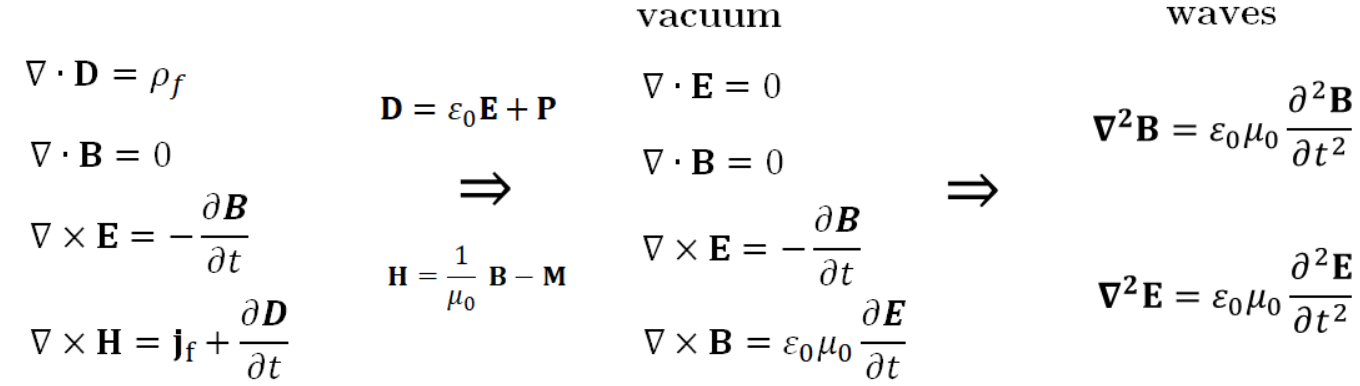
\includegraphics[width=1.0\linewidth]{summary.png}
    \caption*{}
\end{figure}

É fácil mostrar que as soluções para um meio sem fontes $(\rho=J=0)$, isotrópico e linear (em que $\mu$ e $\varepsilon$ não dependem de $E$ e $H$) são:

\begin{equation}
    \grad^2{\textbf{H}}=\varepsilon\mu\frac{\partial^2\textbf{H}}{\partial t^2}\;\;\;\;\;\;\;\;\;\;\;\;\;\grad^2{\textbf{E}}=\varepsilon\mu\frac{\partial^2\textbf{E}}{\partial t^2}
\end{equation}

\subsection{Encontrando o campo \textbf{H} a partir de \textbf{E}}\label{encontrando.campo.h}

Dado:

\begin{equation}
    E(\textbf{r},t)=E_0e^{i(\textbf{k}\vdot\textbf{r}+\omega t)}
\end{equation}

Podemos usar a Equação \ref{curlEvac}:
\begin{equation}
    \curl{\textbf{E}}=-\frac{\partial\textbf{B}}{\partial t}
\end{equation}

Para escrever:
\begin{equation}
    E_0\curl{e^{i(\textbf{k}\vdot\textbf{r}+\omega t)}}=-\frac{\partial\textbf{B}}{\partial t}
\end{equation}

Se, por exemplo, a onda plana se propaga na direção $\hat{\textbf{z}}$ e é polarizada ao longo de $\hat{\textbf{x}}$:
\begin{equation}
    \textbf{E}(\textbf{r},t)=\hat{\textbf{x}}E_0e^{-i(kz-\omega t)}
\end{equation}

Então o rotacional dá:

\begin{equation}
    \hat{\textbf{y}}\frac{\partial}{\partial z}E_0e^{-i(kz-\omega t)}=-\frac{\partial\textbf{B}}{\partial t}
\end{equation}

Resolvendo a derivada:

\begin{equation}
    -\hat{\textbf{y}}ikE_0e^{-i(kz-\omega t)}=-\frac{\partial\textbf{B}}{\partial t}
\end{equation}

E integrando no tempo:

\begin{equation}
    \textbf{B}=\hat{\textbf{y}}\frac{ik}{i\omega}E_0e^{-i(kz-\omega t)}
\end{equation}

\begin{equation}
    \textbf{B}=\hat{\textbf{y}}\frac{k}{\omega}E_0e^{-i(kz-\omega t)}
\end{equation}

Para escrever a amplitude do campo magnético, podemos usar $\textbf{H}=\frac{\textbf{B}}{\mu}$, considerando magnetização nula:

\begin{equation}
    \textbf{H}=\hat{\textbf{y}}\frac{k}{\omega\mu}E_0e^{-i(kz-\omega t)}
\end{equation}

Substituindo com o módulo de $k$:

\begin{equation}
    \textbf{H}=\hat{\textbf{y}}\frac{\omega\sqrt{\mu\varepsilon}}{\omega\mu}E_0e^{-i(kz-\omega t)}
\end{equation}

Podemos escrever como:

\begin{equation}
    \textbf{H}=\hat{\textbf{y}}\frac{1}{\eta}E_0e^{-i(kz-\omega t)}
\end{equation}

\begin{equation}
    \textbf{H}(z,t)=\hat{\textbf{y}}\frac{1}{\eta}\textbf{E}(z,t)
\end{equation}

E definir a \textbf{impedância característica} do meio:

\begin{equation}
    \eta=\sqrt{\frac{\mu}{\varepsilon}}
\end{equation}

No vácuo, $\eta_0=377\Omega$.

\subsection{O Vetor de Poynting}

O vetor de Poynting representa o fluxo direcional de energia (a transferência de energia por unidade de área por unidade de tempo $W/m^2$) de um campo eletromagnético. É definido como:

\begin{equation}
    \textbf{S}=\textbf{E}\times\textbf{H}
\end{equation}

A intensidade média no tempo é dada por:

\begin{equation}
    \langle S \rangle = \frac{1}{2}\Re(\textbf{E}\times\textbf{H}^*)
\end{equation}

A definição do vetor de Poynting se torna mais significativa quando olhamos para sua aplicação no teorema de Poynting:

\begin{equation}
    -\frac{\partial u}{\partial t}=\div{\textbf{S}}+\textbf{J}\vdot\textbf{E}
\end{equation}

Que pode ser lida da seguinte forma:

\begin{displayquote}
    A \textbf{taxa de transferência de energia} (por unidade de volume) em uma região do espaço é igual à \textbf{taxa de trabalho realizado sobre uma distribuição de carga} somada ao \textbf{fluxo de energia saindo daquela região}.
\end{displayquote}

De forma equivalente, e em melhor acordo com a escolha de sinais na representação, poderíamos dizer que:

\begin{displayquote}
    A redução na \textbf{energia eletromagnética por unidade de tempo} em um dado volume (representado pela derivada temporal da densidade de energia $u$) é igual ao \textbf{trabalho feito pelo campo elétrico \textbf{$E$}} em uma distribuição de carga (\textbf{$J$}) somado ao \textbf{fluxo resultante de energia por unidade de tempo para fora do volume}. (divergência de \textbf{$S$}).
\end{displayquote}

A representação integral deixa tudo ainda mais intuitivo.

\begin{equation}
    -\frac{\partial}{\partial t}\int_V u \,dV= \oiint_{\partial V} \textbf{S}\vdot\,dA+\int_V \textbf{J}\vdot\textbf{E}\,dV
\end{equation}

Além disso, uma análise dimensional sugere, corretamente, que o vetor de Poynting dá a pressão de radiação de uma onda eletromagnética:

\begin{equation}
    P_{rad}=\frac{\langle S \rangle}{c}
\end{equation}

\subsection{Velocidade de fase}

Se um ponto está em um pico de uma onda, com qual velocidade ele precisa se mover para continuar lá?

Se a onda é dada por:
\begin{equation*}
    e^{-i(kz-\omega t)}=\text{cte}
\end{equation*}
\begin{equation*}
    -i(kz-\omega t)=\text{cte}
\end{equation*}
\begin{equation*}
    z=\frac{\omega t}{k}+\text{cte}
\end{equation*}
\begin{equation*}
    \frac{dz}{dt}=\frac{\omega}{k}
\end{equation*}
\begin{equation*}
    \frac{dz}{dt}=v_p=\frac{1}{\sqrt{\varepsilon\mu}}
\end{equation*}
Definindo a velocidade de fase $v_p$:
\begin{equation*}
    v_p=\frac{1}{\sqrt{\varepsilon\mu}}
\end{equation*}
E o índice de refração:
\begin{equation}
    n\equiv\frac{c}{v_p}=\frac{\sqrt{\mu\varepsilon}}{\sqrt{\mu_0\varepsilon_0}}
\end{equation}
Com o índice de refração em mãos, podemos definir o vetor de onda $k$ em um meio em termos do vetor de onda no vácuo $k_0$ e $n$:
\begin{equation}
    k=k_0n
\end{equation}

Então, dentro de um dielétrico:
\begin{itemize}
    \item O comprimento de onda é reduzido por $1/n$;
    \item $k$ aumenta para $k_0n$;
    \item A velocidade de fase é reduzida para $c/n$;
    \item A frequência angular $\omega$ é mantida;
\end{itemize}

\subsection{Velocidade de grupo}

Vamos considerar as partes reais de duas ondas planas:

\begin{equation*}
    E_1(x,t)=E_0\cos((\omega+\Delta\omega)t-(k+\Delta k)x)
\end{equation*}
\begin{equation*}
    E_2(x,t)=E_0\cos((\omega-\Delta\omega)t-(k-\Delta k)x)
\end{equation*}

A Figura \ref{group.velocity} mostra as duas equações, e sua soma, no domínio da posição, usando $k=\omega=30$ e $\Delta\omega=\Delta k =1$. Isso corresponde a duas ondas com frequências e números de onda muito próximos.

\begin{figure}[H]
    \centering
    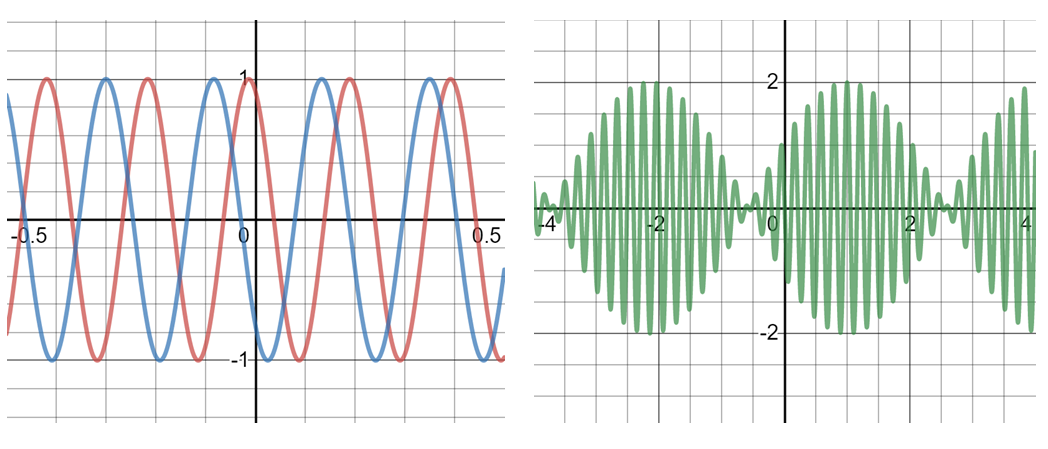
\includegraphics[width=1\linewidth]{wave packet.png}
    \caption{(a) Duas ondas planas separadas por $\Delta\omega$ e $\Delta k$ em frequência e número de onda. (b) a soma das duas ondas. Note a diferenças nas escalas dos eixos.}
    \label{group.velocity}
\end{figure}

Matematicamente, podemos escrever:
\begin{multline*}
    E_1(x,t)+E_2(x,t)=E_0\cos((\omega+\Delta\omega)t-(k+\Delta k)x)\\
    +E_0\cos((\omega-\Delta\omega)t-(k-\Delta k)x)
\end{multline*}
\begin{multline*}
    E_1(x,t)+E_2(x,t)=E_0\cos((\omega t-kx)+(\Delta\omega t-\Delta k x))\\
    +E_0\cos((\omega t - kx)-(\Delta\omega t-\Delta kx))
\end{multline*}

Usando uma identidade trigonométrica:
\begin{equation*}
    \cos(x+y)+\cos(x-y)=\cos(x)\cos(y)-\sin(x)\sin(y)+\cos(x)\cos(y)+\sin(x)\sin(y)
\end{equation*}
\begin{equation*}
    \cos(x+y)+\cos(x-y)=2\cos(x)\cos(y)
\end{equation*}
Ficamos com:
\begin{equation}
    E_1(x,t)+E_2(x,t)=2E_0\cos(\omega t-kx)\cos(\Delta\omega t-\Delta k x)    
\end{equation}

O segundo fator na última equação descreve um contorno para o pacote de ondas, e é mostrado em vermelho na Figura \ref{envelope}:

\begin{figure}[H]
    \centering
    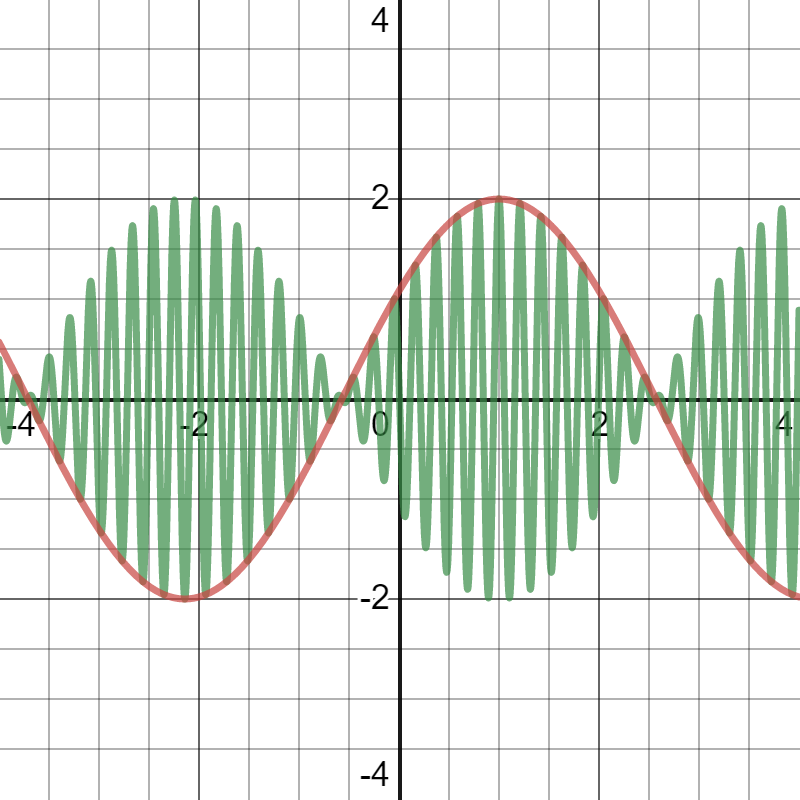
\includegraphics[width=0.5\linewidth]{envelope.png}
    \caption{O termo trigonométrico contendo as diferenças de frequência e número de onda em seu argumento descreve um contorno para o pacote de ondas, e pode ser usado para determinar a velocidade de grupo.}
    \label{envelope}
\end{figure}

Usando a mesma lógica de antes, vamos nos perguntar: quão rápido um ponto no pico da onda teria que se mover para que se mantivesse lá?
\begin{equation*}
    x(t)=\frac{\Delta\omega t}{\Delta k}+\text{constant}
\end{equation*}
A derivada temporal dá:
\begin{equation*}
    \frac{dx(t)}{dt}=v_g=\frac{\Delta\omega}{\Delta k}
\end{equation*}
E, no limite:
\begin{equation*}
    v_g=\frac{d\omega}{dk}
\end{equation*}
Por definição:
\begin{equation}
    \omega=kv_p=\frac{kc}{n}
\end{equation}
Então:
\begin{equation*}
    v_g=\frac{d}{dk}\Biggl(\frac{kc}{n}\Biggr)=\frac{c}{n}-\frac{kc}{n^2}\frac{dn}{dk}
\end{equation*}
\begin{equation*}
    \boxed{v_g=\frac{c}{n}-\lambda\frac{dn}{d\lambda}}
    \label{dispersion}
\end{equation*}

O último termo na Equação \ref{dispersion} descreve a \textbf{dispersão}. Se o índice de refração responde a uma mudança no comprimento de onda, então haverá uma mudança na velocidade de grupo associada a toda mudança no índice de refração.

\subsection{Reflexão e Refração em uma Interface Dielétrica}\label{reflexão.refraçaõ.interface}

Na Figura \ref{interface}, o vetor de onda \textbf{k} se propaga de um meio com índice de refração $n_1$ para um meio com índice $n_2$. À onda $q$ (i$\rightarrow$incidente, r$\rightarrow$refletida e t$\rightarrow$transmitida), associamos a seguinte equação para o campo elétrico:

\begin{equation}
    \textbf{E}_q(\textbf{r},t)=\hat{x}E_qe^{-i(\textbf{k}_q\vdot\textbf{r}-\omega t)}
\end{equation}

Assumindo um campo elétrico polarizado na direção $\hat{x}$:

\begin{figure}[H]
    \centering
    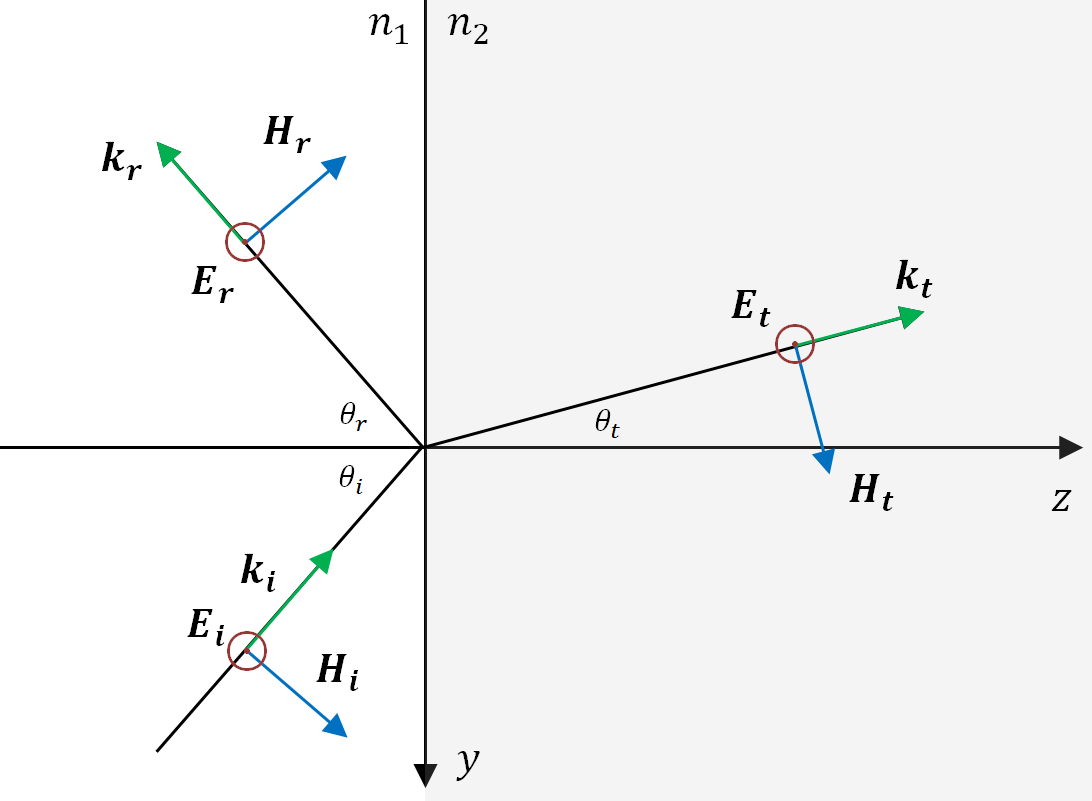
\includegraphics[width=0.8\linewidth]{bouindary.png}
    \caption{Reflexão e refração em uma interface dielétrica.}
    \label{interface}
\end{figure}

Olhando para a Figura \ref{interface}, vamos escrever o vetor de onda incidente $\textbf{k}_i$:

\begin{equation*}
    \hat{k}_i=(k_0n_1)(\hat{z}\cos\theta_i-\hat{y}\sin\theta_i)
\end{equation*}

Perceba que o módulo do vetor é dado pelo primeiro fator, que é basicamente o vetor de onda no vácuo $k_0=\omega/c$ ajustado pelo índice de refração do meio.

É só substituir isso na Equação de cima para encontrar uma descrição completa do campo elétrico incidente:

\begin{equation*}
    \textbf{E}_i(\textbf{r},t)=\hat{x}E_ie^{-i((k_0n_1)(\hat{z}\cos\theta_i-\hat{y}\sin\theta_i)\vdot\textbf{r}-\omega t)}
\end{equation*}

\begin{equation*}
    \textbf{E}_i(\textbf{r},t)=\hat{x}E_ie^{i\omega t}e^{-i(k_0n_1)(\hat{z}\cos\theta_i-\hat{y}\sin\theta_i)\vdot\textbf{r}}
\end{equation*}

Perceba que para definir totalmente o campo elétrico, foi preciso conhecer:

\begin{itemize}
    \item A direção, dada pelo vetor de onda $\hat{k}$;
    \item A polarização, dada pelo vetor unitário $\hat{x}$;
    \item A frequência, dada por $\omega$;
\end{itemize}

Os campos transmitido e refletido só diferem pelo vetor de onda, que pode facilmente ser reescrito analisando a Figura \ref{interface}:

\begin{equation*}
    \textbf{E}_r(\textbf{r},t)=\hat{x}E_re^{i\omega t}e^{-i(k_0n_1)(-\hat{z}\cos\theta_r-\hat{y}\sin\theta_r)\vdot\textbf{r}}
\end{equation*}

\begin{equation*}
    \textbf{E}_t(\textbf{r},t)=\hat{x}E_te^{i\omega t}e^{-i(k_0n_2)(\hat{z}\cos\theta_t-\hat{y}\sin\theta_t)\vdot\textbf{r}}
\end{equation*}

Para encontrar os campos magnéticos, temos que lembrar que eles precisam ser perpendiculares ao campo elétrico \textbf{e} ao vetor de onda simultaneamente. Isso define facilmente a direção de polarização.

Feito isso, vimos na seção \ref{encontrando.campo.h} que a magnitude do campo magnético é obtida dividindo a magnitude do campo elétrico pela impedância $\eta$ do meio.
Então as expressões são:

\begin{equation*}
    \textbf{H}_i(\textbf{r},t)=(\hat{z}\sin\theta_i+\hat{y}\cos\theta_i)\frac{E_i}{\eta_1}e^{i\omega t}e^{-i(k_0n_1)(\hat{z}\cos\theta_i-\hat{y}\sin\theta_i)\vdot\textbf{r}}
\end{equation*}

\begin{equation*}
    \textbf{H}_t(\textbf{r},t)=(\hat{z}\sin\theta_t+\hat{y}\cos\theta_t)\frac{E_t}{\eta_2}e^{i\omega t}e^{-i(k_0n_2)(\hat{z}\cos\theta_t-\hat{y}\sin\theta_t)\vdot\textbf{r}}
\end{equation*}

\begin{equation*}
    \textbf{H}_r(\textbf{r},t)=
    (\hat{z}\sin\theta_r-\hat{y}\cos\theta_r)
    \frac{E_r}{\eta_1}
    e^{i\omega t}
        e^{
            -i(k_0n_1)(-\hat{z}\cos\theta_r-\hat{y}\sin\theta_r)
            \vdot
            \textbf{r}
          }
\end{equation*}

Perceba que a direção foi obtida facilmente apenas trocando as funções trigonométricas que aparecem nos vetores de onda dos campos elétricos, e ajustando os sinais olhando para a Figura \ref{interface}.

\subsubsection{Condições de Contorno}

Como o campo elétrico, no caso em questão, sempre aponta na direção $\hat{x}$, e a interface está no plano $y=0$, podemos escrever a componente do campo elétrico ao longo da interface como:

\begin{equation}
    \textbf{E}_{tan}=\hat{z} \times \textbf{E}_q
\end{equation}

Lembrando que $\hat{z}\times\textbf{E}$ é uma permutação par $(y-z-x)$, e portanto o produto vetorial aponta para $+y$. Se escolhêssemos $\textbf{E}\times \hat{z}$ teríamos uma permutação ímpar $(y-x-z)$, e o produto vetorial apontaria para $-y$.

Agora vamos exigir que o \textbf{campo tangencial que chega pela esquerda da interface} seja igual ao \textbf{campo tangencial que chega pela direita da interface}:

\begin{equation}
    \hat{z}\times(\textbf{E}_i+\textbf{E}_r)\bigr|_{z=0}=\hat{z}\times\textbf{E}_t\bigr|_{z=0}
\end{equation}

Olhando para as expressões dos campos elétricos:

\begin{equation*}
    \textbf{E}_i(\textbf{r},t)=\hat{x}E_ie^{i\omega t}e^{-i(k_0n_1)(\hat{z}\cos\theta_i-\hat{y}\sin\theta_i)\vdot\textbf{r}}
\end{equation*}

\begin{equation*}
    \textbf{E}_r(\textbf{r},t)=\hat{x}E_re^{i\omega t}e^{-i(k_0n_1)(-\hat{z}\cos\theta_r-\hat{y}\sin\theta_r)\vdot\textbf{r}}
\end{equation*}

\begin{equation*}
    \textbf{E}_t(\textbf{r},t)=\hat{x}E_te^{i\omega t}e^{-i(k_0n_2)(\hat{z}\cos\theta_t-\hat{y}\sin\theta_t)\vdot\textbf{r}}
\end{equation*}

 O produto vetorial $\hat{z}\times\hat{x}$ apontará na direção $\hat{y}$ e o vetor de posição vira $\textbf{r}=(x\hat{x}+y\hat{y})$, de tal forma que apenas a componente em $\hat{y}$ sobrevive na exponencial.
 
 \begin{equation*}
    \hat{y}E_ie^{i\omega t}e^{ik_0n_1y\sin\theta_i}+
    \hat{y}E_re^{i\omega t}e^{ik_0n_1y\sin\theta_r}
    =
    \hat{y}E_te^{i\omega t}e^{ik_0n_2y\sin\theta_t}
\end{equation*}

E os termos associados à frequência podem ser cortados:

\begin{equation}
    \hat{y}E_ie^{ik_0n_1y\sin\theta_i}+
    \hat{y}E_re^{ik_0n_1y\sin\theta_r}
    =
    \hat{y}E_te^{ik_0n_2y\sin\theta_t}
    \label{continuidade.tangencial}
\end{equation}

Usando $\theta_i=\theta_r$, então podemos combinar os termos do lado esquerdo, e então tomar o valor absoluto:

 \begin{equation}
   E_i+E_r=E_t
   \label{conservacao.de.campo}
\end{equation}

Substituindo essa igualdade na Equação \ref{continuidade.tangencial}, encontramos:

\begin{equation}
    e^{ik_0n_1y\sin\theta_i}
    =
    e^{ik_0n_2y\sin\theta_t}
\end{equation}

Tirando o logaritmo e cancelando os termos comuns, chegamos na Lei de Snell:

\begin{equation}
    \boxed{n_1\sin\theta_i=n_2\sin\theta_t}
\end{equation}

Isso determina a direção da onda transmitida. O problema agora é determinar as magnitudes dos campos $E_t$, $E_r$, $H_t$ e $H_r$. Isso é resolvido aplicando as mesmas condições de continuidade para o campo magnético:

\begin{equation}
    \hat{z}\times(\textbf{H}_i+\textbf{H}_r)\bigr|_{z=0}=\hat{z}\times\textbf{H}_t\bigr|_{z=0}
\end{equation}

Assim como antes, usamos as expressões dos campos:

\begin{equation*}
    \textbf{H}_i(\textbf{r},t)=(\hat{z}\sin\theta_i+\hat{y}\cos\theta_i)\frac{E_i}{\eta_1}e^{i\omega t}e^{-i(k_0n_1)(\hat{z}\cos\theta_i-\hat{y}\sin\theta_i)\vdot\textbf{r}}
\end{equation*}

\begin{equation*}
    \textbf{H}_t(\textbf{r},t)=(\hat{z}\sin\theta_t+\hat{y}\cos\theta_t)\frac{E_t}{\eta_2}e^{i\omega t}e^{-i(k_0n_2)(\hat{z}\cos\theta_t-\hat{y}\sin\theta_t)\vdot\textbf{r}}
\end{equation*}

\begin{equation*}
    \textbf{H}_r(\textbf{r},t)=
    (\hat{z}\sin\theta_r-\hat{y}\cos\theta_r)
    \frac{E_r}{\eta_1}
    e^{i\omega t}
        e^{
            -i(k_0n_1)(-\hat{z}\cos\theta_r-\hat{y}\sin\theta_r)
            \vdot
            \textbf{r}
          }
\end{equation*}

A partir daí, tomando $z=0$, escrevendo os produtos vetoriais:

\begin{equation*}
    \hat{z}\times\textbf{H}_i(\textbf{r},t)=\Bigl(-\hat{x}\frac{E_i\cos\theta_i}{\eta_1}\Bigr)e^{i\omega t}e^{-ik_0n_1(-y\sin\theta_i)}
\end{equation*}

\begin{equation*}
    \hat{z}\times\textbf{H}_t(\textbf{r},t)=\Bigl(-\hat{x}\frac{E_t\cos\theta_t}{\eta_2}\Bigr)e^{i\omega t}e^{-ik_0n_2(-y\sin\theta_t)}
\end{equation*}

\begin{equation*}
    \hat{z}\times\textbf{H}_r(\textbf{r},t)=\Bigl(\hat{x}\frac{E_r\cos\theta_r}{\eta_1}\Bigr)e^{i\omega t}e^{-ik_0n_1(-y\sin\theta_r)}
\end{equation*}

Substituindo na condição de contorno e cortando os termos iguais:

\begin{multline*}
    \Bigl(-\frac{E_i\cos\theta_i}{\eta_1}\Bigr)e^{-ik_0n_1(-y\sin\theta_i)}+\Bigl(\frac{E_r\cos\theta_r}{\eta_1}\Bigr)e^{-ik_0n_1(-y\sin\theta_r)}=\\\Bigl(-\frac{E_t\cos\theta_t}{\eta_2}\Bigr)e^{-ik_0n_2(-y\sin\theta_t)}
\end{multline*}

Considerando $\theta_i=\theta_r$ e $n_1\sin\theta_i=n_2\sin\theta_r$:

\begin{equation*}
    \Bigl(-\frac{E_i\cos\theta_i}{\eta_1}\Bigr)+\Bigl(\frac{E_r\cos\theta_i}{\eta_1}\Bigr)=\Bigl(-\frac{E_t\cos\theta_t}{\eta_2}\Bigr)
\end{equation*}

\begin{equation*}
    \frac{(E_i-E_r)}{\eta_1}\cos\theta_i=\frac{E_t}{\eta_2}\cos\theta_t
\end{equation*}

Que pode ser reescrita usando a Equação \ref{conservacao.de.campo} ($E_t=E_i+E_r$). Usando essas equações, é fácil obter soluções para $E_r$ ou $E_t$ em relação a $E_i$:

\begin{equation*}
    \frac{E_r}{E_i}=\frac{\eta_2\cos(\theta_i)-\eta_1\cos(\theta_t)}{\eta_2\cos(\theta_i)+\eta_1\cos(\theta_t)}
\end{equation*}

Ou:

\begin{equation*}
    \frac{E_t}{E_i}=\frac{2\eta_2\cos(\theta_i)}{\eta_2\cos(\theta_i)+\eta_1\cos(\theta_t)}
\end{equation*}

É útil reescrever trocando a impedância do meio pelo índice de refração:

\begin{equation}
    \eta_i=\sqrt{\frac{\mu_0}{\varepsilon_i}}=\sqrt{\frac{\mu_0\varepsilon_0}{\varepsilon_i\varepsilon_0}}=\frac{\eta_0}{n_i}
\end{equation}

Supondo que $\mu=\mu_0$. Então:

\begin{equation}
    \frac{E_r}{E_i}=\frac{n_1\cos\theta_i-n_2\cos\theta_t}{n_1\cos\theta_i+n_2\cos\theta_t}
\end{equation}

\begin{equation}
    \frac{E_t}{E_i}=\frac{2\cos\theta_i}{(n_2/n_1)\cos\theta_1+\cos\theta_2}
\end{equation}

Essas são Equações de Fresnel para a amplitude dos campos transmitido e refletido. Podemos eliminar o grau de liberdade restante se a potência dos campos for conhecida.\pagebreak

\subsection{Reflexão Interna Total}

\begin{center}
\fbox{
    \parbox{\textwidth}{
        \centering O requisito essencial para que ocorra reflexão interna total é que a luz incidente venha pelo lado com maior índice de refração.
    }
}
\end{center}

Portanto, uma guia de onda deve consistir de um material dielétrico de alto índice de refração, cercado por um material com um índice mais baixo. A necessidade dessa diferença fica clara pela análise da Figura \ref{lei.de.snell}. No caso $n_1>n_2$ existem soluções em que $\theta_i<\pi/2$ e $\theta_t>\pi/2$ simultaneamente, o que corresponde à reflexão interna total.

\begin{figure}[H]
    \centering
    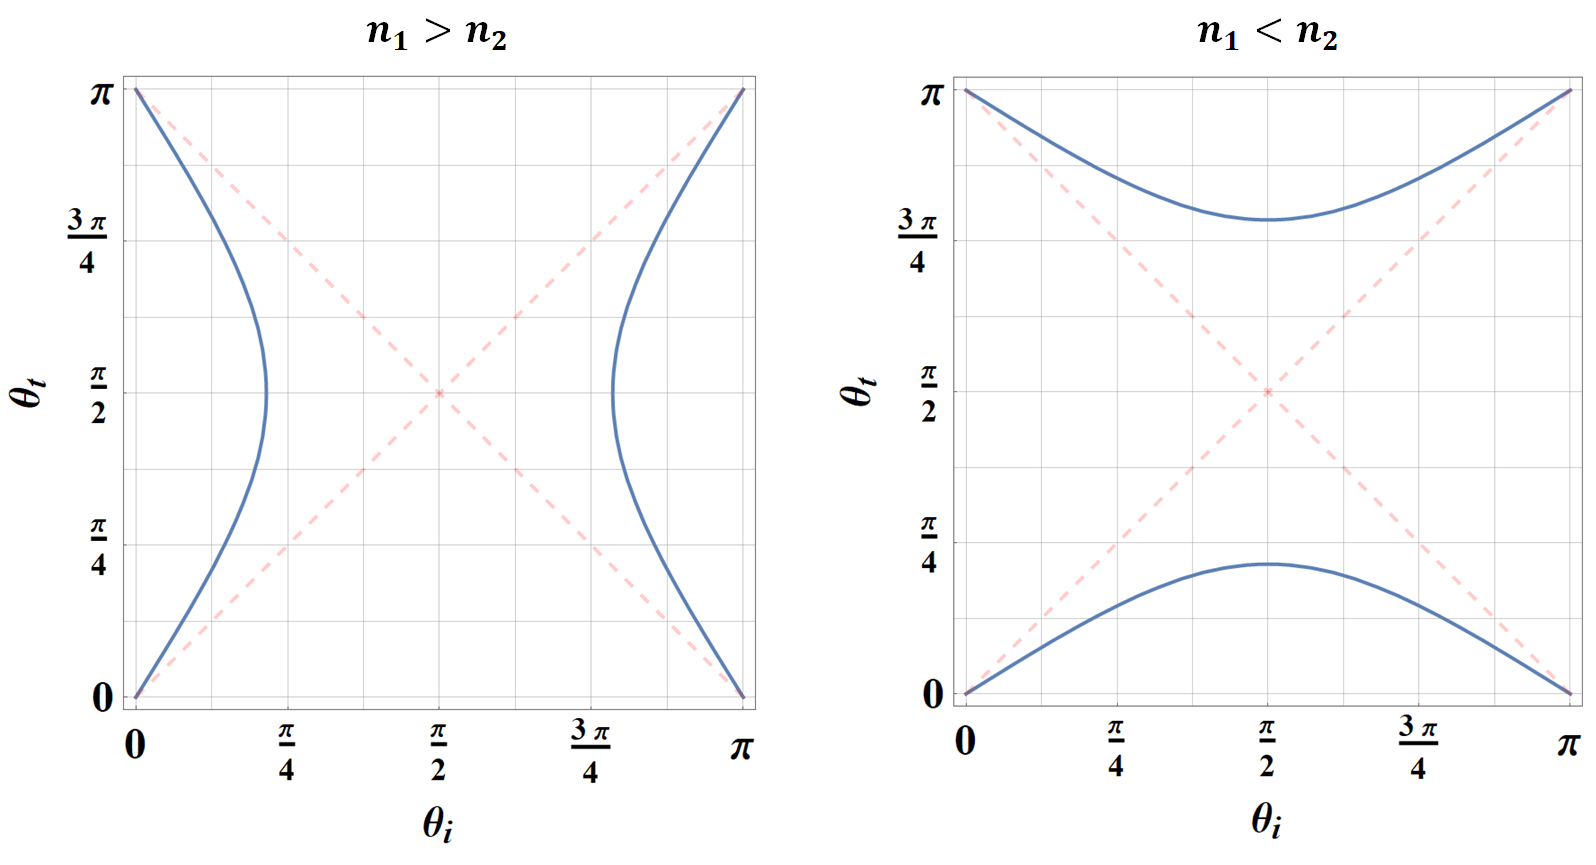
\includegraphics[width=1\linewidth]{snell solutions.png}
    \caption{Solucões da lei de Snell nos casos $n_1>n_2$ e $n_1<n_2$. A linha pontilhada indica o caso $n_1=n_2$. O caso $n_1>n_2$ permite reflexão interna total. Na prática, $\theta_t$ só assume valores no intervalo $0<\theta_t<\pi/2$.}
    \label{lei.de.snell}
\end{figure}

Como conciliar esse fenômeno com o tratamento que fizemos para a reflexão e refração por uma interface na seção anterior? Na ocasião, encontramos as seguintes expressões para os campos incidente e transmitido:

\begin{equation*}
    \begin{cases}
    \textbf{E}_i(\textbf{r},t)=\hat{x}E_ie^{i\omega t}e^{-i(k_0n_1)(\hat{z}\cos\theta_i-\hat{y}\sin\theta_i)\vdot\textbf{r}}\\
    
    \textbf{E}_t(\textbf{r},t)=\hat{x}E_te^{i\omega t}e^{-i(k_0n_2)(\hat{z}\cos\theta_t-\hat{y}\sin\theta_t)\vdot\textbf{r}}
    \end{cases}
\end{equation*}

Vamos supôr que a relação entre $E_i$ e $E_t$ seja dada em função de uma constante $E_0$ tal que:

\begin{equation}
    \begin{cases}
    E_t=\tau E_o\\
    E_i=E_0
\end{cases}
\end{equation}

Nesse caso teríamos:

\begin{equation*}
    \begin{cases}
    \textbf{E}_i(\textbf{r},t)=\hat{x}E_0e^{i\omega t}e^{-i(k_0n_1)(\hat{z}\cos\theta_i-\hat{y}\sin\theta_i)\vdot\textbf{r}}\\
    
    \textbf{E}_t(\textbf{r},t)=\tau\hat{x}E_0e^{i\omega t}e^{-i(k_0n_2)(\hat{z}\cos\theta_t-\hat{y}\sin\theta_t)\vdot\textbf{r}}
    \end{cases}
\end{equation*}

O ângulo de transmissão $\theta_t$ é determinado pela lei de Snell:

\begin{equation*}
    n_1\sin\theta_i=n_2\sin\theta_t
\end{equation*}

\begin{equation*}
    \sin\theta_t=\frac{n_1}{n_2}\sin\theta_i
\end{equation*}

\begin{equation*}
    \sqrt{1-\cos^2\theta_t}=\frac{n_1}{n_2}\sin\theta_i
\end{equation*}

\begin{equation*}
    \cos\theta_t=\sqrt{1-\frac{n_1^2}{n_2^2}\sin^2\theta_i}
\end{equation*}

Perceba que, com esse resultado, poderíamos reescrever o par de equações $\textbf{E}_i(\textbf{r},t)$, $\textbf{E}_t(\textbf{r},t)$ usando um único ângulo $\theta_i$ ao invés de $\theta_i$ e $\theta_t$.

Para evitar uma expressão longa demais, não vamos escrevê-la explicitamente. Só é importante notar que:

\begin{equation*}
    \text{Ângulo crítico}\,(\theta_i=\theta_c)\;\;\Rightarrow\;\;\frac{n_1^2}{n_2^2}\sin^2\theta_i=1\;\;\Rightarrow\;\;\cos\theta_t=0
\end{equation*}

\begin{equation*}
    \text{Ângulo acima do crítico}\,(\theta_i>\theta_c)\;\;\Rightarrow\;\;\frac{n_1^2}{n_2^2}\sin^2\theta_i>1\;\;\Rightarrow\;\;\cos\theta_t\notin \mathbb{R}
\end{equation*}

Mas veja que a expressão do campo transmitido já tem uma unidade imaginária no argumento da exponencial:

\begin{equation*}
     \textbf{E}_t(\textbf{r},t)=\tau\hat{x}E_0e^{i\omega t}e^{-i(k_0n_2)(z\cos\theta_t-y\sin\theta_t)}
\end{equation*}

Ou seja, para ângulos maiores do que o ângulo crítico, o parâmetro que media a dependência do campo com a direção $z$ (perpendicular à interface e contida no plano de incidência) se torna \textbf{real} e negativo.

Definindo o \textbf{coeficiente de atenuação} $\gamma$:

\begin{equation}
    \boxed{\gamma=k_0n_2\sqrt{1-\frac{n_1^2}{n_2^2}\sin^2\theta_i}}
\end{equation}

A expressão para o campo transmitido passa a ser:

\begin{equation*}
     \textbf{E}_t(\textbf{r},t)=\tau\hat{x}E_0e^{i\omega t}e^{-\gamma z}e^{i(k_0n_2)y\sin\theta_t}
\end{equation*}

Pela lei de Snell, é possível reescrever o argumento da última exponencial definindo a \textbf{constante de propagação} $\beta$:

\begin{equation}
    \boxed{\beta=k_0n_1\sin\theta_1}
    \label{constante.de.propagação}
\end{equation}

Então:

\begin{equation*}
     \textbf{E}_t(\textbf{r},t)=\tau\hat{x}E_0e^{i\omega t}e^{-\gamma z}e^{i\beta y}
\end{equation*}

Resumindo, no caso em que ocorre reflexão interna total, as equações para o campo incidente e transmitido ficam:

\begin{equation*}
    \begin{cases}
    \textbf{E}_i(\textbf{r},t)=\hat{x}E_0e^{-i(\frac{n_1}{n_2}\gamma z-\beta y)}\\
    
    \textbf{E}_t(\textbf{r},t)=\tau\hat{x}E_0e^{-\gamma z}e^{i\beta y}
    \end{cases}
\end{equation*}

Onde tratamos $e^{i\omega t}$ como uma fase global. Perceba que se essas equações descrevessem a luz se propagando em uma guia de onda infinita na direção $\hat{x}$, sofrendo reflexões totais sucessivas, $y$ seria a direção em que desejamos guiar a luz e $z$ seria a direção perpendicular às interfaces.

Nesse caso:
\begin{itemize}
    \item A \textbf{constante de propagação }$\beta$ mede a fase que a onda adquire enquanto se propaga ao longo da guia.
    \item O \textbf{coeficiente de atenuação} $\gamma$ mede, apropriadamente, a atenuação que a onda transmitida sofre ao penetrar no revestimento da guia.
\end{itemize}

Uma constante de propagação muito alta indica que a fase de onda sendo conduzida na guia oscila muito violentamente ao longo do comprimento.

Um coeficiente de atenuação muito alto indica que o campo está muito concentrado no 'core' da guia de onda, pois não consegue penetrar facilmente o revestimento.

\subsection{Mudança de Fase na Reflexão Total}

Vimos que, para um onda plana com polarização TE sendo refletida em uma interface dielétrica, a razão entre as intensidades $E_i$ e $E_r$ respeita a seguinte condição:

\begin{equation*}
    \frac{E_r}{E_i}=\frac{n_1\cos\theta_i-n_2\cos\theta_t}{n_1\cos\theta_i+n_2\cos\theta_t}
\end{equation*}

Lembrando que isso foi obtido na Seção \ref{reflexão.refraçaõ.interface} usando condições de continuidade para o campo elétrico nos dois lados da interface.

Vimos que na reflexão interna total ($\theta_i>\theta_{cr})$, o termo $\cos\theta_t=\sqrt{1-\frac{n_1^2}{n_2^2}\sin^2\theta_i}$ se torna imaginário. E então é conveniente escrever:

\begin{equation*}
   \frac{E_r}{E_i}=\frac{n_1\cos\theta_i-n_2\cos\theta_t}{n_1\cos\theta_i+n_2\cos\theta_t}=\abs{r}e^{i2\phi}
\end{equation*}

\begin{equation*}
    \boxed{\frac{E_r}{E_i}=\abs{r}e^{i2\phi}}
\end{equation*}

Onde $\phi$ dá a mudança de fase na reflexão interna total e $r$ dá a relação entre as magnitudes do campo incidente e transmitido.

\begin{figure}[H]
    \centering
    \includegraphics[width=0.8\linewidth]{mudança de fase na RIT.png}
    \caption{Mudança de fase para uma onda plana com polarização TE em função do ângulo de incidência para diversas razões entre os índices de refração. Perceba que a mudança de fase é nula no ângulo crítico}
    \label{fase.na.rit}
\end{figure}

\todo[inline]{ainda não entendi porque o autor divide a fase por dois para representar no gráfico.}

Isso conclui a seção sobre Equações de Maxwell.\pagebreak

\section{A Guia de Onda Plana}

Obs.: aqui, e em toda a apostila, todos os gráficos e imagens são originais.

\subsection{Infinite Slab Waveguide}

Nesse capítulo faremos um tratamento analítico da estrutura mais simples possível para uma guia de onda. Por falta de uma tradução melhor, vou me referir a essa estrutura como guia de onda "slab".

Trata-se de uma camada de dielétrico com alto índice de refração, infinito no plano $yz$ e finito na direção $x$:

\begin{figure}[H]
    \centering
    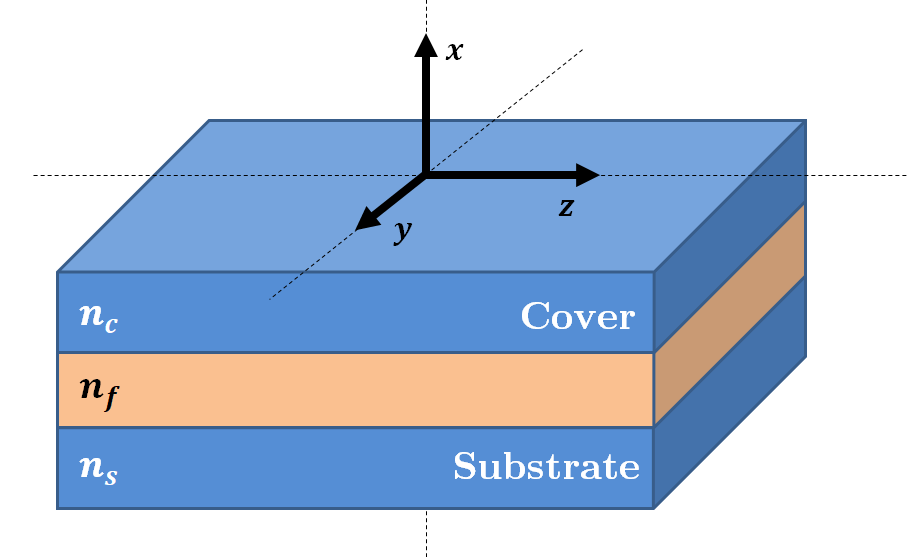
\includegraphics[width=1\linewidth]{Infinite Slab Waveguide.png}
    \caption{Uma guia de onda "slab" infinita. Apesar das cores, $n_c$ e $n_s$ não são necessariamente iguais. Por convenção, $z$ dá a direção de propagação. É comum deslocar a origem do sistema de coordenadas até uma das interfaces.}
    \label{slab.waveguide}
\end{figure}

O objetivo central dessa seção é mostrar como resolver as equações de onda com as condições de contorno das guias de onda leva naturalmente ao conceito de \textit{modos}, e então vamos explorar suas propriedades.

\subsection{Análise Eletromagnética de Guias de Onda planas}

Em primeiro lugar, vamos deslocar a origem do sistema de coordenadas da Figura \ref{slab.waveguide} para a interface entre $n_f$ e $n_C$. Na mesma Figura, uma polarização TE indica que o campo elétrico aponta na direção $y$ ($+\hat{y}$ se \textbf{k} aponta para $+\hat{z}$, e vice-versa). A polarização TM diz o mesmo para o campo $\textbf{H}$.

Vamos à solução da Equação de onda no caso TE, $\textbf{E}=E_y\hat{\textbf{y}}$:

\begin{equation*}
    \grad^2{\textbf{E}}-\varepsilon\mu\frac{\partial^2\textbf{E}}{\partial t^2}=0
\end{equation*}

Já que a dependência temporal do campo é mediada por $e^{i\omega}$:

\begin{equation*}
    \frac{\partial}{\partial t} \rightarrow i\omega\;\;\;\;\;\Rightarrow\;\;\;\;\;\frac{\partial^2}{\partial t^2} \rightarrow -\omega^2
\end{equation*}

Podemos reescrever, supondo que a guia é excitada por uma frequência $\omega_0$:

\begin{equation*}
    \grad^2E_y+\omega_0^2\mu\varepsilon E_y=0
\end{equation*}

Note a mudança do sinal na Equação acima. Sabendo que:

\begin{equation*}
    k_0=\frac{\omega_0}{c}\;\;\; \Rightarrow\;\;\; k_0n_i=\frac{\omega_0}{c}\frac{c}{v}=\frac{\omega_0}{1/\sqrt{\mu\varepsilon}}\;\;\;\Rightarrow\;\;\; k_o^2n_i^2=\omega_0^2\mu\varepsilon
\end{equation*}

Chegamos, finalmente, em:

\begin{equation}
    \boxed{\grad^2E_y+k_0^2n_i^2 E_y=0}
\end{equation}

Agora vamos usar alguns argumentos de simetria. Como a guia de onda é infinta em $yz$, a amplitude do campo só deve variar ao longo de $x$, e a fase deve variar ao longo da direção de propagação.

\begin{equation}
    \frac{\partial^2 E_y}{\partial x^2}-\beta^2E_y+k_0^2n_i^2 E_y=0
\end{equation}

\begin{equation}
    \boxed{\frac{\partial^2 E_y}{\partial x^2}+(k_0^2n_i^2-\beta^2)E_y=0}
\end{equation}

Lembrando que $\beta=k_0n_{core}\sin\theta_1$ é a constante de propagação que definimos na seção anterior, e mede o ganho de fase ao longo da direção $z$ através de $e^{i\beta z}$. O índice de $n_i$ indica que $n$ pode variar de acordo com a região em questão ($n_c, n_s, n_f$)

Agora é fácil ver que, se o termo entre parênteses for positivo, teremos uma solução oscilatória, e se for positivo teremos uma solução exponencial:

\begin{equation}
    \begin{cases}
        E_y(x)=E_0e^{\pm i\sqrt{k_0^2n_i^2-\beta^2}x}\;\;\; \beta<k_0n_i \\
        E_y(x)=E_0e^{\pm\sqrt{\beta^2-k_0^2n_i^2}x}\;\;\; \beta>k_0n_i
    \end{cases}
\end{equation}

No caso exponencial, podemos reescrever isso em termos de um coeficiente de atenuação $\gamma$, e no caso oscilatório, em termos de uma vetor de onda transversal $\kappa$:

\begin{equation}
    \begin{cases}
        E_y(x)=E_0e^{\pm i\kappa x}\;\;\; \beta<k_0n_i \\
        E_y(x)=E_0e^{\pm \gamma x}\;\;\; \beta>k_0n_i
    \end{cases}
\end{equation}

Pela definição, é fácil identificar a relação geométrica entre $\beta$, $k$ e $\kappa$, conforme a Figura \ref{transverse.wavevector}.

\begin{figure}[H]
    \centering
    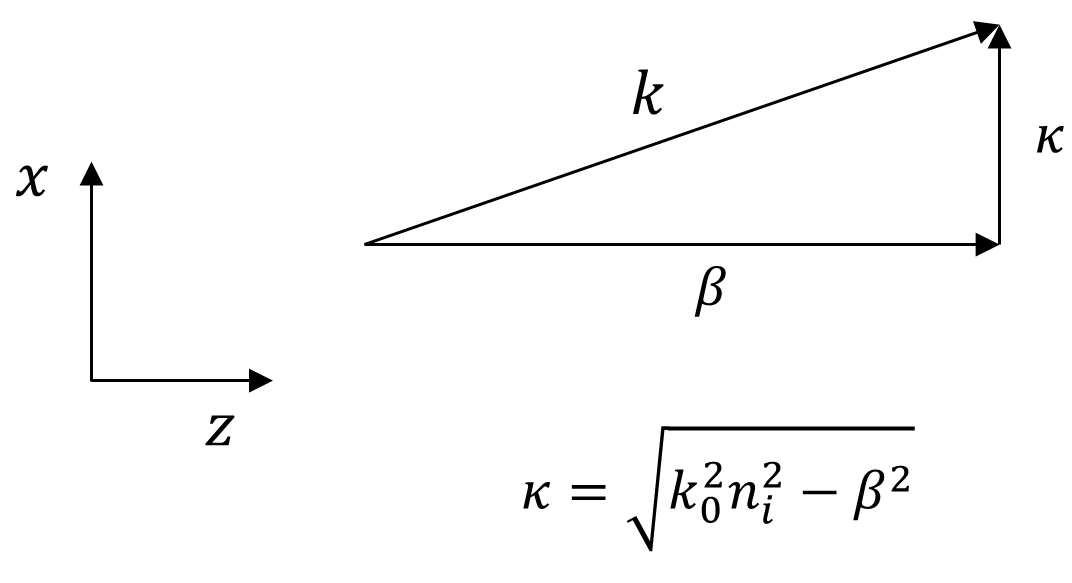
\includegraphics[width=0.4\linewidth]{transverse wavevecotr.png}
    \caption{Relação geométrica entre a constante de propagação, o vetor de onda usual e o transversal.}
    \label{transverse.wavevector}
\end{figure}

\subsection{Intuições sobre as Constantes de Propagação}

Aqui é válido fazer uma pausa para verificar se entendemos os significados de todas essas grandezas que estamos definindo.

\begin{itemize}
    \item Qual a relação entre a constante de propagação $\beta$ que definimos na seção anterior e o vetor de onda transversal que surgiu agora?
\end{itemize}

\begin{equation*}
    \beta=k_0n_1\sin\theta_1\;\;\;\;\;\;\text{em}\;\;\;\;\;\;\begin{cases}
    \textbf{E}_i(\textbf{r},t)=\hat{x}E_0e^{-i(\frac{n_1}{n_2}\gamma z-\beta y)}\\
    
    \textbf{E}_t(\textbf{r},t)=\tau\hat{x}E_0e^{-\gamma z}e^{i\beta y}
    \end{cases}
\end{equation*}

\begin{equation*}
    \kappa=\sqrt{k_0^2n_i^2-\beta^2}\;\;\;\;\;\;\text{em}\;\;\;\;\;\;E_y(x)=E_0e^{\pm i\kappa x}
\end{equation*}

Essa comparação é um pouco estranha, porque as duas constantes se referem a soluções de problemas diferentes.

A primeira vem da solução para uma onda plana sofrendo reflexão interna total em uma interface colocada ao longo de $y$. Note que $\beta$ dá o ganho de fase, em $rad/m$ ao longo da direção de propagação da onda, paralela à interface.

Esse significado é mantido na definição de $\kappa$. Na equação de onda, a derivada do campo em $z$ (implícita no laplaciano) corresponde a uma multiplicação por $\beta$. Perceba que, assim como antes, $\beta$ dá o ganho de fase ao longo da direção de propagação (antes $y$, agora $z$). \textbf{Melhor dizendo,o $\beta$ é a componente $z$ do vetor de onda.}

Perceba que o que distingue $x$ das outras direções é a finitude, e o que distingue $z$ de $y$ é a polarização TE.\\

A pergunta é: por que esse $\beta$ não é mais suficiente para descrever o ganho de fase? Por que agora ele aparece como coeficiente de $x$? A resposta está na simetria do problema. Como a guia de onda é infinita em $z$, qualquer fase que dependa \textbf{apenas} do deslocamento em $z$ é uma fase global.

Essa resposta faz mais sentido se analisarmos alguns resultados numéricos.

\pagebreak



\section{Guias de Onda Dielétricas Retangulares}

\pagebreak





%===============================================================================================================================================================================================================================================================================================================================================================================================================================================================
\chapter{Experiments in Quantum Optics}

\section{Modelos Clássicos da Luz}

A partir do tratamento que fizemos na seção \ref{Ondas.Eletromagnéticas}, sabemos que a equação de onda em um meio isotrópico e isolante é:

\begin{equation}
   \boxed{\grad^2{\textbf{E}}=\frac{1}{c^2}\frac{\partial^2\textbf{E}}{\partial t^2}}
\end{equation}

E que uma solução geral dessa equação é:

\begin{equation}
    \textbf{E}(\textbf{r},t)=E_0\textbf{p}(\textbf{r},t)\bigl[\alpha(\textbf{r},t)\exp(i\omega t)+\alpha^*(\textbf{r},t)\exp(-i\omega t)\bigr]
\end{equation}

Onde a amplitude complexa adimensional da onda pode ser escrita como:

\begin{equation}
    \alpha(\textbf{r},t)=\alpha_0(\textbf{r},t)\exp(i\phi(\textbf{r},t))
\end{equation}

Perceba que o resultado de que tratamos na Seção \ref{Ondas.Eletromagnéticas} é simplesmente um caso especial, em que:

\begin{equation*}
    \phi(\textbf{r})=-\textbf{k}\vdot\textbf{r}
\end{equation*}

Que corresponde ao caso ideal, em que uma onda monocromática plana com amplitude constante. Todas as grandezas expostas aqui, e as relações entre elas, já foram discutidas em detalhe anteriormente.

O vetor $\textbf{p}(\textbf{r},t)$ dá a polarização da onda. Tem uma direção fixa se a polarização é linear, e uma direção que oscila se a polarização. Evidentemente, sempre temos $\textbf{p}\perp\textbf{k}$.

Até aqui, nada novo.

\subsection{O Feixe Gaussiano}

Continuamos com a solução geral da equação de onda, mas pelo princípio da superposição, vamos tomar apenas um dos termos:

\begin{equation}
    \textbf{E}(\textbf{r},t)=E_0\textbf{p}(\textbf{r},t)\bigl[\alpha(\textbf{r},t)\exp(i\omega t)\bigr]
\end{equation}

Vamos supôr que o feixe se propaga na direção $z$, com polarização em $\hat{x}$. Podemos resolver a forma escalar da equação de onda. A solução é do tipo:

\begin{equation}
    E(\textbf{r},t)=\alpha(\textbf{r},t)\exp(i\omega t)
\end{equation}

Substituindo na equação de onda, e tratando a derivada temporal como uma multiplicação pela frequência angular ($i\omega$) (como já fizemos antes), chegamos na \textbf{Equação de Helmholtz}:

\begin{equation}
  \grad^2{\alpha(\textbf{r},t)}+\frac{\omega^2}{c^2}\alpha(\textbf{r},t)=0
\end{equation}

Sabendo que $k=\omega/c$, a equação de Helmholtz corresponde a:

\begin{equation}
    [\grad^2+k^2]\alpha(\textbf{r})=0
\end{equation}

\begin{equation}
    [\grad^2+k^2]\alpha_0(\textbf{r})e^{i\phi(\textbf{r},t)}=0
\end{equation}

Onde eliminamos a dependência temporal por simplicidade. É interessante já deixar claro o que queremos fazer aqui:

\begin{center}
\fbox{
    \parbox{\textwidth}{
        \centering Algumas considerações conduzem conduzem à aproximação paraxial da equação de Helmholtz (PHE). A solução da PHE é uma onda paraboloidal. Essa onda descreve um feixe gaussiano.
    }
}
\end{center}

Separando o laplaciano em uma componente transversal e uma componente longitudinal (ao longo do sentido de propagação do feixe).

\begin{equation}
    [\grad_\perp^2+\partial^2_z+k^2]\alpha_0(\textbf{r})e^{i\phi(\textbf{r},t)}=0
\end{equation}

Tomando $\textbf{k}\parallel\hat{z}$:

\begin{equation}
    [\grad_\perp^2+\partial^2_z+k^2]\alpha_0(\textbf{r})e^{-ikz}=0
\end{equation}

Quando aplicarmos a regra do produto para resolver $\partial^2_z$, só precisamos fazer $\partial^2_z\alpha_0(\textbf{r},t)\ll k\alpha_0(\textbf{r},t)$ para obter:

\begin{equation}
    \Bigl[\grad_\perp^2-2ik\frac{\partial}{\partial z}\Bigr]\alpha_0(\textbf{r})=0
\end{equation}

Essa é a \textbf{aproximação paraxial da equação de Helmholtz}, e a onda paraboloidal é uma de suas soluções:

\begin{equation}
    \alpha_0(\textbf{r},t)=\frac{\alpha_0}{q(z)}\exp\Bigr(\frac{-ik(x^2+y^2)}{2q(z)}\Bigr)\;\;\;\;\;\;\;\;\;\;\;q(z)=z+iz_o
    \label{complex.amplitude}
\end{equation}

E a solução completa é:

\begin{equation}
    \textbf{E}(\textbf{r},t)=\hat{\textbf{x}}E_0\frac{\alpha_0}{q(z)}\exp\Bigl\{-i\Bigr(\frac{k(x^2+y^2)}{2q(z)}+kz-\omega t\Bigr)\Bigr\}
\end{equation}

O feixe gaussiano é um bom modelo de um laser. Matematicamente, o feixe é a extensão de uma distribuição estável do campo em uma cavidade óptica. Em outras palavras, é um modo da cavidade se propagando livremente no espaço.

\subsubsection{Simulações}

Vamos mostrar como a Equação \ref{complex.amplitude} representa a distribuição da intensidade do campo no espaço. A intensidade é obtida tomando o módulo quadrado da equação. O procedimento analítico é trivial, e os resultados numéricos são mais instrutivos.

\begin{figure}[H]
    \centering
    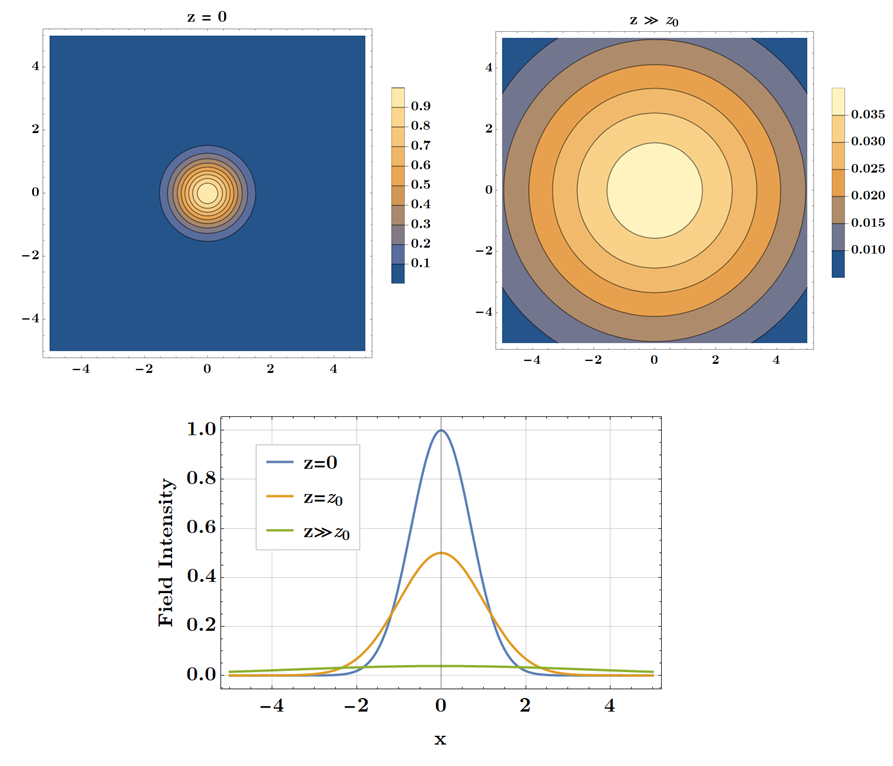
\includegraphics[width=1\linewidth]{gaussian beam.png}
    \caption{Gráficos de Intensidade do Feixe Gaussiano para diferentes posições ao longo do eixo de propagação. O feixe gaussiano preserva seu formato ao longo da direção $z$.}
    \label{slab.waveguide}
\end{figure}

\subsection{Quadrature Amplitude}\label{quatradure.amplitude}

Escrevemos a solução geral da Equação de onda da seguinte forma:

\begin{equation}
    \textbf{E}(\textbf{r},t)=E_0\textbf{p}(\textbf{r},t)\bigl[\alpha(\textbf{r},t)\exp(i\omega t)+\alpha^*(\textbf{r},t)\exp(-i\omega t)\bigr]
\end{equation}

\begin{equation}
    \alpha(\textbf{r},t)=\alpha_0(\textbf{r},t)\exp(i\phi(\textbf{r},t))
\end{equation}

Uma forma alternativa, especialmente útil para descrição em termos de fasores, é:

\begin{equation}
    \textbf{E}(\textbf{r},t)=E_0\textbf{p}(\textbf{r},t)\bigl[X_1(\textbf{r},t)\cos(\omega t)+X_2(\textbf{r},t)\sin(\omega t)\bigr]
\end{equation}

Nessa representação, as \textit{amplitudes em quadratura} $X_1$ e $X_2$ se relacionam com a amplitude complexa através de:

\begin{equation}
    \begin{cases}
        X_1(\textbf{r},t)=\alpha(\textbf{r},t)+\alpha^*(\textbf{r},t)\\
        X_2(\textbf{r},t)=i[\alpha(\textbf{r},t)-\alpha^*(\textbf{r},t)]\\
    \end{cases}
\end{equation}

Evidentemente, a fase absoluta da onda é:

\begin{equation}
    \phi_0=\arctan(\frac{X_2}{X_1})
\end{equation}

A principal motivação para introduzir essa notação, é a possibilidade de utilizá-la para representar pequenas variações na amplitude e na fase da onda. Com efeito, no limite $\alpha(t)\gg \delta X_1(t)$:

\begin{equation}
    \alpha(t)=\alpha+\delta X_1(t)+i\delta X_2(t)
\end{equation}

Onde $\delta X_1$ e $\delta X_2$ representam pequenas flutuações na amplitude e na fase, respectivamente.

\subsection{Intensidade, Energia e Potência}

Tomando a solução geral em forma escalar:

\begin{equation*}
    E(\textbf{r},t)=E_0\bigl[\alpha(\textbf{r},t)\exp(i\omega t)+\alpha^*(\textbf{r},t)\exp(-i\omega t)\bigr]
\end{equation*}

O quadrado dá:

\begin{equation*}
    E^2(\textbf{r},t)=E_0^2\;[\alpha^2(\textbf{r},r) \exp(2i\omega t)+2\alpha^*(\textbf{r},t)\alpha(\textbf{r},t)+(\alpha^*)^2(\textbf{r},t)\exp(-2i\omega t)]
\end{equation*}

Queremos calcular a energia que passa por um pequeno elemento de área $dx$, $dy$ ao longo de um intervalo $dt$. Isso é a média da quantidade acima ao longo de um grande número de ciclos óticos, e portanto depende apenas dos termos independentes da fase.

\begin{equation}
    \varepsilon(x,y,t)=2E_0^2\;\alpha(\textbf{r},t)\; \alpha^*(\textbf{r},t)\; dx dy dt
\end{equation}

A intensidade do feixe é:

\begin{equation}
    I(x,y)=\int_{1s}{2E_0^2\;|\alpha(\textbf{r},t)|^2}dt
\end{equation}

E a potência em certa área é:

\begin{equation}
    P=\iint{I(x,y)\;\;dx dy}
\end{equation}

\section{Propriedades Estatísticas da Luz Clássica}

\subsection{Origem das Flutuações}

O modelo clássico tratado até aqui assume que a luz é uma sequência contínua de ondas eletromagnéticas. Isso não é realista: Os átomos responsáveis pela emissão da luz tem um tempo de vida limitado, se esse tempo de vida é pequeno em comparação com o tempo de detecção $t_d$, o resultado de uma medição será uma intensidade média flutuante em escalas de tempo maiores que $t_d$. Além disso, os diversos átomos em uma fonte de luz a emitem de forma independente, e podem colidir uns com os outros.

Esses efeitos têm duas consequências centrais:

\begin{enumerate}
    \item Toda fonte de luz tem uma distribuição espectral.
    \item Toda fonte de luz terá algum ruído de intensidade.
\end{enumerate}

A seguir estudaremos os fundamentos desses fenômenos.

\subsection{Coerência \small{[Ref.: Loudon]}}

\subsubsection{Modelos de Fontes de Luz Caóticas}

Vamos considerar um modelo em que a dispersão das frequências emitidas é predominantemente causada por colisões elásticas entre os átomos.

Um átomo emitindo radiação com frequência $\omega_0$ será "interrompido" durante uma colisão, e então voltará a emitir uma onda idêntica, porém defasada em relação à original. Chamaremos isso de \textbf{phase-interrupting collision}.

Essa interrupções criam dispersão na distribuição de frequências uma vez que as ondas são particionadas em seções finitas cujas decomposições de Fourier contêm frequências diferentes de $\omega_0$.

Uma simulação pode ser muito útil para ilustrar esse fenômeno. Por conveniência, representei uma solução exata na Figura \ref{phase-fourier}, mas uma transformada finita traria o mesmo padrão.

\begin{figure}[H]
    \centering
    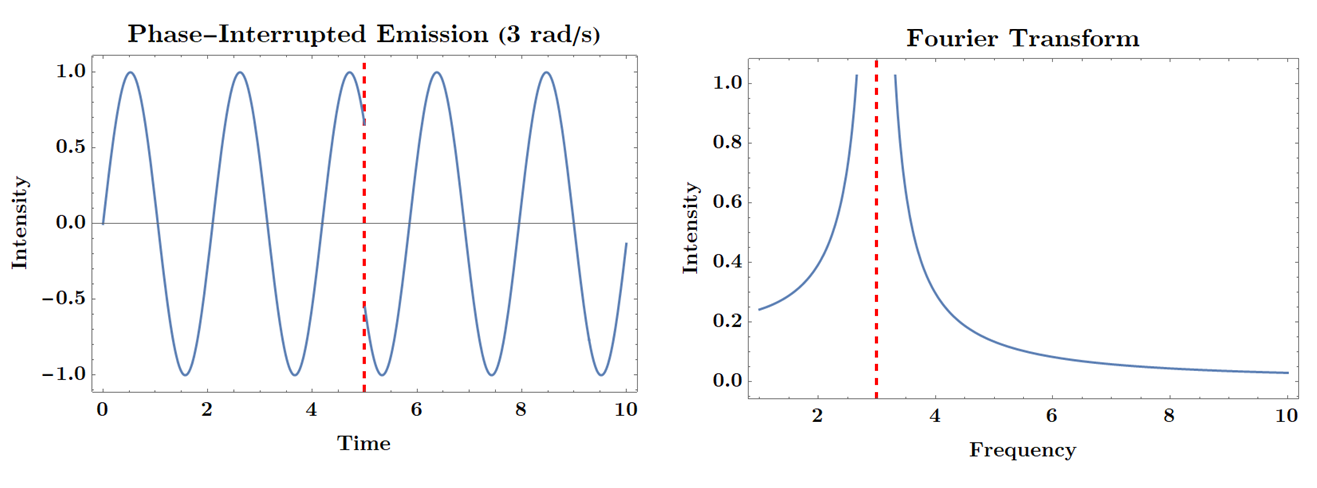
\includegraphics[width=1\linewidth]{phaseinterrupted emission.png}
    \caption{A transformada de Fourier de uma onda senoidal com frequência $\omega_0=3 rad/s$ interrompida por uma colisão instantêna em $t=5 s$ apresenta dispersão em torno de $\omega_0$. Unidades normalizadas.}
    \label{phase-fourier}
\end{figure}

Agora tome um conjunto de átomos emitindo radiação com frequência $\omega_0$, mas sobrendo interrupções de fase por colisão. Se a luz observada tem polarização fixa, podemos somar os campos algebricamente:

\begin{equation}
    E(t)=\sum^N_{i=0}{E_i(t)}
\end{equation}

\begin{equation*}
    E(t)=E_0e^{-i \omega t}\sum_{i=0}^N{e^{i\varphi_i(t)}}
\end{equation*}

Representamos o resultado dessa soma de fases (que é um processo estocástico) através de uma amplitude $a(t)$ e uma fase resultante $\varphi(t)$:

\begin{equation}
    E(t)=E_0\exp(-i \omega t)a(t)\exp(i\varphi(t))
\end{equation}

Para comparação com experimento, tomamos a média da intensidade ao longo de um ciclo de oscilação:

\begin{equation}
    \Bar{I}(t)=\frac{1}{2}\varepsilon_0c\abs{E(t)}^2=\frac{1}{2}\varepsilon_0cE_0^2a(t)^2
\end{equation}

Essa função descreve a flutuação que ocorre na intensidade de um feixe. É comum representar a intensidade no domínio do tempo com uma escala $t/\tau_c$, onde $\tau_c$ é o \textbf{tempo de coerência}, tomado como igual ao tempo médio entre colisões.

Analogamente, o \textbf{comprimento de coerência} é definido como:

\begin{equation}
    \lambda_c=c\tau_c
\end{equation}

\subsubsection{Interferômetro de Mach Zender}

As flutuações temporais das propriedades dos feixes de luz são medidos por experimentos com interferômetros. As discussões sobre o funcionamento dos beam splitters (fundamentais nesses experimentos) e do interferômetro de Mach Zender já foram feitas nas Seções \ref{beam.splitter.section} e \ref{mach.zender.section}.

Aqui vamos repetir um tratamento mais breve do interferômetro, enviesado em favor da discussão sobre coerência.

\begin{figure}[H]
    \centering
    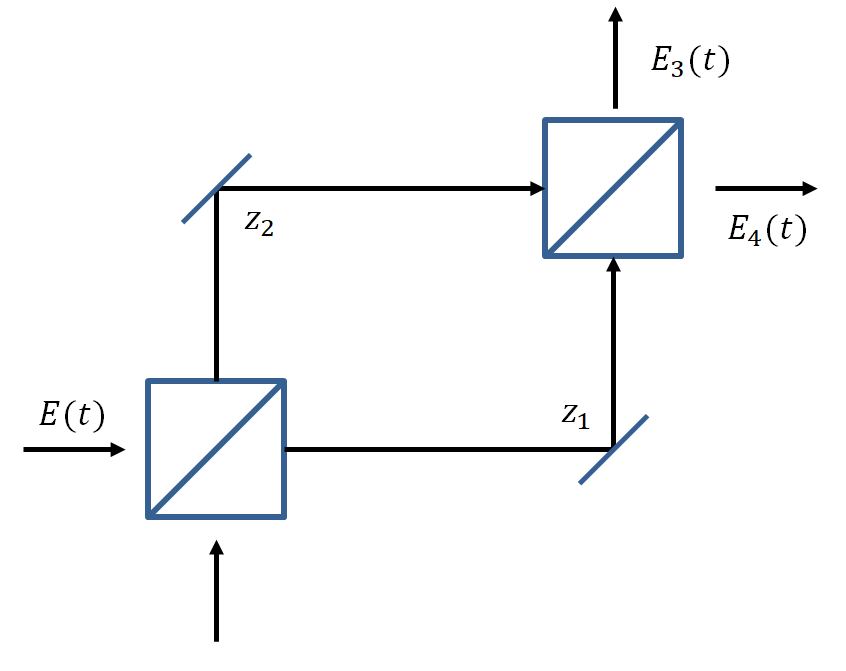
\includegraphics[width=0.5\linewidth]{mach zender loudon.png}
    \caption{Diagrama para o Interferômetro de Mach-Zender.}
    \label{mach.zender.diagram}
\end{figure}

A partir da discussão para o beam splitter, algumas considerações matemáticas devem ser evidentes a respeito da Figura \ref{mach.zender.diagram}:

\begin{equation}
    E_4(t)=\sqrt{RT}E(t_1)+\sqrt{TR}E(t_2)
\end{equation}

\begin{equation*}
    \begin{cases}
        t_1=t-(z_1/c)\\
        t_2=t-(z_2/c)
    \end{cases}
\end{equation*}

Então a intensidade da luz de saída, com a média tomada ao longo de um ciclo (usando a Equação \ref{identity.sq.abs}):

\begin{align}
    \bar{I}_4(t) & = \frac{1}{2}\varepsilon_0c\abs{E_4(t)}^2\\
                 & = \frac{1}{2}\varepsilon_0c\abs{R}\abs{T}\;\bigr[\abs{E(t_1)}^2+\abs{E(t_2)}^2+2\Re(E^*(t_1)E(t_2))\bigr]\\
\end{align}

Para um tempo muito superior a um único período, tomamos a média representada por $\langle I(t) \rangle$

\begin{equation}
    \langle I _4(t)\rangle=\frac{1}{2}\varepsilon_0c\abs{R}\abs{T}\;\bigr[\langle \abs{E(t_1)}^2\rangle+\langle \abs{E(t_2)}^2\rangle+2\Re\langle E^*(t_1)E(t_2)\rangle \bigl]
\end{equation}

\todo[inline]{Falta entender o significado geométrico do último termo}

Os dois primeiros termos representam as contribuições independentes de cada caminho para a intensidade total. As franjas de interferência surgem do último termo, que envolve A \textbf{função de correlação para os campos nos instantes $t_1$ e $t_2$}:

\begin{equation}
    \boxed{\langle E^*(t_1)E(t_2)\rangle = \frac{1}{T}\int_{T}dt_1 E^*(t_1)E(t_2)}
\end{equation}

Lembrando que $t_1$ e $t_2$ se relacionam através das diferenças de caminho conhecidas. Para um feixe de luz emitido por processos aleatórios ergódicos, e com período de medição $T$ grande o suficiente, os valores individuais de $t_1$ e $t_2$ não importam, apenas a diferença entre os dois.

Claramente, então, podemos reescrever:

\begin{equation}
    \langle E^*(t)E(t+\tau)\rangle = \frac{1}{T}\int_{T}dt E^*(t)E(t+\tau)
\end{equation}

E o \textbf{grau de coerência temporal de primeira ordem} (\textit{degree of first order coherence}) é:

\begin{equation}
    \boxed{g^{(1)}(\tau)=\frac{\langle E^*(t)E(t+\tau)\rangle}{\langle E^*(t)E(t)\rangle}}
\end{equation}

Que é apenas uma normalização da função de correlação de primeira ordem. Segue, da definição da função de correlação que:

\begin{equation}
    \langle E^*(t)E(t-\tau)\rangle = \langle E^*(t+\tau)E(t)\rangle = \langle E^*(t)E(t+\tau)\rangle^*
\end{equation}

Portanto:

\begin{equation}
    g^{(1)(-\tau)}=g^{(1)}(\tau)^*
\end{equation}

Além disso, vamos definir:

\begin{equation}
    \tau=\frac{z_1-z_2}{c}
\end{equation}

Estabelecidas essas definições, podemos reescrever a saída do interferômetro de Mach-Zender como:

\begin{equation*}
    \langle\Bar{I}_4(t)\rangle=2\abs{R}\abs{T} \Bigg( \frac{1}{2} \varepsilon_0c\langle\abs{E(t)}^2\rangle \Bigg) \Bigg{ 1+\Re(g^{(1)}(\tau)) \Bigg}
\end{equation*}

O termo entre parênteses é a intensidade média $\langle \bar{I}(t) \rangle$ do campo de entrada, então:

\begin{equation}
    \boxed{\langle\Bar{I}_4(t)\rangle=2\abs{R}\abs{T} \langle \bar{I}(t) \rangle \Big\{ 1+\Re(g^{(1)}(\tau)) \Big\}}
    \label{mach.zender.intensity.coherece}
\end{equation}

Toda a física do problema está contida na Equação \ref{mach.zender.intensity.coherece}. Vamos recapitular o que aconteceu aqui:
\begin{enumerate}
    \item No interferômetro de Mach Zender, escrevemos o campo de saída em função do campo de entrada em dois instantes diferentes, ajustados por coeficientes;
    \item A escolha desses instantes depende da diferença de caminho entre os braços do interferômetro;
    \item Na expressão para a intensidade do campo, um único termo é responsável pelos fenômenos de interferência.
    \item Esse termo depende do que definimos como \textbf{função de correlação dos campos};
    \item A forma normalizada dessa função de correlação é o \textbf{grau de coerência de primeira ordem};
    \item Ambos dependem apenas da diferença entre os dois instantes mencionados em (2). 
\end{enumerate}

\subsection{Grau de Coerência de Primeira Ordem}

Vale aplicar os resultados acima ao caso de \textit{phase-interrupted emission} (luz caótica).

Vimos que o campo resultante no caso de emissão com interrupção de fase (causada por colisões entre os átomos emissores) é:

\begin{equation*}
    E(t)=E_0e^{-i \omega_0 t}\sum_{i=0}^N{e^{i\varphi_i(t)}}
\end{equation*}


Então a função de correlação:

\begin{equation}
    \langle E^*(t)E(t+\tau) \rangle = E_0^2\exp^{-i\omega_0\tau} \times \big\langle \sum_{i=0}^N{e^{-i\varphi_i(t)}} \big\rangle \times \big\langle \sum_{i=0}^N{e^{i\varphi_i(t+\tau)}} \big\rangle
\end{equation}

Se $N$ for grande o suficiente, então todos os termos que envolvem multiplicações de fases aleatórias geradas por átomos diferentes vão gerar uma média nula.

\begin{align*}
    \langle E^*(t)E(t+\tau) \rangle & = E_0^2\exp^{-i\omega_0\tau} \times \big\langle \sum_{i=0}^N{e^{-i\varphi_i(t)}} \big\rangle \times \big\langle \sum_{i=0}^N{e^{i\varphi_i(t+\tau)}} \big\rangle\\
    & = E_0^2\exp^{-i\omega_0\tau} \times \big\langle \sum_{i=0}^N{\exp \big(i \{\varphi_i(t+\tau)-\varphi_i(t)\}\big) } \big\rangle\\
    & = N\langle E_i^*(t)E_i(t+\tau) \rangle
\end{align*}

Uma vez que todos os átomos são equivalentes. Agora, sem grandes explicações, vamos 'aceitar' um resultado da mecânica estatística. Segundo o qual a probabilidade $p(\tau)d\tau$ de que um átomo tenha um tempo de voo livre entre $\tau$ e $\tau+d\tau$ é:

\begin{equation*}
    p(\tau)d\tau=\frac{1}{\tau_0}\exp(-\frac{\tau}{\tau_0})d\tau
\end{equation*}

Como as flutuações de fase que ocorrem entre colisões produzem uma média nula, a correlação de um individual $\langle E_i^*(t)E_i(t+\tau) \rangle$ será proporcional à probabilidade de que o tempo de vôo livre seja maior do que $\tau$.\\

Então vamos retornar à equação de cima para escrever o seguinte:

\begin{align*}
    \langle E^*(t)E(t+\tau) \rangle & = E_0^2\exp^{-i\omega_0\tau} \times \big\langle \sum_{i=0}^N{e^{-i\varphi_i(t)}} \big\rangle \times \big\langle \sum_{i=0}^N{e^{i\varphi_i(t+\tau)}} \big\rangle\\
    & = E_0^2\exp^{-i\omega_0\tau} \times \big\langle \sum_{i=0}^N{\exp \big(i \{\varphi_i(t+\tau)-\varphi_i(t)\}\big) } \big\rangle\\
    & = E_0^2\exp{-i\omega\tau-(\tau/\tau_0)}
\end{align*}

De tal forma que o \textbf{grau de correlação de primeira ordem}, após normalização, será:

\begin{equation*}
    g^{(1)}(\tau)=\exp(-i\omega_0\tau-\abs{\tau}/\tau_0)
\end{equation*}

\begin{figure}[H]
    \centering
    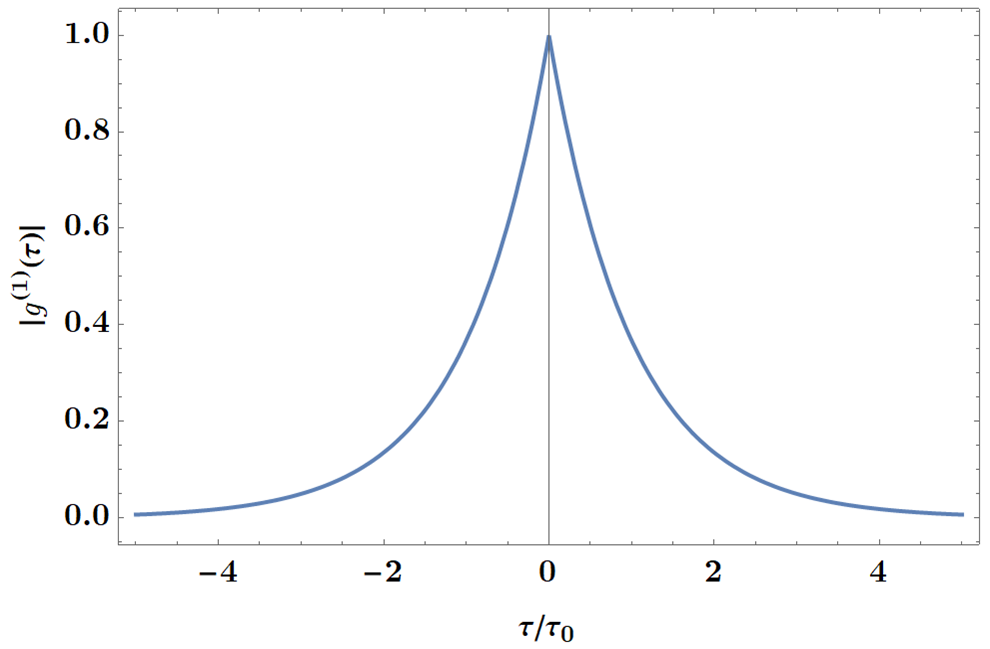
\includegraphics[width=0.75\linewidth]{degree of first order coherence phase interrupted emission.png}
    \caption{Grau de correlação de primeira ordem para \textit{phase-interrupted emission} (distribuição Lorentziana de frequências).}
    \label{degree.first.order.coherence.lorentz}
\end{figure}

A coerência de primeira ordem de ondas planas clássicas é, naturalmente, igual a $1$ para toda diferença de tempo. A chave para isso, matematicamente falando é: não há qualquer dependência temporal real na função de correlação. Na luz caótica, o tratamento mecânico-estatístico se encarrega de trazer esse termo através de distribuições de probabilidades.

\subsubsection{Franjas de Interferência e Espectro de Frequência}

Considere a transformada de Fourier finita da densidade de potência espectral do campo elétrico campo elétrico:

\begin{equation}
    f(\omega)=\frac{\abs{E_t(\omega}^2}{T}=\frac{1}{2\pi T}\int_T{dt}\int_T{dt' E^*(t)E(t')\exp{-i\omega(t-t')}}
\end{equation}

Com uma mudança de variáveis linear entre $t'$ e $\tau$:

\begin{equation}
    f(\omega)=\frac{1}{2\pi}\int_T{d\tau \langle E^*(t)E(t+\tau) \rangle \exp(i\omega\tau)}
\end{equation}

Agora basta dividir essa última equação por:

\begin{equation}
    \int_{-\infty}^{\infty}=\big\langle E^*(t)E(t) \big\rangle
\end{equation}

Que segue da definição da Delta de Dirac. Então chegamos em uma expressão para o espectro de potência do campo em função do grau de coerência de primeira ordem:

\begin{equation}
    \boxed{F(\omega)=\frac{1}{2\pi}\int_{-\infty}^{\infty} d\tau g^{(1)}(\tau)\exp(i\omega\tau)}
\end{equation}

\subsection{Grau de Coerência de Segunda Ordem}

Agora vamos considerar medidas de correlação de intensidade. A relação da coerência de primeira ordem com a intensidade era melhor descrita em termos da visibilidade $\mu$:

\begin{equation*}
    \mu=\frac{I_{máx}-I_{mín}}{I_{máx}-I_{mín}}=\abs{g^{(1)}(\tau)}
\end{equation*}

Após algumas manipulações simples. Agora vamos pensar na detecção de intensidade de dois feixes de luz que não interagiram, e tais que um deles apresenta um atrase temporal imposto antes da detecção.

As duas fotocorrentes associadas à detecção são enviadas para um medidor de correlação, que as multiplica. Nesse caso, a saída do medidor será proporcional ao \textbf{grau de coerência de segunda ordem}:

\begin{equation}
    \boxed{g^{(2)}(\tau)=\frac{\langle I(t)I(t+\tau) \rangle}{\langle I(t) \rangle^2}}
\end{equation}

Vamos discutir algumas propriedades da coerência de segunda ordem:

\begin{itemize}
    \item Pela simetria da definição, é fácil ver que a coerência de segunda ordem é par.
    \begin{equation*}
        g^{(2)}(-\tau)=g^{(2)}(\tau)
    \end{equation*}
    \item Para $\tau=0$, podemos reescrever em função da variântica de $I(t)$:
    \begin{equation*}
        g^{(2)}(0)=\frac{\langle I(t)^2 \rangle}{\langle I(t) \rangle^2}=\frac{\langle I(t)^2 \rangle-\langle I(t) \rangle^2+\langle I(t) \rangle^2}{\langle I(t) \rangle^2}=\frac{\Delta I^2}{\langle I \rangle^2}+1
    \end{equation*}
    \item Uma aplicação simples da desigualdade de Cauchy-Schwarz dá:
    \begin{equation*}
        \langle I(t_1)I(t_1+\tau) \rangle \leq \langle I(t_1)^2 \rangle \langle I(t_1+\tau)^2 \rangle
    \end{equation*}
    \begin{equation*}
        \langle I(t_1)I(t_1+\tau) \rangle^2 \leq \langle I(t_1)^2 \rangle \langle I(t_1+\tau)^2 \rangle
    \end{equation*}
    \begin{equation*}
        \langle I(t_1)^2 \rangle = \langle I(t_1+\tau)^2 \rangle \Rightarrow \langle I(t_1)I(t_1+\tau) \rangle \leq \langle I(t_1)^2 \rangle
    \end{equation*}
    \begin{equation*}
        g^{(2)}(\tau)\leq g^{(2)}(0)
    \end{equation*}
\end{itemize}

\todo[inline]{Falta explicar melhor o penúltimo passo dessa demonstração, e entender por que esse resultado é significativo. Por  enquanto ainda parece arbitrário.}

\pagebreak

\section{Fótons}
\section{Modelos Quânticos da Luz}
\section{Photodetection Techniques}


%===============================================================================================================================================================================================================================================================================================================================================================================================================================================================

\chapter{Measuring the Quantum State of Light}

\section{Quantum Theory of Light}

\subsection{Introduction}

We will begin by discussing the representation of general quantum states, and reviewing the density operator.

The first difficulty might lie in distinguishing between ``superpositions'' and ``mixed states''. A superposition describes a quantum state in terms of the eigenkets of the chosen basis in the $n-$dimensional Hilbert space. For instance:

\begin{equation}
    \ket{\alpha}=C_+\ket{+}+C_-\ket{-}
\end{equation}

Where $C_+$ and $C_-$ are complex numbers. This could describe, for instance, the state of a silver atom right after leaving an oven, and before passing through a Stern-Gerlach experiment set in the $\ket{+}/\ket{-}$ direction.

In this context, a mixed state would be a description of an ensemble of silver atoms, which have different probabilities of existing in a given $\ket{\alpha^{(i)}}$ state. The average of an observable in this ensemble is then defined as:

\begin{equation}
    [A]=\sum_{i}\omega_i\bra{\alpha^{(i)}}A\ket{\alpha^{(i)}}
\end{equation}

Where the $\omega_i$'s are the statistical weights of each possible state in the ensemble. Let us use this definition to write the \textbf{density operator}.

\begin{align}
    [A] &=\sum_{i}\omega_i\bra{\alpha^{(i)}}A\ket{\alpha^{(i)}}\\
    &=\sum_{i}\omega_i\bra{\alpha^{(i)}}A\big(\sum_{a'}\ket{a'}\bra{a'}\big)\ket{\alpha^{(i)}}\\
    &=\sum_{i}\sum_{a'}\omega_i\bra{\alpha^{(i)}}\ket{a'}\bra{a'}\ket{\alpha^{(i)}}a'\\
    &=\sum_{i}\sum_{a'}\omega_i\abs{\braket{a'}{\alpha^{(i)}}}^2a'
\end{align}

Which provides a good intuition of what this expected value is supposed to represent. The squared term in the last expression is, obviously, the probability that a $\ket{\alpha^{(i)}}$ will be measured to be in the $\ket{a'}$ eigenstate. We could, however, have taken a different term in simplifying this expression:

\begin{align}
    [A] &=\sum_{i}\omega_i\bra{\alpha^{(i)}}A\ket{\alpha^{(i)}}\\
    &=\sum_{i}\omega_i\bra{\alpha^{(i)}}A\big(\sum_{a'}\ket{a'}\bra{a'}\big)\ket{\alpha^{(i)}}\\
    &=\sum_{i}\sum_{a'}\omega_i\bra{\alpha^{(i)}}A\ket{a'}\bra{a'}\ket{\alpha^{(i)}}\\
    &=\sum_{i}\sum_{a'}\omega_i\bra{a'}\ket{\alpha^{(i)}}\bra{\alpha^{(i)}}A\ket{a'}\\
    &=\sum_{i}\sum_{a'}\bra{a'}\omega_i\ket{\alpha^{(i)}}\bra{\alpha^{(i)}}A\ket{a'}\\
    &=\sum_{a'}\bra{a'}\Big(\sum_{i}\omega_i\ket{\alpha^{(i)}}\bra{\alpha^{(i)}}\Big)A\ket{a'}\\
    &=\sum_{a'}\bra{a'}\rho A\ket{a'}\\
    &=\Tr{\rho A}
\end{align}

Where we have defined the \textbf{density operator}:

\begin{equation}
    \boxed{\rho=\sum_{i}\omega_i\ket{\alpha^{(i)}}\bra{\alpha^{(i)}}}
\end{equation}

We'll demonstrate its properties as we go.

\subsection{The electromagnetic oscillator}

Here's a complex vector function:

\begin{equation}
    \textbf{u}(x,t)=\hat{z}\;u_0\exp\big(i(kx-\omega t)\big)
\end{equation}

It represents a \textbf{spatial-temporal} mode. It is a framework in space and time that may be excited by the quantum field ``light''. The function above is a measure of the strength of such an excitation.

It would now be convenient to simply postulate that:

\begin{equation}
    \hat{E}=u^*(x,t)\hat{a}+u(x,t)\hat{a}^\dag
\end{equation}

But this is quite hard to digest. Let us try to make it somewhat more intuitive.

\subsubsection{\#1 Comment: The Quantization Cavity}

Consider a cubic region of space of side $L$. It is reasonable to expand the vector potential inside the cavity as a sum of contributions from the modes:

\begin{equation}
    \textbf{A}(\textbf{r},t)=\sum_{\textbf{k}}\sum_{\lambda}\textbf{e}_{\textbf{k}\lambda} A_{\textbf{k}\lambda}(\textbf{r},t)
\end{equation}

Solving the wave equation inside the cavity will give a familiar result for the vector potential modes:

\begin{equation}
    A_{\textbf{k},\lambda}(\textbf{r},t)=A_{\textbf{k}\lambda}\exp(-i\omega_kt+i\textbf{k}\vdot\textbf{r})+A^{*}_{\textbf{k}\lambda}\exp(i\omega_kt-i\textbf{k}\vdot\textbf{r})
\end{equation}

Finally, it is possible to show that the radiative energy of a single mode is given by:

\begin{equation}
    E_{\textbf{k}\lambda}=\epsilon_0 V\omega_k^2(A_{\textbf{k}\lambda}A^*_{\textbf{k}\lambda}+A^*_{\textbf{k}\lambda}A_{\textbf{k}\lambda})
\end{equation}

We haven't demonstrated all of these results, but they all align pretty well with out intuition. The next step in our demonstration is to discuss the quantum harmonic oscillator, and notice that \textbf{its} energy is described by a very similar expression.

\subsubsection{\#2 Comment: Quantum Mechanical Oscillator}

The Hamiltonian for a quantum mechanical oscillator in one dimension is:

\begin{equation}
    \hat{H}=\frac{\hat{p}^2}{2m}+\frac{1}{2}m\omega^2\hat{q}^2
\end{equation}

Where the position and momentum operators obey the usual commutation relation:

\begin{equation}
    \comm{\hat{q}}{\hat{p}}=i\hbar
\end{equation}

It is well known that the annihilation and creation operators may be written as follows:

\begin{equation}
    \hat{a}=\frac{1}{\sqrt{2m\hbar\omega}}(m\omega \hat{q} + i\hat{p})
\end{equation}

\begin{equation}
    \hat{a}^{\dag}=\frac{1}{\sqrt{2m\hbar\omega}}(m\omega \hat{q}-i\hat{p})
\end{equation}

Or, conversely:

\begin{equation}
    \hat{q}=\sqrt{\frac{\hbar}{2m\omega}}(\hat{a}^{\dag}+\hat{a})
\end{equation}

\begin{equation}
    \hat{p}=i\sqrt{\frac{m\hbar\omega}{2}}(\hat{a}^{\dag}-\hat{a})
\end{equation}

Now, when we multiply the two:

\begin{align}
    \hat{a}\hat{a}^{\dag}&=\frac{1}{2m\omega\hbar}(\hat{p}^2+m^2\omega^2\hat{q}^2-im\omega \hat{q}\hat{p}+im\omega \hat{p}\hat{q})\\
            &=\frac{1}{\hbar\omega}(\hat{H}+\frac{1}{2}\hbar\omega)
\end{align}
\begin{align}
    \hat{a}^{\dag}\hat{a}&=\frac{1}{2m\omega\hbar}(\hat{p}^2+m^2\omega^2\hat{q}^2+im\omega \hat{q}\hat{p}-im\omega \hat{p}\hat{q})\\
            &=\frac{1}{\hbar\omega}(\hat{H}-\frac{1}{2}\hbar\omega)
\end{align}

An obvious way to rewrite the Hamiltonian comes up:

\begin{equation}
    \hat{H}=\frac{1}{2}\hbar\omega(\hat{a}\hat{a}^{\dag}+\hat{a}^{\dag}\hat{a})=\hbar\omega\Big(\hat{a}^{\dag}\hat{a}+\frac{1}{2}\Big)
\end{equation}

Now let us use this expression to define the \textbf{quadrature operators}. At first, we may simply use them as a way to work with dimensionless forms of position and momentum operators. 

\begin{equation}
    \hat{X}=\sqrt{\frac{m\omega}{2\hbar}}\hat{q}=\frac{1}{2}(\hat{a}^{\dag}+\hat{a})
\end{equation}

\begin{equation}
    \hat{Y}=\sqrt{\frac{1}{2m\hbar\omega}}\hat{p}=\frac{1}{2}i(\hat{a}^{\dag}-\hat{a})
\end{equation}

Which will lead us to the following expression for the Hamiltonian:

\begin{equation}
    \hat{H}=\hbar\omega(\hat{X}^2+\hat{Y}^2)
\end{equation}

And the inverse relations:

\begin{equation}
    \hat{a}=\hat{X}+i\hat{Y}
\end{equation}

\begin{equation}
    \hat{a}^{\dag}=\hat{X}-i\hat{Y}
\end{equation}

Using the known uncertainty relations for position and momentum, we can write the following \textbf{quadrature uncertainty relations}:

\begin{equation}
    (\Delta \hat{X})^2(\Delta \hat{Y})^2 \ge \frac{1}{16}
\end{equation}

\subsubsection{\#3 Comment: Quantization of the electromagnetic field}

The electromagnetic field is quantized by the association of a quantum mechanical oscillator mode with each mode $\textbf{k}\lambda$ of the radiation field in the quantization cavity. We are now in a much better position to digest the previous leap. Comparing the energy radiated by one electromagnetic field mode in the quantization cavity:

\begin{equation}
    E_{\textbf{k}\lambda}=\epsilon_0 V\omega_k^2(A_{\textbf{k}\lambda}A^*_{\textbf{k}\lambda}+A^*_{\textbf{k}\lambda}A_{\textbf{k}\lambda})
\end{equation}

To the energy in a quantum mechanic oscillator defined by the same frequency as the mode:

\begin{equation}
    H_{\textbf{k}\lambda}=\frac{1}{2}\hbar\omega(\hat{a}_{\textbf{k}\lambda}\hat{a}_{\textbf{k}\lambda}^{\dag}+\hat{a}_{\textbf{k}\lambda}^{\dag}\hat{a}_{\textbf{k}\lambda})
\end{equation}

We reach the following analogy:

\begin{equation}
    \begin{cases}
        A_{\textbf{k}\lambda}\rightarrow\sqrt{\frac{\hbar}{2\epsilon_0V\omega_k}}\hat{a}_{\textbf{k}\lambda}\\[0.5cm]
        A^*_{\textbf{k}\lambda}\rightarrow\sqrt{\frac{\hbar}{2\epsilon_0V\omega_k}}\hat{a}^{\dag}_{\textbf{k}\lambda}
    \end{cases}
\end{equation}

And the vector potential will become:

\begin{equation}
    \textbf{A}(\textbf{r},t)=\sum_{\textbf{k}}\sum_{\lambda}\textbf{e}_{\textbf{k}\lambda} A_{\textbf{k}\lambda}(\textbf{r},t)
\end{equation}

\begin{equation}
    A_{\textbf{k},\lambda}(\textbf{r},t)=\sqrt{\frac{\hbar}{2\epsilon_0V\omega_k}}\Big[\hat{a}_{\textbf{k}\lambda}\exp(-i\omega_kt+i\textbf{k}\vdot\textbf{r})+\hat{a}^{\dag}_{\textbf{k}\lambda}\exp(i\omega_kt-i\textbf{k}\vdot\textbf{r})\Big]
\end{equation}

There are still some formal differences with the results we were originally attempting to digest. Still, the intuition is all here. Annihilation and creation operators are not hermitian, so they cannot represent physical observables. But the electric and magnetic fields may be written in terms of such operators, much like the position and momentum operators were.

So now, let us pick up where we left off.

\subsubsection{Continuing...}

The electric field strength is given by:

\begin{equation}
    \hat{E}=u^*(x,t)\hat{a}+u(x,t)\hat{a}^\dag
\end{equation}

The photon number operator accounts for the number of photons in the chosen spatial-temporal mode:

\begin{equation}
    \hat{n}=\hat{a}^\dag \hat{a}
\end{equation}

And the phase-shifting operator provides the amplitude $a$ with a phase shift $\theta$:

\begin{equation}
    \hat{U}(\theta)=\exp(-i\theta\hat{n})
\end{equation}

In order to understand its effect on the annihilation operator, let us solve the following differential equation:

\begin{align*}
    \frac{d}{d\theta}(\hat{U^{\dag}}\hat{a}\hat{U})&=i\hat{n}\hat{U^{\dag}}\hat{a}\hat{U}-i\hat{U^{\dag}}\hat{a}\hat{U}\hat{n}\\
    &=\hat U i \comm{\hat n}{\hat a}\hat U\\
    &=\hat U^{\dag}i\comm{\hat a^{\dag}}{a^{\dag}}\hat a \hat U\\
    &=-i\hat U^{\dag}\hat a \hat U
\end{align*}

Solving it yields:

\begin{equation}
    \therefore\;\;\; \hat U(\theta) \hat a \hat U(\theta)=Ce^{-i\theta}
\end{equation}

Imposing the initial condition $\hat U(0)\hat a \hat U(0)=\hat a$:

\begin{equation}
    \boxed{\hat U(\theta) \hat a \hat U(\theta)=\hat ae^{-i\theta}}
\end{equation}

Finally, we once again introduce the quadrature operators, \textbf{only with normalized units} ($h=1$):

\begin{equation}
    \begin{cases}
        \hat q = \frac{1}{\sqrt{2}}(\hat a^{\dag}+\hat a)\\[0.3cm]
        \hat p = \frac{i}{\sqrt{2}}(\hat a^{\dag}-\hat a)\\[0.3cm]
        \comm{\hat q}{\hat p}=i\\[0.3cm]
        \hat H=\hat n +\frac{1}{2}=\frac{\hat q^2}{2}+\frac{\hat p^2}{2}
    \end{cases}
\end{equation}

\subsection{Single mode states}

What follows is a discussion of different states of the electromagnetic oscillator.

\subsubsection{Quadrature states}

Quadrature states are eigenstates of the quadrature operators:

\begin{equation}
    \hat q \ket{q}=q\ket{q}
\end{equation}
\begin{equation}
    \hat p \ket{p}=p\ket{p}
\end{equation}

Such states must have continuous spectra, obeying:

\begin{itemize}
    \item Orthogonality
    \begin{equation*}
        \braket{q}{q'}=\delta(q-q')\;\;\;\text{and}\;\;\;\braket{p}{p'}=\delta(p-p')
    \end{equation*}
    \item Completeness
    \begin{equation*}
        \int_{-\infty}^{\infty}\ket{q}\bra{q}dq\;\;\;\text{and}\;\;\;\int_{-\infty}^{\infty}\ket{p}\bra{p}dp
    \end{equation*}
    \item Connection through the Fourier transform:
    \begin{equation*}
        \ket{q}=\frac{1}{\sqrt{2\pi}}\int_{-\infty}^{\infty}\exp(-iqp)\ket{p}dp\;\;\;\text{and}\;\;\;\ket{p}=\frac{1}{\sqrt{2\pi}}\int_{-\infty}^{\infty}\exp(-iqp)\ket{q}dq
    \end{equation*}
    \item Quadrature wave functions representations. Whose absolute squared value gives the quadrature probability distributions:
    \begin{equation*}
        \psi(q)=\braket{q}{\psi}\;\;\;\text{and}\;\;\;\Tilde{\psi}(p)\braket{p}{\psi}
    \end{equation*}
\end{itemize}

\subsubsection{Fock states}

Fock states are eigenstates of the the photon-number operator:

\begin{equation}
    \hat n \ket{n}=n\ket{n}
\end{equation}

We have already discussed at some length how these states behave under the effect of the creation and annihilation operators. Let us discuss some quadrature representations of different Fock states.

Consider the following situation:

\begin{equation}
    \hat{n}\ket{0}=\hat a^{\dag}\hat a\ket{0}=0
\end{equation}

Clearly there are two solutions: (1) $\hat a\ket{0}=0$ or (2) $\hat{a}^{\dag}(\hat a\ket{0})=0$. The latter leads non-normalisable wave function, which therefore has no physical meaning. We will concentrate on the former:

\begin{equation}
    \hat a \ket{0}=0
\end{equation}

Rewriting the annihilation operator in terms of the quadratures:

\begin{equation*}
    \frac{1}{\sqrt{2}}(\hat q+i\hat p)\ket{0}=0
\end{equation*}

Multiplying by $\bra{q}$:

\begin{equation*}
    \frac{1}{\sqrt{2}}(\hat q+i\hat p)\braket{q}{0}=0
\end{equation*}
\begin{equation*}
    \frac{1}{\sqrt{2}}(\hat q+i\hat p)\psi_0(q)=0
\end{equation*}

Substituting $q=-i\frac{\partial}{\partial q}$:

\begin{equation}
        \frac{1}{\sqrt{2}}\Big(\hat q+\frac{\partial}{\partial q}\Big)\psi_0(q)=0
\end{equation}

Whose solution is given by:

\begin{equation}
    \psi_0(q)=\pi^{-1/4}\exp\Big(-\frac{q^2}{2}\Big)
\end{equation}

Therefore, even in a complete vacuum, quadratures are still fluctuating. A similar quadrature representaion could be found for all other Fock states:

\begin{equation}
    a^{\dag}\ket{n-1}=\sqrt{n}\ket{n}
\end{equation}

\begin{equation}
    a^{\dag}\psi_{n-1}(q)=\sqrt{n}\psi_n(q)
\end{equation}

\begin{equation}
    \frac{1}{\sqrt{2}}\Big(q-\frac{\partial}{\partial q}\Big)\psi_{n-1}(q)=\sqrt{n}\psi_n(q)
\end{equation}

And the general solution is:

\begin{equation}
    \psi_n(q)=\frac{H_n(q)}{\sqrt{2^nn!\sqrt{\pi}}}\exp\Big( -\frac{q^2}{2} \Big)
\end{equation}

We are now able to plot the quadrature wave functions for some Fock states, as shown in Figure \ref{quadrature.wave.functions}:

\begin{figure}[H]
    \centering
    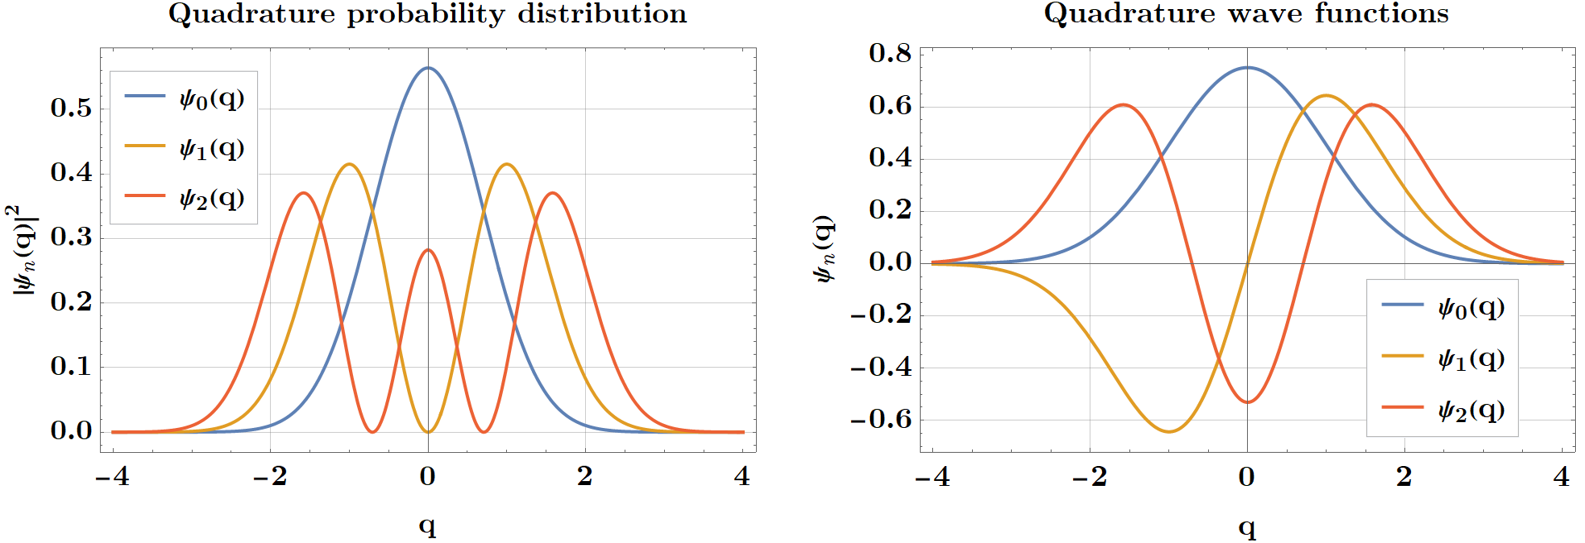
\includegraphics[width=1.0\linewidth]{quadrature wave functinos.png}
    \caption{Quadrature wave functions for Fock states.}
    \label{quadrature.wave.functions}
\end{figure}

The above considerations show that there exists a unique vacuum state for the electromagnetic oscillator, and that all Fock states can be described as excitations of the vacuum. Therefore, the Fock states must form a complete and orthonormal set:

\begin{equation}
    \sum_{n=0}^{\infty}\ket{n}\bra{n}=1
\end{equation}

\begin{equation}
    \braket{n}{n'}=\delta_{nn'}
\end{equation}

The Fock states form the most commonly used Hilbert space basis in quantum optics.

\subsection{Coherent states}

Coherent states are eigenstates of the annihilation operator:

\begin{equation}
    \hat a\ket{\alpha}=\alpha\ket{\alpha}
\end{equation}

Obs.: one immediate consequence of this definition is that vacuum states are coherent states.

Given that the annihilation operator is not hermitian, its eigenvalues are not real. Therefore we may write $\alpha=\abs{\alpha}e^{î\arg(\alpha)}$.

If we calculate the expected value for the Hamiltonian relative to the coherent state:

\begin{equation}
    \hat H = \hat a^{\dag}\hat a+\frac{1}{2}
\end{equation}
\begin{equation}
    \bra{\alpha}\hat H\ket{\alpha}=\abs{\alpha}^2+\frac{1}{2}
\end{equation}

If we look for the operator which displaces the amplitude by the complex number $\alpha$:

\begin{equation}
    \hat D^{\dag}(\alpha)\hat a\hat D(\alpha)=\hat a+\alpha
\end{equation}

The result will be:

\begin{equation}
    \hat D(\alpha)=\exp(\alpha \hat a^{\dag}-\alpha^*\hat a)
\end{equation}

What happens when we apply the annihilation operator to the displaced coherent state $\hat D(-\alpha)\ket{\alpha}$?

\begin{align}
    \hat a \big( \hat D(-\alpha)\ket{\alpha}\big)&=\hat D(-\alpha)\hat D^{\dag}(-\alpha)\hat a \big( \hat D(-\alpha)\ket{\alpha}\big)\\
    &=\hat D(-\alpha)\big(\hat D^{\dag}(-\alpha)\hat a  \hat D(-\alpha)\big)\ket{\alpha}\\
    &=\hat D(-\alpha)(\hat a -\alpha)\ket{\alpha}\\
    &=0
\end{align}

This implies that:

\begin{equation}
    \boxed{\hat D(-\alpha)\ket{\alpha}=\ket{0}}
\end{equation}

Consequently, \textbf{coherent states are displaced vacuums}. Which does not mean that coherent states are physically similar to vacuum states. They only have some quantum noise properties in common.

Now let us write the quadrature wave functions for the coherent states. If the complex amplitude $\alpha$ is given in terms of its real and imaginary parts:

\begin{equation}
    \alpha=\frac{1}{\sqrt{2}}(q_0+ip_0)
\end{equation}

The displacement operator becomes:

\begin{align*}
    \hat D(\alpha)  & =\exp(\alpha \hat a^{\dag}-\alpha^*\hat a)\\
                    & =\exp \Big( \frac{1}{\sqrt{2}}(q_0+ip_0) \hat a^{\dag}-\frac{1}{\sqrt{2}}(q_0+ip_0)^* \hat a\Big)\\
                    & =\exp\Big(\frac{1}{\sqrt{2}}(q_0+ip_0) \frac{1}{\sqrt{2}}(\hat q-i\hat p)-\frac{1}{\sqrt{2}}(q_0-ip_0) \frac{1}{\sqrt{2}}(\hat q+i\hat p)\Big)\\
                    &=\exp\Big(ip_o\hat q- iq_0\hat p\Big)
\end{align*}

Using the Baker-Hausdorff formula, we may simplify this result to write:

\begin{equation}
    \hat D(\alpha)=\exp\Big(\frac{ip_0q_0}{2}\Big)\exp(-iq_0\hat p)\exp(ip_0\hat q)
\end{equation}

Once again, if we write $\hat p = -i\partial/\partial q$:

\begin{equation}
    \hat D(\alpha)=\exp\Big(\frac{ip_0q_0}{2}\Big)\exp\Big(-q_0\frac{\partial}{\partial q}\Big)\exp(ip_0\hat q)
\end{equation}

it is clear that the second exponential becomes a translation operator, which could act on $\psi(q)$ to turn it into $\psi(q-q_0)$. Therefore, we can find a position representation for any coherent state, simply by applying $D(\alpha)$ to the position representation of the vacuum state:

\begin{align*}
    \psi_{\alpha}(q)&=\hat D(\alpha)\psi_0(q)\\
                    &= \exp\Big(\frac{ip_0q_0}{2}\Big)\exp(ip_0 q)\exp\Big(-q_0\frac{\partial}{\partial q}\Big)\psi_0(q)\\
                    &=\exp\Big(ip_0q-\frac{ip_0q_0}{2}\Big)\psi_0(q-q_0)\\
                    &=\pi^{-1/4}\exp\Big[-\frac{(q-q_0)^2}{2}+ip_0q-\frac{ip_0q_0}{2}\Big]
\end{align*}

We could go on, but this is enough: the quadrature probability distributions of coherent states are Gaussian, with the same width as the Gaussian curve for a vacuum, but shifted by the amplitudes $q_0$ and $p_0$. Notice that $\hat q$ became $q$ when we changed to the position representation. In this sense, only the vacuum fluctuations contaminate the quadrature amplitudes, ``they have just as much quadrature noise as is unavoidable''.

Now let us discuss some particle features of coherent states. We already saw in Equation \ref{operador.criador.coerente}:

\begin{equation}
   \ket{\alpha}=e^{-\frac{\abs{\alpha}^2}{2}}\sum_{n=0}^{\infty}\frac{\alpha^n}{\sqrt{n!}}\ket{n}
\end{equation}

This can be discovered simply by stating that coherent states are eigenstates of the annihilation operator, and than normalising the state. Once again, this alone is enough to demonstrate that coherent states exhibit Poissonian photon statistics.

A simple substitution yeilds an equivalent expressoin for the coherent state in the Fock basis:

\begin{equation}
   \ket{\alpha}=\exp\Bigr(-\frac{\abs{\alpha}^2}{2}\Bigl)\exp\Bigl(a^{\dag}\alpha\Bigr)\ket{0}
\end{equation}

Which describes an operator creating a coherent state form the vacuum state. This, however, is still not an unitary operator:

\begin{equation*}
    \Bigg[\exp\Bigr(-\frac{\abs{\alpha}^2}{2}\Bigl)\exp\Bigl(a^{\dag}\alpha\Bigr)\Bigg]^{\dag}=\Bigg[\exp\Bigr(-\frac{\abs{\alpha}^2}{2}\Bigl)\exp\Bigl(a\alpha^*\Bigr)\Bigg]\neq\Bigg[\exp\Bigr(-\frac{\abs{\alpha}^2}{2}\Bigl)\exp\Bigl(a^{\dag}\alpha\Bigr)\Bigg]^{-1}
\end{equation*}

We can force it to be unitary by adding a harmless term (which is equivalent to unity)

\begin{equation}
   \ket{\alpha}=\exp\Bigr(-\frac{\abs{\alpha}^2}{2}\Bigl)\exp\Bigl(a^{\dag}\alpha\Bigr)\exp\Bigl(-a\alpha^*\Bigr)\ket{0}
\end{equation}

\begin{equation}
   \ket{\alpha}=\hat D(\alpha)\ket{0}
\end{equation}


\begin{equation}
    \boxed{D(\alpha)=\exp\Bigr(-\frac{\abs{\alpha}^2}{2}\Bigl)\exp\Bigl(a^{\dag}\alpha\Bigr)\exp\Bigl(-a\alpha^*\Bigr)}
\end{equation}

\subsubsection{Uncertainty and squeezing}

Although there is a more appropriate way of demonstrating it for this particular case, let us simply state the uncertainty relation for momentum and position in normalised units:

\begin{equation}
    \Delta q \Delta p \ge \frac{1}{2}
\end{equation}

We have established that coherent states are minimum uncertainty states. However, the variances of both variables are not required to be equal. We may \textbf{squeeze} the uncertainty below the vacuum level for one of the quadratures, at the cost of enhancing uncertainty in the conjugate quadrature.

Introducing a parametrization for the deviation of the variances from their vacuum values:

\begin{equation}
    \begin{cases}
      \Delta ^2q=\frac{1}{2}e^{-2\zeta}\\
      \Delta ^2p=\frac{1}{2}e^{2\zeta}
    \end{cases}
\end{equation}

In this case, the \textbf{squeezed position wave function} is given by:

\begin{equation}
    \varphi (q) = e^{\zeta/2}\psi_0(e^{\zeta}q)
\end{equation}

And after some work, we find the following expression for the \textbf{squeezing operator}:

\begin{equation}
\hat S= \exp\Big[ \frac{\zeta}{2}(\hat a^2 - \hat a^{\dag}^2) \Big]
\end{equation}

Therefore, a squeezed vacuum state can be written as:

\begin{equation}
    \ket{\psi}=\hat S(\zeta)\ket{0}
\end{equation}

And any minimal uncertainty state can be constructed as a \textbf{displaced vacuum state}:

\begin{equation}
    \ket{\psi}=\hat  D(\alpha) \hat S(\zeta)\ket{0}
\end{equation}

The action of the squeeze operator on the quadrature is as follows:

\begin{equation}
    \hat s^{\dag}(\zeta)\hat q\hat S(\zeta)=\hat q e^{-\zeta}
\end{equation}
\begin{equation}
    \hat s^{\dag}(\zeta)\hat p\hat S(\zeta)=\hat p e^{\zeta}
\end{equation}

Writing the quadrature in terms of $\hat a$ and $\hat a^{\dag}$:

\begin{equation}
    \hat S^{\dag}(\zeta)\hat a \hat S(\zeta)=\hat a \cosh(\zeta)-\hat a^{\dag}\sinh(\eta)
\end{equation}

\todo[inline]{I'll skip a more detailed explanation of this for now. Can't understand it yet.}

\section{Quasiprobability distributions}

\section{Simple optical instruments}

\section{Homodyne detector}

Under ideal circumstances, the photon number can be measured in direct photodetection. However, another method of detection exists, in which the \textbf{field amplitudes} (the quadrature components) are measured instead.

The quadrature operators, as we have previously defined them, can be made to rotate via application of the phase-shifting operator.

\begin{equation*}
    \begin{cases}
        \hat q_\theta=\hat U^{\dag}(\theta)\hat q \hat U(\theta)=\hat q \cos(\theta)+\hat p \sin(\theta)\\[0.3cm]
        \hat p_\theta=\hat U^{\dag}(\theta)\hat p \hat U(\theta)=-\hat q \sin(\theta)+\hat p \cos(\theta)
    \end{cases}
\end{equation*}

The question is: how do we measure the quadratures?

Balanced homodyne detection was first designed for measuring the degree of quadrature squeezing. A simpler version, the balanced detector, has the great advantage of begin able to cancel classical noise.

\begin{figure}[H]
    \centering
    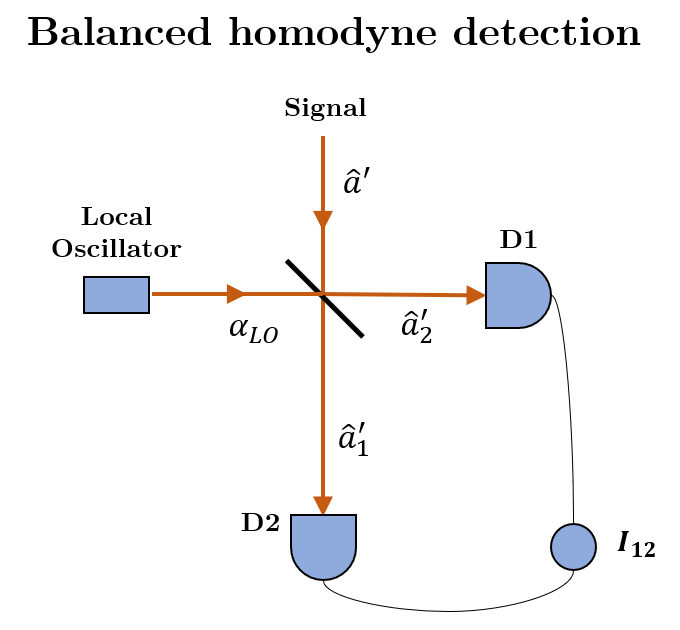
\includegraphics[width=0.6\linewidth]{BHD.png}
    \caption{General scheme for balanced homodyne detection.}
    \label{BHD}
\end{figure}

\begin{itemize}
    \item Because the local oscillator and the signal usually come from the same ``source'' laser, we may consider them to have a fixed phase relation.
    \item The local oscillator should be intense enough to be treated classically.
    \item Detectors are usually linear-response photodiodes
    \item The photocurrents are measured, processed and subtracted:
    \begin{equation}
        I_{12}=I_2-I_1
    \end{equation}
    \item We shall assume that photocurrents are proportional to the photon number $\hat n_1$ and $\hat n _2$ of each beam.
\end{itemize}

The photon numbers are given by:

\begin{equation}
    \hat n_1=\hat a^{'\dag}_1 \hat a^{'}_1
\end{equation}
\begin{equation}
    \hat n_2=\hat a^{'\dag}_2 \hat a^{'}_2
\end{equation}

And the mode operator, in turn, are given by:

\begin{equation}
    \hat a^{'}_1=\frac{1}{\sqrt{2}}(\hat a-\alpha_{LO})
\end{equation}

\begin{equation}
    \hat a^{'}_2=\frac{1}{\sqrt{2}}(\hat a+\alpha_{LO})
\end{equation}

Therefore, the photon number difference must be:

\begin{align*}
    \hat n_{21} &=\hat n_2-\hat n_1\\[0.3cm]
                &=\hat a^{'\dag}_2 \hat a^{'}_2-\hat a^{'\dag}_1 \hat a^{'}_1\\[0.3cm]
                &=\frac{1}{\sqrt{2}}(\hat a^{\dag}-\alpha^*_{LO})\frac{1}{\sqrt{2}}(\hat a-\alpha_{LO})+\frac{1}{\sqrt{2}}(\hat a^{\dag}+\alpha^*_{LO})\frac{1}{\sqrt{2}}(\hat a+\alpha_{LO})\\[0.3cm]
                &=\frac{1}{2}\Big[(\hat a^{\dag}-\alpha^*_{LO})(\hat a-\alpha_{LO})+(\hat a^{\dag}+\alpha^*_{LO})(\hat a+\alpha_{LO})\Big]\\[0.3cm]
                &=\alpha^*_{LO}\hat a+\hat a^{\dag}\alpha_{LO} \\[0.3cm]
\end{align*}

\todo[inline]{I'll skip it all the way to the next step.}

A few calculations will show that the measured quantity is indeed proportional to $\hat q_{\theta}$

\begin{equation}
    \hat n_{21}=2^{1/2}\abs{\alpha_{LO}}\hat q_{\theta}
\end{equation}

\begin{equation}
    \hat n_{21}=\frac{1}{\sqrt{2}}\abs{\alpha_{LO}}\big(\hat q \cos\theta+\hat p \sin\theta\big)
\end{equation}

\begin{equation}
    \Delta^2\hat n_{21}=\frac{1}{2}\abs{\alpha_{LO}}^2\big(\Delta^2\hat q \cos^2\theta+\Delta^2\hat p \sin^2\theta\big)
\end{equation}

\subsubsection{Spatial-temporal modes}

Let us represent the field by the operator $\hat E^{(+)}(\textbf{x},t)$ for the positive frequency component of the electric field:

\begin{equation}
    \Big( \frac{\partial^2}{\partial x^2}+\frac{\partial^2}{\partial y^2}+\frac{\partial^2}{\partial ^2}-\frac{1}{c^2}\frac{\partial^2}{\partial t^2}\Big)\hat E^{(+)}(\textbf{x},t)=0
\end{equation}

Evidently, we may represent the field operator in terms of a mode expansion:

\begin{equation}
    \hat E^{(+)}(\textbf{x},t)=\sum_{k}\omega_k^{1/2}\hat a_k v_k(\textbf{x})\exp(-i\omega_kt)
\end{equation}

And the spatial mode functions will be given by the Helmholtz equation:

\begin{equation}
    \Big( \frac{\partial^2}{\partial x^2}+\frac{\partial^2}{\partial y^2}+\frac{\partial^2}{\partial ^2}-\frac{\omega_k^2}{c^2}\Big)\hat v_k(\textbf{x})=0
\end{equation}

Such functions are supposed to be orthonormal, as well as form a complete set. Any superposition of field excitations can be written in terms of an expansion of such modes.

When we compute the total energy:

\begin{equation}
    \hat H=\int_{-\infty}^{\infty}\int_{-\infty}^{\infty}\int_{-\infty}^{\infty}\hat E^{(+)}(\textbf{x},t)^{\dag}\hat E^{(+)}(\textbf{x},t)dx\;dy\;dz
\end{equation}

The orthonormality will introduce delta functions to the integral, and the only remainders will be:

\begin{equation}
    \hat H=\sum_{k}\omega_k\hat a_k^{\dag}\hat a_{k}
\end{equation}

And the Heisenberg equation of motion:

\begin{equation}
    i\frac{\partial}{\partial t}\hat E^{(+)}(\textbf{x},t)=\comm{\hat E^{(+)}(\textbf{x},t)}{\hat H}
\end{equation}

\todo[inline]{continuar daqui}

\subsection{Detecção Homodina}

Na seção \ref{quatradure.amplitude}, definimos as amplitudes em quadratura de forma que a solução geral da equação de onda fica:

\begin{equation}
    \textbf{E}(\textbf{r},t)=E_0\textbf{p}(\textbf{r},t)\bigl[X_1(\textbf{r},t)\cos(\omega t)+X_2(\textbf{r},t)\sin(\omega t)\bigr]
\end{equation}

\begin{equation}
    \begin{cases}
        X_1(\textbf{r},t)=\alpha(\textbf{r},t)+\alpha^*(\textbf{r},t)\\
        X_2(\textbf{r},t)=i[\alpha(\textbf{r},t)-\alpha^*(\textbf{r},t)]\\
    \end{cases}
\end{equation}

\begin{figure}[H]
    \centering
    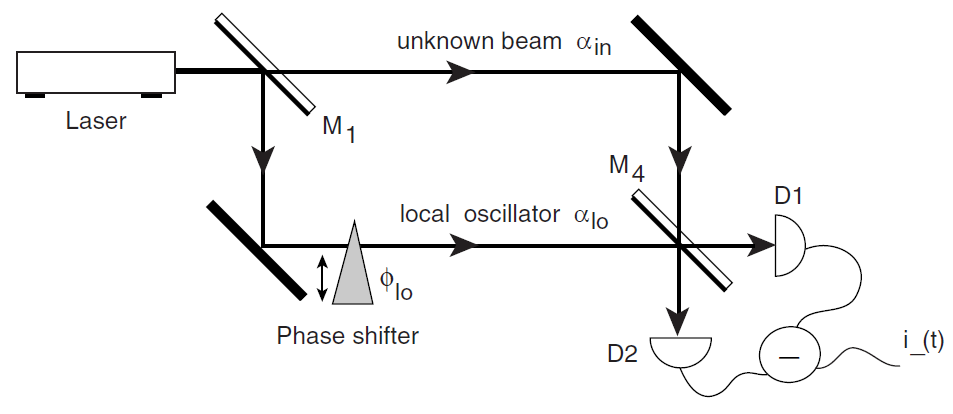
\includegraphics[width=1.0\linewidth]{homodyne detection.png}
    \caption{Montagem para detecção homodina.}
    \label{homodyne.detection}
\end{figure}

E vimos que essa notação é útil para escrever pequenas variações na amplitude e na fase de uma onda. Com efeito, podemos escrever os dois feixes da seguinte forma:

\begin{equation}
    \begin{cases}
        \alpha_{in}(t)=\alpha_{in}+\delta X_1_{in}(t)+i\delta X_2_{in}(t)\\
        \alpha_{lo}(t)=\big(\alpha_{lo}+\delta X_1_{lo}(t)+i\delta X_2_{lo}(t)\big)e^{i\phi_{lo}}
    \end{cases}
\end{equation}

Considerando que a intensidade do feixe do oscilador é muito maior que a do feixe medido $\alpha_{lo}^2\gg\alpha_{in}^2$. Nesse caso podemos supôr que toda a intensidade se deve ao oscilador, e que está igualmente distrubuída nos dois detectores:

\begin{equation}
    \abs{\alpha_{D1}}^2=\abs{\alpha_{D2}}^2=\frac{1}{2}\abs{\alpha_{lo}}^2
\end{equation}

Daí é fácil ver que:

\begin{equation}
    \begin{cases}
        \alpha_{D1}=\sqrt{1/2}\alpha_{lo}(t)+\sqrt{1/2}\alpha_{in}(t)\\
        \alpha_{D2}=\sqrt{1/2}\alpha_{lo}(t)-\sqrt{1/2}\alpha){in}(t)
    \end{cases}
\end{equation}

E a intensidade no detector 1:

\begin{equation}
    \abs{\alpha_{D1}}^2=\frac{1}{2}\Bigg[ \abs{\alpha_{lo}(t)}^2+\alpha_{lo}(t)\alpha^*_{in}(t)+\alpha_{in}(t)\alpha^*_{lo}+\abs{\alpha_{in}(t)}^2\Bigg]
\end{equation}

Fazendo algumas aproximações simples e resolvendo para a diferença entre os dois detectores:             

\begin{equation}
    i_{-}(t)\approx 2\alpha_{lo}\big(\delta X_1_{in}(t)\cos(\phi_{lo})+i\delta X_2_{in}(t)\sin(\phi_{lo})\big)
\end{equation}




\subsubsection{Inefficiencies in homodyne detection}































%===============================================================================================================================================================================================================================================================================================================================================================================================================================================================

\chapter{Photons}

\section{Photon Statistics}

\subsection{Introduction}

In this section, we are interested in studying the three types of photon statistics that can occur for a photon stream: (1) Poissonian, (2) super-Poissonian, (3) sub-Poissonian. The first two types of stream are consistent with the predictions of the classical theory of light. On the other hand, sub-Poissonian streams requires a quantum theory, and provides direct confirmation of the photon nature of light.

If you place a photon source in front of a photo-detector, like a Photo-Multiplier Tube (PMT) or an Avalanche Photo-Diode (APD), the \textbf{output count rate will fluctuate around an average value}. The average count rate will be determined by the intensity of the light, but the measured count rate will fluctuate between measurements.

If we were ignorant of limitations in the measurement process, we might immediately use this as ``proof'' that the stream of photons is made up of discrete energy packets. In this case, there would be a perfect correspondence between the statistical properties of the fluctuations in the count rate, and the intrinsic statistical properties of the stream of these packets.

In practice, however, such statistical properties were first attributed to the \textbf{nature of the photo-detection process} and only later to the \textbf{intrinsic photon statistics of the light beam}. Only a small number of experiments actually require a treatment of photon statistics, and most can be handled by a semi-classical approach, in which the light is treated classically, and quantization is introduced via the photoelectric effect inside the photo-detector.

\subsubsection{Photon Counting Statistics}

Let us define a few fundamental quantities in photon counting statistics. First, the \textbf{photon flux} for a monochromatic beam:

\begin{equation}
    \Phi=\frac{IA}{\hbar \omega}=\frac{P}{\hbar \omega}
\end{equation}

Which, intuitively, is measured in photons per second. If we adjust this by a dimensionless coefficient $\eta$ referring to the \textbf{efficiency of the counter}, we can get the number of actual counts in a given detection time interval $T$:

\begin{equation}
    N(T)=\eta\Phi T
\end{equation}

And finally, the average \textbf{count rate} $R(T)$ in the time interval will be:

\begin{equation}
    R=\frac{N}{T}=\eta\Phi
\end{equation}

Obviously, all of these are average quantities. What does it mean to say that a given beam emits, say, three billion photons per second? Ideally, it would mean that if we let the emission run for exactly one second, we would have a $c \Delta t=3\times10^8$ meters-long beam containing three billion equally spaced photons.

If we set a count time of $1 ns$, that means we should be measuring one billionth of the total number of photons in the beam, which equals three photon. Equivalently, we could say that a $c \Delta t=30$ centimeters-long beam should contain three photons.

In practice, however, if the detection time-interval is indeed set at $1 ns$, the actual measured number of photons will be a sequence of numbers with a mean close to $3$ and a certain variance.

We close this section by concluding that ``although the average photon flux can have a well-defined value, the photon number on short time-scales fluctuates due to the discrete nature of the photons''. These fluctuations are described by the \textbf{photon statistics of light}.

\subsubsection{Coherent Light: Poissonian Statistics}\label{poissonian.statistics.with.photons}

We are now interested in showing that perfectly coherent light of constant intensity has Poissonian photon statistics.

The average number of photons in a beam of length $L$ is:

\begin{equation}
    \bar{n}=\Phi \frac{L}{c}
\end{equation}

$L$ is divided up into $N$ equally sized segments. $N$ is large enough so that finding a photon in any particular segment is very unlikely, and finding two photons in the same segment in virtually impossible.

If we ask: ``how many ways are there to choose $n$ segments to place photons in among a total set of $N$ segments'', the answer will be:

\begin{equation}
    \binom{N}{n} = \frac{N!}{n!(N-n)!}
\end{equation}

And the probability that any given segment will be filled is given by:

\begin{equation}
    p=\frac{\bar{n}}{N}
\end{equation}

Therefore we arrive at the following binomial distribution for the probability that $n$ photons will be found in a beam of length $L$ containing $N$ segments:

\begin{equation}
    P(n)=\frac{N!}{n!(N-n)!} p^n(1-p)^{N-n}
\end{equation}

If we take $N\rightarrow\infty$:

\begin{equation}
    \lim_{N\rightarrow\infty}\big[P(n)\big]=\frac{N!}{n!(N-n)!} \Big(\frac{\bar{n}}{N}\Big)^n\Big(1-\frac{\bar{n}}{N}\Big)^{N-n}
\end{equation}

\begin{equation}
    \lim_{N\rightarrow\infty}\big[P(n)\big]=\frac{\bar{n}^n}{n!}\Big(\frac{N!}{(N-n)!N^n}\Big)\Big(1-\frac{\bar{n}}{N}\Big)^{N-n}
\end{equation}

Stirling's formula (or intuition) can be used to show that the fraction in the first parenthesis goes to one.

\begin{equation}
    \lim_{N\rightarrow\infty}\big[P(n)\big]=\frac{\bar{n}^n}{n!}\Big(1-\frac{\bar{n}}{N}\Big)^{N-n}
\end{equation}

By fundamental exponential limit:

\begin{equation}
  \lim_{N\rightarrow\infty}\Big(1-\frac{\bar{n}}{N}\Big)^N=e^{-\bar{n}}  
\end{equation}

\begin{equation*}
\lim_{N\rightarrow\infty}\Big(1-\frac{\bar{n}}{N}\Big)^N=\lim_{N\rightarrow\infty}\frac{\Big(1-\frac{\bar{n}}{N}\Big)^N}{\Big(1-\frac{\bar{n}}{N}\Big)^{\bar{n}}}=  \lim_{N\rightarrow\infty}\Big(1-\frac{\bar{n}}{N}\Big)^{N-\bar{n}}
\end{equation*}

Since the denominator clearly goes to one in the limit. We conclude that the photon statistics for a coherent light with constant intensity are given by:

\begin{equation}
    \boxed{P(n)=\frac{\bar{n}^n}{n}e^{-\bar{n}}}
\end{equation}

Which is a Poisson distribution. This result is expected, given that Poisson distributions generally describe random processes that can only return integer values. In this case, the randomness comes from the need to split the ``continuous'' beam into discrete energy packets with an equal probability of finding the energy packet at any given sub-interval.

A fundamental property of Poisson distributions is that the variance is equal to the mean value:

\begin{equation}
    (\Delta n)^2=\bar{n}
\end{equation}

Therefore, the standard deviation is:

\begin{equation}
    \Delta n=\sqrt{\bar{n}}
\end{equation}

That means the standard deviation will increase with the square root of the mean: the relative size of the fluctuations becomes smaller as the expected value is higher.

\begin{figure}[H]
    \centering
    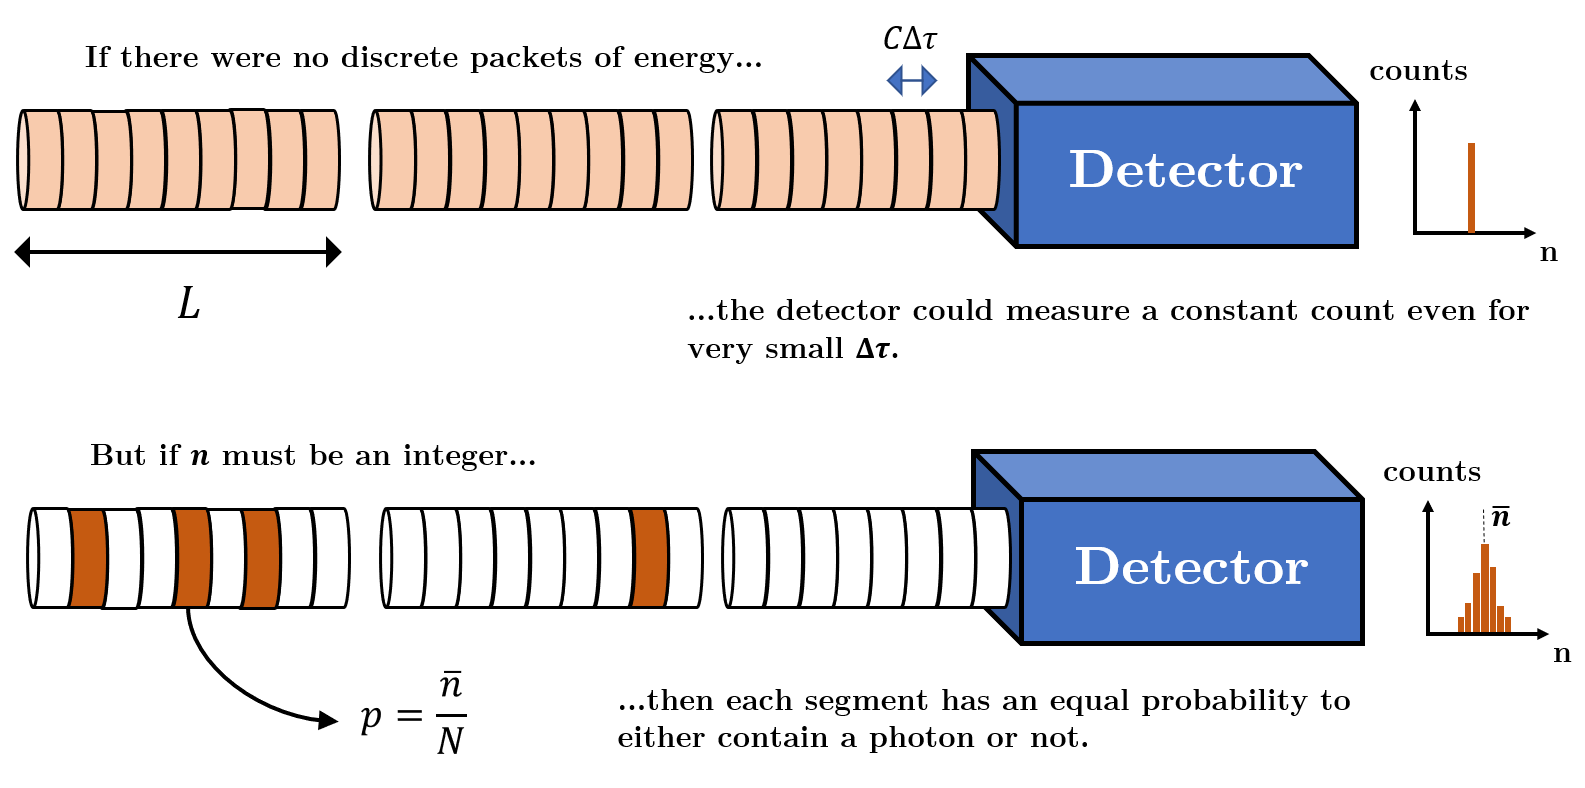
\includegraphics[width=1\linewidth]{detector.statistics.png}
    \caption*{}
\end{figure}

We may now run a Monte Carlo simulation in order to both verify and understand the proposed model. We will assign an expected value $\bar{n}$ for the number of photons in a beam (in the lab, this amounts to a choice in photon flux and detection time). Each beam is divided into a very high number $N$ of segments, which may be occupied by a photon with probability $p=\bar{n}/N$.

Finally, a Monte Carlo algorithm is implemented to simulate such beams using pseudo-random numbers. For the data in Figure \ref{poisson.detection}, we consider $10^4$ beams being fed into the detector in order to make a histogram of the number of photons measured. The dotted line indicates the analytical result for a Poisson Distribution with mean equal to $\bar{n}$

\begin{figure}[H]
    \centering
    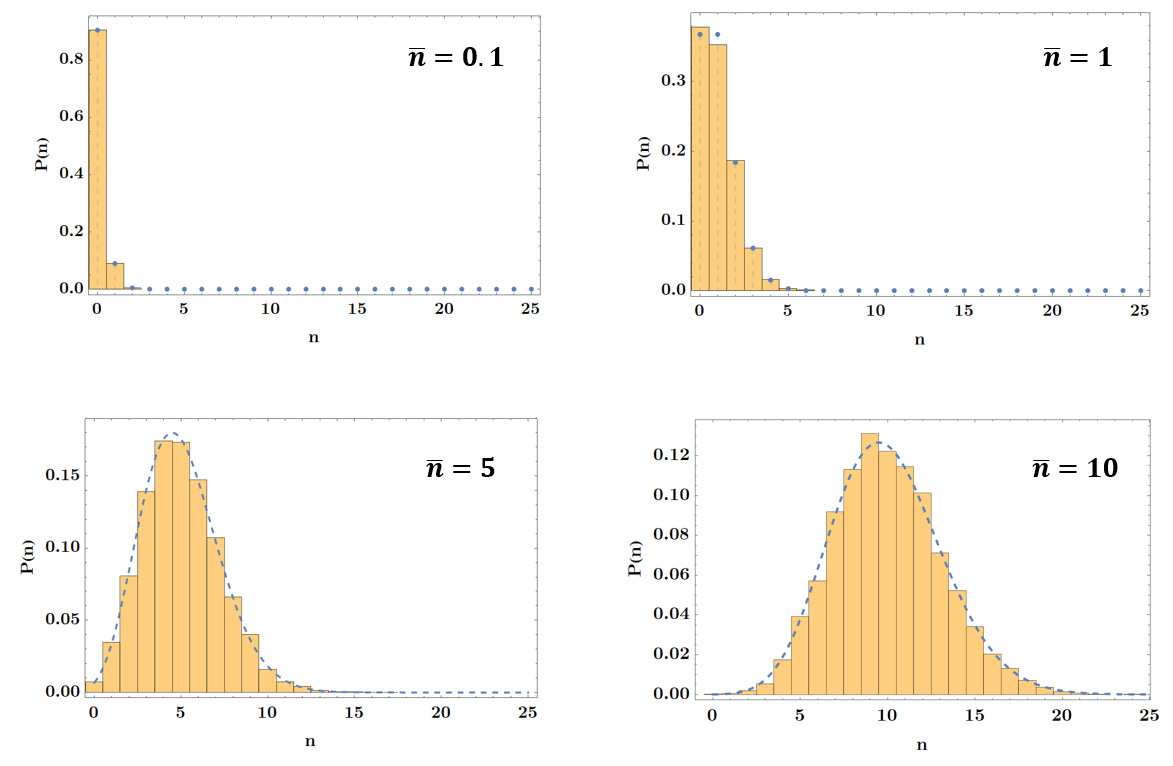
\includegraphics[width=1\linewidth]{poisson.detection.png}
    \caption{Monte Carlo simulation results for different expected values for the number of photons in a beam. Dotted lines/points are the exact results for the corresponding Poisson distribution.}
    \label{poisson.detection}
\end{figure}

\subsection{Classification of Light by Photon Statistics}

We are now motivated to classify light in to three statistical categories, according to how the standard deviation of the photon number relates to the mean:

\begin{equation}
    \begin{cases}
        \Delta n<\sqrt{\bar{n}}\;\;\;\;\text{sub-Poissonian}\\
        \Delta n=\sqrt{\bar{n}}\;\;\;\;\text{Poissonian}\\
        \Delta n>\sqrt{\bar{n}}\;\;\;\;\text{super-Poissonian}\\
    \end{cases}
\end{equation}

We have shown that the \textbf{Poissonian case occurs for a perfectly coherent beam with constant intensity}. Which, from a classical perspective, is the most stable type of light conceivable.

In order to obtain super-Poissonian light, it is enough to have the intensity vary in time. For sub-Poissonian light, however, \textbf{there is no classical understanding}.

\subsubsection{Super-Poissonian light}

As an example of super-Poissonian statistics, let us consider \textbf{thermal light}. Each mode of thermal emission can be modeled as a harmonic oscillator:

\begin{equation}
    E_n=\Big(n+\frac{1}{2}\Big)\hbar\omega
\end{equation}

\todo[inline]{A quantum optical interpretation would clearly claim that $n=$ the number of photons in the mode. What is the classical interpretation, though? Would $n$ simply be a mode number, as in waves propagating in strings and tubes?}

Applying the canonical ensemble formalism, we can define ``Boltzmann weights'' to the number of photons contributing to the $\omega$-mode.

\begin{equation}
    P(n)=\frac{\exp{-E_n/k_BT}}{\sum_{n=0}^{\infty}\exp{-E_n/k_BT}}
\end{equation}

Starting from this equation, simple manipulations will lead to the following:

\begin{equation}
    P(n)=\frac{1}{\bar{n}+1}\Big(\frac{\bar{n}}{\bar{n}+1}\Big)^n
\end{equation}

Which is the \textbf{Bose-Einstein} distribution, whose variance is given by $(\Delta n)^2=\bar{n}+\bar{n}^2$. Clearly, it is always broader than a Poisson distribution. This distributions would be observed for single-mode black-body radiation.

A second example of super-Poisson (or at most Poissonian) statistics is \textbf{Chaotic Light}. Skipping a few steps, its count rate in a detection interval $T$ is given by:

\begin{equation}
    W(T)=\int_{t}^{t+T}\eta \Phi(t')dt'
\end{equation}

And the variance is given by:

\begin{equation}
    (\Delta n)^2 = \langle W(T) \rangle + \langle \Delta W(t)^2 \rangle
\end{equation}

Clearly, if the detection interval is much larger than the coherence time $\tau_c$, the second term in the RHS of the expression for the variance will be null, since fluctuations in the beam intensity will be unnoticeable. In this case, the chaotic light will display Poissonian statistics, as $\langle W(T) \rangle=\bar{n}$. If the detection interval is of the same order as $\tau_c$, then the second term in the RHS will be greater than zero, and we'll have super-Poissonian statistics.

\subsubsection{Sub-Poissonian light}

sub-Poissonian light is more stable than perfectly coherent constant-intensity light. There is no classical equivalent to sub-Poissonian light. It is, therefore, a demonstration of the quantum nature of light.

If a beam of light rigorously emits single photons in equal $\Delta t$ time limits, the registered photocount for a detection interval $T$ is:

\begin{equation}
    N=\Int\Big(\eta\frac{T}{\Delta t}\Big)
\end{equation}

Which would always yield the same measurement $N=\bar{n}$, with zero standard deviation. Such $\Delta n =0$ states are called \textbf{photon number states}, which are the purest forms of sub-Poissonian light.

Sub-Poissonian light is extremely fragile, in the sense that its statistics are easily degraded by all forms of inefficiency. A convenient way to model \textbf{random sampling} processes during detection is through beam splitters (Section \ref{beam.splitter.section}). Such processes include inefficient collection of the emitted light by the detector, optical losses due to reflection, scattering and absorption, and imperfect quantum efficiencies at the detectors.


\subsection{Theory of Photodetection}

\subsubsection{Semi-classical theory of photodetection}

It is possible to explain the Poissonian count statistics observed when detecting light without any reference to photons. As we wrote in the beginning of this chapter, this photon-free explanation chronologically precedes the ``random-walk'' explanation which we presented in Section \ref{poissonian.statistics.with.photons}.

In our original explanation, the Poisson distribution appeared once we partitioned a light beam with an average total photon number $\bar{n}$ (determined by photon flux and detection interval) into $N$ pieces. $N$ was large enough so that each piece could only contain either no photons, or one photon. The probability for an ``occupied'' site was then independent for each, and given by $p=\bar{n}/N$. We showed, both analytically and via numerical simulation, that this leads to a Poisson distribution.

The semi-classical approach, instead of quantizing the photons in the light beam, outsources the quantization to the photoelectric emission in the detector. In this picture, a light beam with a certain intensity $I$ aimed at a detector during a time interval $\Delta t$ has a probability $\varepsilon$ of leading to the emission of a photoelecton.

\begin{equation}
    P(1;t,t+\Delta t)=\varepsilon I(t)\Delta t
\end{equation}

By making $\Delta t$ short enough, we can virtually ensure that $P(2;t,t+\Delta t)=0$. Furthermore, it is now enough to simply consider that photoelectric emissions in different time intervals are independent, and we will arrive at the same Poisson distribution as before. (Obs.: demonstrating that these considerations do indeed lead to a Poisson distribution is not hard, but it is long, so I will skip it here).

If we make the intensity change in time, all we can get is super-Poissonian statistics. Therefore \textbf{a semi-classical theory of photodetection} is unable to explain sub-Poissonian statistics. Such results can \textbf{only} be explained by a quantum treatment of light detection.

\subsubsection{Quantum theory of photodetection}

The variance $(\Delta N)^2$ in the photocount number measured by a detector, and the corresponding variance $(\Delta n)^2$ in the number of incident photons are related by:

\begin{equation}
    (\Delta N)^2=\eta^2(\Delta n)^2+\eta(1-\eta)\bar{n}
\end{equation}

\todo[inline]{This equation is demonstrated on page 273 in Loudon's "The Quantum Theory of Light" \cite{Loudon448s}. I can't really understand  it yet, though. For now, I will just state the result and work with it.}

It is easy to see that:

\begin{equation}
    \eta=\frac{\bar{N}}{\bar{n}}
\end{equation}

\begin{enumerate}
    \item If the detector is perfectly efficient ($\eta=1$), then all of the photocount fluctuations are due to the photon number fluctuations ($\Delta N = \Delta n$).
    \item  If the incident light has Poissonian statistics, then $\Delta n=\bar{n}$:
    \begin{equation*}
        (\Delta N)^2=\eta^2(\Delta n)^2+\eta(1-\eta)\bar{n}\;\;\;\Rightarrow\;\;\;(\Delta N)^2=\eta^2\bar{n}^2+\eta(1-\eta)\bar{n}=\eta\bar{n}=\bar{N}
    \end{equation*}
    That means the photocount will also give a Poisson distribution.
    \item If $\eta\ll1$, the quadratic terms in $\eta$ will be negligible, and once again:
    \begin{equation*}
        (\Delta N)^2=\eta^2(\Delta n)^2+\eta(1-\eta)\bar{n}\;\;\;\Rightarrow\;\;\;(\Delta N)^2=\eta\bar{n}=\bar{N}
    \end{equation*}
\end{enumerate}

From these observations, we conclude that low efficiency detectors will lead to Poissonian distributions, regardless of the statistical nature of the incoming light beam. Therefore, in order to observe sub-Poissonian results, high-efficiency detector are necessary.

\subsection{Shot Noise in Photodiodes}

The working principle behind photodiodes is well-known:

\begin{displayquote}
    ``If a reverse-biased \textit{pn} junction is exposed to incident light, the photons impacting the junction cause covalent bonds to break, and thus electron-hole pairs are generated in the depletion layer. The electric field inside the depletion region then sweeps the liberated electrons to the $n$-side and the holes to the $p$-side, giving rise to a reverse current across the junction. This current, known as the photocurrent, is proportional to the intensity of the incident light.'' (Sedra, Adel S. \textit{Microelectronic Circuits})
\end{displayquote}

Single photon counting detectors would be easily saturated by all but a few very low-flux beams ($~10^6 photons/s$). In order to detect high flux light beams, photodiode detectors are usually employed. 

The generated photocurrent is given  by:

\begin{equation}
    i=\eta e \Phi=\eta e \frac{P}{\hbar\omega}
\end{equation}

The fluctuations in the photon numbers will translate to fluctuations in the photocurrent according to the quantum efficiency $\eta$. Such fluctuations will manifest as noise in the photocurrent. Clearly, we may write the photocurrent as:

\begin{equation}
    i(t)=\langle i \rangle + \Delta i(t)
\end{equation}

The average value of the fluctuations must be zero. We may define the \textbf{noise power} as:

\begin{equation}
    P_{noise}(t)=(\Delta i(t))^2R_L
\end{equation}

Where $R_L$ is a load resistor connected to the photodiode. If we let a single-mode, perfectly coherent laser illuminate a photodiode, the photon electron statistics should reflect the Poissonian statistics:

\begin{equation}
    (\Delta N)^2=\langle N \rangle
\end{equation}

Given that the photocurrent is proportional to the number of photoelectrons, its variance also obeys:

\begin{equation}
    (\Delta i)^2 \propto \langle i \rangle
\end{equation}

Taking the Fourier transform of $i(t)$ and then measuring the variance of the current fluctuations within a frequency bandwidth $\Delta f$:

\begin{equation}
    (\Delta i)^2=2e\Delta f\langle i \rangle
\end{equation}

And the expression for the noise power follows:

\begin{equation}
    (\Delta i)^2=2eR_L\Delta f\langle i \rangle
\end{equation}

One way to demonstrate this is:

\begin{equation}
    i=\eta e \Phi=\frac{Ne}{\Delta t}  \;\;\;\Rightarrow\;\;\; (\Delta i)^2=\frac{(\Delta N)^2e^2}{\Delta t^2}= \frac{\bar{N}e^2}{\Delta t^2}
\end{equation}

And the mean number of photoeletrons is itself related to the mean photocurrent:

\begin{equation}
    (\Delta i)^2= \frac{\bar{i}\Delta t}{e}\frac{e^2}{\Delta t^2}=\frac{\bar{i}e}{\Delta t}
\end{equation}

Finally, let us write the \textbf{bandwidth} as $\Delta f=1/2\Delta t$:

\begin{equation}
    \boxed{(\Delta i)^2=2e\Delta f \langle i \rangle}
\end{equation}

This expression, which relates the variance of the photocurrent to its mean, defines the \textbf{shot noise} for the photocurrent. Let us point out two important characteristics:

\begin{enumerate}
    \item Variance is proportional to mean value;
    \item Noise spectrum is independent of frequency. That is, if we ignore the maximum frequency determined by the detectors response time.;
\end{enumerate}

\todo[inline]{It is still not clear why the bandwidth is defined as $B=1/2\Delta t$.}

Most classical noise sources are limited to lower frequencies. For its frequency-independence, shot noise will usually be the only noise observable at high frequencies. Therefore, in a frequency domain graph of noise power, the data will form a horizontal asymptote near the \textbf{shot noise limit}, reflecting the fundamental photon statistics.

\begin{figure}[H]
    \centering
    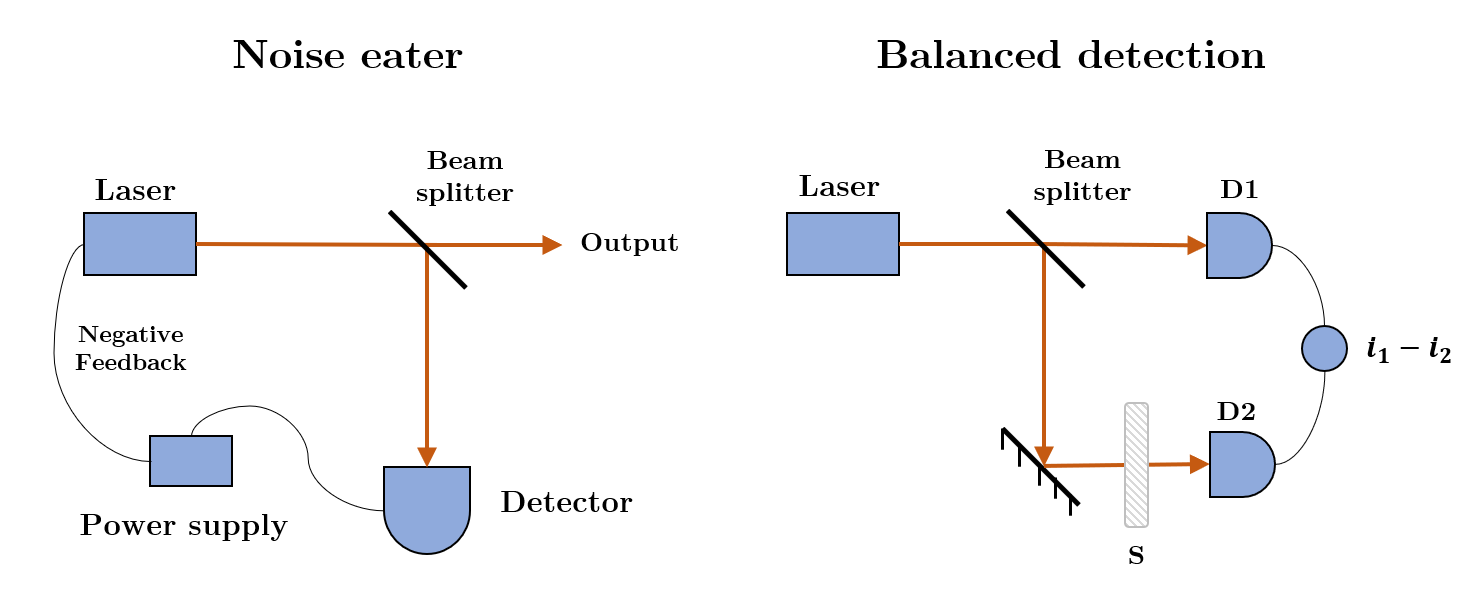
\includegraphics[width=1.0\linewidth]{balanced detection and noise eater.png}
    \caption{The noise eater monitors the power output of the laser and uses it to control the power supply in a negative feedback loop. The balanced detection scheme cancels classical noise by subtracting the two currents.}
    \label{noise.eater.and.balanced.detection}
\end{figure}


Figure \ref{noise.eater.and.balanced.detection} show two schemes for minimizing classical noise. Neither are able to cancel \textbf{shot noise}, which is intrinsic to the light.

Therefore, \textbf{shot noise imposes a limit to the minimum signal to noise ratio that can be achieved}.

\begin{displayquote}
    ``The only way to beat the shot noise limit is to use non-classical light sources with sub-Poissonian photon statistics.''
\end{displayquote}

\subsection{Observation of sub-Poissonian photon statistics}

The most general scheme for producing sub-Poissonian light is to first generate a sub-Poissonian current source, and then use a high-efficiency emitter to produce light with the same statistical properties.

Conceptually speaking producing an evenly spaced beam of electrons should be easier than doing the same for photons. First, because electrons repel each other through Coulomb forces. Second, because the Pauli exclusion principle forbids electrons to occupy the same quantum state in a given quantum system. Photons possess neither of those properties.

One rudimentary example of sub-Poissonian electron emission occurs in a Frank-Hertz tube. It consists of a previously evacuated metal tube, filled with mercury atoms, and two electrodes, which emit electrons through thermal emission.

In turn, as is well known from the famous Frank-Hertz experiment, these electrons can collide inelastically  with mercury atoms when their energies are multiples of $~4.8 eV$. In this case, an electron will be excited in a  mercury atom, and will later emit a photon.

The presence of \textbf{space charge} (an electron ``cloud'') accumulated around the anode will regularize the electron flow, so that the electron statistics are sub-Poissonian.

\todo[inline]{Most likely this has something to do with space-charge limited current. I'm still not sure how this is better than thermal emission, though.}

The same principle can be applied to obtain sub-Poissonian photon statistics from solid-state emitters, such as LEDs.

A convenient way to measure the \textbf{shot-noise reduction} in a sub-Poissonian source is through the \textbf{Fano factor}:

\begin{equation}
    F_{Fano}=\frac{\text{measured noise}}{\text{shot noise limit}}
\end{equation}



\section{Coherent States and Squeezed Light}

\subsection{Light waves as classical harmonic oscillators}

Let us consider a stationary wave, polarized in the $x$-direction inside of an empty cavity of length $L$. The equation for the electric field is:

\begin{equation}
    \mathcal{E}_x=\mathcal{E}_0\sin(kz)\sin(\omega t)
\end{equation}

If we multiply this by $1/c^2=\mu_0\epsilon_0$ and take its time derivative:

\begin{equation}
    \mu_0\epsilon_0\frac{\partial{\mathcal{E}_x}}{\partial t}=\omega\mu_0\epsilon_0\mathcal{E}_0\sin(kz)\cos(\omega t)
\end{equation}

According to Equation \ref{curlBvac}, this should be equal to the magnetic field curl. Since $\textbf{B}=B_y\hat{y}$, that will give minus the $z$-derivative of $B_y$, pointing in the same direction as the electric field:

\begin{equation}
    -\frac{\partial B_y}{\partial z}=\omega\mu_0\epsilon_0\mathcal{E}_0\sin(kz)\cos(\omega t)
\end{equation}

Integrating with respect to $z$:

\begin{equation}
    B_y=\frac{\omega}{k}\mu_0\epsilon_0\mathcal{E}_0\cos(kz)\cos(\omega t)
\end{equation}

Since $c=\omega/k$:

\begin{equation}
    B_y=c \Big(\frac{1}{c^2}\Big)\mathcal{E}_0\cos(kz)\cos(\omega t)
\end{equation}

Defining $B_0=\mathcal{E}_0/c$:

\begin{equation}
    B_y=B_0\cos(kz)\cos(\omega t)
\end{equation}

Clearly, $B_y$ and $\mathcal{E}_y$ have a $\pi/2$ phase difference. It is well known that a standing wave of frequency $\omega$ and wavenumber $k$ corresponds to a combination of two propagating waves with the same frequency $\omega$ and wavenumber $k$, and half the amplitude, travelling in opposite directions. There is a $\pi/2$ phase difference between combining them with a sum, and with a subtraction.

If we consider the energy density of the electromagnetic wave:

\begin{equation}
    U=\frac{1}{2}\Bigg(\epsilon_0\mathcal{E}^2+\frac{1}{\mu_0}B^2\Bigg)
\end{equation}

Integrating the energy density inside the cavity (just take an integral from $z=0$ to $z=L$, multiplied by the cross section A, $V=AL$) with boundary conditions $\mathcal{E}(z=0)=\mathcal{E}(z=L)=0$:

\begin{equation}
    E_{el}=\frac{1}{4}\epsilon_0V\mathcal{E}_0^2\sin^2(\omega t)
\end{equation}

\begin{equation}
    E_{mag}=\frac{1}{4\mu_0}VB_0^2\cos^2(\omega t)
\end{equation}

Thus the total energy is:

\begin{equation}
    \boxed{E=\frac{V}{4}\Bigg(\epsilon_0\mathcal{E}_0^2\sin^2(\omega t)+\frac{B_0^2}{\mu_0}\cos^2(\omega t)\Bigg)}
\end{equation}

If we attempt to write this same expression as:

\begin{equation}
    E=\frac{1}{2}\Big(p^2+\omega^2q\Big)
\end{equation}

Then we can find definitions for $p$ and $q$:

\begin{equation}
    \begin{cases}
        p(t)=\Big(\frac{V}{2\mu_0}\Big)^{1/2}B_0\cos(\omega t)=\Big(\frac{\epsilon_0V}{2}\Big)^{1/2}\mathcal{E}_0\cos(\omega t)\\[0.3cm]
        q(t)=\Big(\frac{\epsilon_0V}{2\omega^2}\Big)^{1/2}\mathcal{E}_0\sin(\omega t)
    \end{cases}
\end{equation}

Once we have done that, there is a clear analogy between how energy is distributed among electric and magnetic field in a electromagnetic wave, and how it is distributed among kinetic and potential energy in a classical harmonic oscillator.

\subsection{Field quadratures}

Let us right the same stationary wave as before, but in a more general case, including a phase factor:

\begin{equation}
    \mathcal{E}_x(z,t)=\mathcal{E}_0\sin(kz)\sin(\omega t+\varphi)
\end{equation}

\begin{equation}
    \mathcal{E}_x(z,t)=\mathcal{E}_0\sin(kz)(\sin{\omega t}\cos{\phi}+\cos{\omega t}\sin{\phi})
\end{equation}

If we multiply and divide by $(\epsilon_0V/4\hbar\omega)^{1/2}$:

\begin{equation*}
    \mathcal{E}_x(z,t)=
    \Big(\frac{4\hbar\omega}{\epsilon_0V}\Big)^{1/2}
    \sin(kz)
    \Bigg[
    \Big(\frac{\epsilon_0V}{4\hbar\omega}\Big)^{1/2} \mathcal{E}_0\sin{\omega t}\cos{\phi}
    +
    \Big(\frac{\epsilon_0V}{4\hbar\omega}\Big)^{1/2} \mathcal{E}_0\sin{\phi}\cos{\omega t}
    \Bigg]
    \label{pre.quadrature}
\end{equation*}

The multiplication by $(\epsilon_0V/4\hbar\omega)^{1/2}$ makes the terms inside the square brackets dimensionless, since it has units of inverse electric field ($m/V$).

We can now write Equation \ref{pre.quadrature} as:

\begin{equation*}
    \mathcal{E}_x(z,t)=
    \Big(\frac{4\hbar\omega}{\epsilon_0V}\Big)^{1/2}
    \sin(kz)
    \Big[
    X_1(t)\cos{\phi}
    +
    X_2(t)\sin{\phi}
    \Big]
    \label{pre.quadrature}
\end{equation*}

Where $X_1$ and $X_2$ are the \textbf{field quadrature amplitudes}:

\begin{equation}
    \begin{cases}
        X_1(t)= \Big(\frac{\epsilon_0V}{4\hbar\omega}\Big)^{1/2} \mathcal{E}_0\sin{\omega t}\\[0.3cm]
        X_2(t)=\Big(\frac{\epsilon_0V}{4\hbar\omega}\Big)^{1/2} \mathcal{E}_0\cos{\omega t}
    \end{cases}
    \label{field.quad.amplitudes.equations}
\end{equation}


They should seem familiar to the definitions we presented for generalized position and momentum:

\begin{equation}
    \begin{cases}
        p(t)=\Big(\frac{\epsilon_0V}{2}\Big)^{1/2}\mathcal{E}_0\cos(\omega t)\\[0.3cm]
        q(t)=\Big(\frac{\epsilon_0V}{2\omega^2}\Big)^{1/2}\mathcal{E}_0\sin(\omega t)
    \end{cases}
\end{equation}

It's worth remembering that we defined this so as to obtain an analogy between energy distribution in light (among electric and magnetic field) and energy distribution in a classical harmonic oscillator (among kinetic and potential energy). The electric field "behaves" like generalized momentum, and the magnetic field like generalized position.

We need only make a few adjustments in the coefficients:

\begin{equation}
    \boxed{\begin{cases}
        X_1(t)= \big(\frac{\omega}{2\hbar}\big)^{1/2}q(t)\\[0.3cm]
        X_2(t)=\big(\frac{1}{2\hbar\omega}\big)^{1/2}p(t)
    \end{cases}}
\end{equation}

What have we done so far?

\begin{itemize}
    \item We have shown that the electric and magnetic fields in a standing electromagnetic wave behave like position and momentum in a harmonic oscillator. Their formalisms can become identical under simple transformations: \textbf{the two systems have the same physics.}
    \item We have shown that all of the time dependence in the electric field can be expressed in terms of field quadrature amplitudes.
    \item The two former items can be used to make a final bridge, relating the field quadratures to the position and momentum coordinates.
\end{itemize}

\subsection{Light as a Quantum Harmonic Oscillator}

We know how to treat light as a harmonic oscillator. We know how to quantize a harmonic oscillator. We should now be able to quantize light. In Section \ref{quantum.harmonic.oscillator}, we reviewed the basic formalism for the quantum harmonic oscillator.

If we multiply the uncertainties (standard deviations) of both field quadratures:

\begin{equation}
    \Delta X_1\Delta X_2=\Big(\frac{\omega}{2\hbar}\Big)^{1/2}\Delta q\Big(\frac{1}{2\hbar\omega}\Big)^{1/2}\Delta p
\end{equation}

\begin{equation}
    \Delta X_1\Delta X_2=\Big(\frac{1}{2\hbar}\Big)\Delta q\Delta p
\end{equation}

The total equivalence between the generalized $q$ and $p$ presented here and $x$, $p_x$ for the harmonic oscillator is achieved by making $q=\sqrt{m}x(t)$ and $p=(1/\sqrt{m})p_x$. These mass-related coefficients will cancel out in the expression above, so we might as well write:

\begin{equation}
    \Delta X_1\Delta X_2=\Big(\frac{1}{2\hbar}\Big)\Delta x\Delta p_x
\end{equation}

But the uncertainty principle dictates:

\begin{equation}
    \Delta x \Delta p_x>=\frac{\hbar}{2}
\end{equation}

Therefore:

\begin{equation}
    \boxed{\Delta X_1 \Delta X_2>=\frac{1}{4}}
\end{equation}

\begin{center}
\fbox{
    \parbox{\textwidth}{
        \centering The field quadratures are \textbf{subject to quantum uncertainty} in exact analogy to the quantum uncertainty of the position and momentum of a harmonic oscillator. Quantum theory introduces an intrinsic uncertainty into the amplitude and phase of the wave.
    }
}
\end{center}

We also know that the energy in a quantum harmonic oscillator relates to the number of photons via:

\begin{equation}
    E=\Big(n+\frac{1}{2}\Big)\hbar\omega
\end{equation}

Therefore, even when no photons are excited ($n=0$), the energy in the oscillator is $(1/2)\hbar\omega$. Such energy can be understood as the result of the so called \textbf{vacuum field}. Whose magnitude $\mathcal{E}_{vac}$ can be evaluated by considering and evacuated optical cavity:

\begin{equation}
    E=2\int{\frac{1}{2}\epsilon_0\mathcal{E}^2_{vac}dV}=\frac{1}{2}\hbar\omega
\end{equation}

Since the vacuum field is the same across the volume:

\begin{equation}
    \mathcal{E}_{vac}=\Big(\frac{\hbar\omega}{2\epsilon_0V}\Big)^{1/2}
\end{equation}

Clearly, the uncertainties for the two quadratures in the vacuum field are:

\begin{equation}
    \Delta X_1^{vac}=\Delta X_2^{vac}=\frac{1}{2}
\end{equation}

Which classifies it as a \textbf{minimum uncertainty state}.

\subsection{Coherent States}

A coherent state $\ket{\alpha}$ is the specific quantum state of the quantum harmonic oscillator. In quantum optics, it refers to a state of the quantized electromagnetic field. 

Let us consider a coherent state, defined as a dimensionless complex number:

\begin{equation}
    \alpha=X_1+iX_2
\end{equation}

\begin{equation}
    \alpha=\abs{\alpha}e^{i\phi}
\end{equation}

A coherent state is a \textbf{minimum uncertainty state}, or a \textbf{displaced vacuum state}, therefore:

\begin{equation}
    \Delta X_1=\Delta X_2=\frac{1}{2}
\end{equation}

\todo[inline]{it seems as if this could be a defining property of coherent states. Have to look into it later}

Once again, let us define the amplitude $\abs{\alpha}$ as a dimensionless correspondent of the field amplitude $\mathcal{E}_0$:

\begin{equation}
    \abs{\alpha}=\Big( \frac{\epsilon_0V}{4\hbar\omega} \Big)^{1/2}\mathcal{E}_0
\end{equation}

We saw that the total energy in the electromagnetic wave is:

\begin{equation}
    E_{\text{classical}}=\frac{V}{4}\Bigg(\epsilon_0\mathcal{E}_0^2\sin^2(\omega t)+\frac{B_0^2}{\mu_0}\cos^2(\omega t)\Bigg)
\end{equation}

Given $B_0=c\mathcal{E}_0$ and $c=1/\sqrt{\epsilon_0\mu_0}$:

\begin{equation}
    E_{\text{classical}}=\frac{\epsilon_0V}{4}\mathcal{E}_0^2\Big(\sin^2(\omega t)+\cos^2(\omega t)\Big)=\frac{\epsilon_0V}{4}\mathcal{E}_0^2
\end{equation}

Which relates to the magnitude $\abs{\alpha}$ by:

\begin{equation}
    E_{\text{classical}}=\Big( \frac{\epsilon_0V}{4\hbar\omega} \Big)^{1/2}\mathcal{E}_0=\hbar\omega\abs{\alpha}^2
\end{equation}

How does this fit into our quantum picture of the electromagnetic harmonic oscillator? In this picture, energy is given by:

\begin{equation}
    E_{\text{quantum}}=\bar{n}\hbar\omega+\frac{1}{2}\hbar\omega
\end{equation}

The second term, as we saw earlier, refers to the zero-point energy and the vacuum field, which is not classical. So the classical correspondence must lie in the first term, which depends on the number of photons:

\begin{equation}
    E_{\text{classical}}=\bar{n}\hbar\omega
\end{equation}

Therefore:

\begin{equation}
    \hbar\omega\abs{\alpha}^2=\bar{n}\hbar\omega
\end{equation}

\begin{equation}
    \boxed{\abs{\alpha}=\sqrt{\bar{n}}}
\end{equation}

Therefore the amplitude of the coherent state is equal to the square root of the number of photons in the state. Let us once again stop to see what has been demonstrated so far, in the order in which they have appeared:

\begin{enumerate}
    \item Time-dependent electric and magnetic fields in electromagnetic waves have the same physics as position and momentum in a harmonic oscillator.
    \item Time-dependence of electromagnetic fields can be described entirely in terms of field amplitude quadratures.
    \item The quantum harmonic oscillator must be to the classical harmonic oscillator as light waves are to the quantized electromagnetic field.
    \item Quantum harmonic oscillators display position-momentum uncertainty, therefore quantized electromagnetic fields must display quadrature uncertainty.
    \item Quantum harmonic oscillators have zero-point energy states, therefore there must be a corresponding vacuum electromagnetic field.
    \item Displaced vacuum field states will form minimum-uncertainty coherent states. \item Quadrature uncertainty in coherent states implies number-phase uncertainty.
\end{enumerate}

\subsection{Shot Noise and number-phase uncertainty}

Our current picture of the quadrature representation of current states is displayed in Figure \ref{quadrature.coherent}.

\begin{figure}[H]
    \centering
    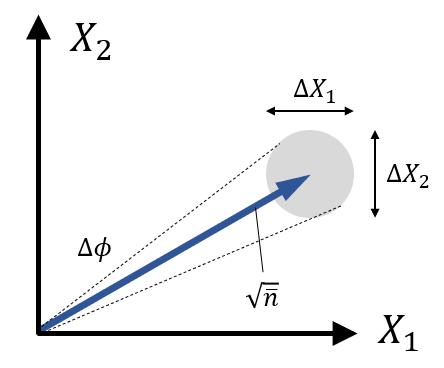
\includegraphics[width=0.4\linewidth]{quadrature.estados.coerentes.png}
    \caption{Quadrature representation of a coherent state. Number-phase uncertainty is represented by the gray circle.}
    \label{quadrature.coherent}
\end{figure}

In section \ref{considerações estatísticas}, we wrote a rigorous demonstration that:

\begin{equation}
    \Delta n = \sqrt{\bar{n}}
\end{equation}

But a more intuitive approach would be to say that, given that $\Delta X_1=\Delta X_2=1/2$:

\begin{equation}
    \Delta n = (\sqrt{\bar{n}}+1/4)^2-(\sqrt{\bar{n}}-1/4)^2=\sqrt{\bar{n}}
\end{equation}

It should be noted that $1/4$ is the \textbf{only} number for the uncertainty product that could generate this weird result: namely, that quadrature uncertainty in coherent states predicts Poissonian photon statistics. That realisation leads to the most important, and somewhat obvious, conclusion: that \textbf{shot noise originates from quantum uncertainty in light}. 

We can also write the phase uncertainty via geometrical considerations. In the classical limit, when $\abs{\alpha}\ll1$, the phase uncertainty will correspond to the following subtended angle:

\begin{equation}
    \Delta \phi = \frac{1/4 - (-1/4)}{\abs{\alpha}}=\frac{1/2}{\sqrt{\bar{n}}}
\end{equation}

When not in the ``classical limit'', this uncertainty should only become larger, therefore:

\begin{equation}
    \Delta \phi \ge \frac{1/2}{\sqrt{\bar{n}}}
\end{equation}

\begin{equation}
    \Delta \phi \Delta n \ge \frac{1/2}{\sqrt{\bar{n}}}\Delta n
\end{equation}

Since $\Delta n = \sqrt{\bar{n}}$

\begin{equation}
    \boxed{\Delta \phi \Delta n \ge \frac{1}{2}}
    \label{phase.number.uncertainty}
\end{equation}

\subsection{Squeezed States}

Figure \ref{quadrature.squeezed.states} and Equation \ref{phase.number.uncertainty} will clearly lead to an interesting conclusion: \textbf{amplitude-squeezed light has sub-Poissonian photon statistics.}

\begin{figure}[H]
    \centering
    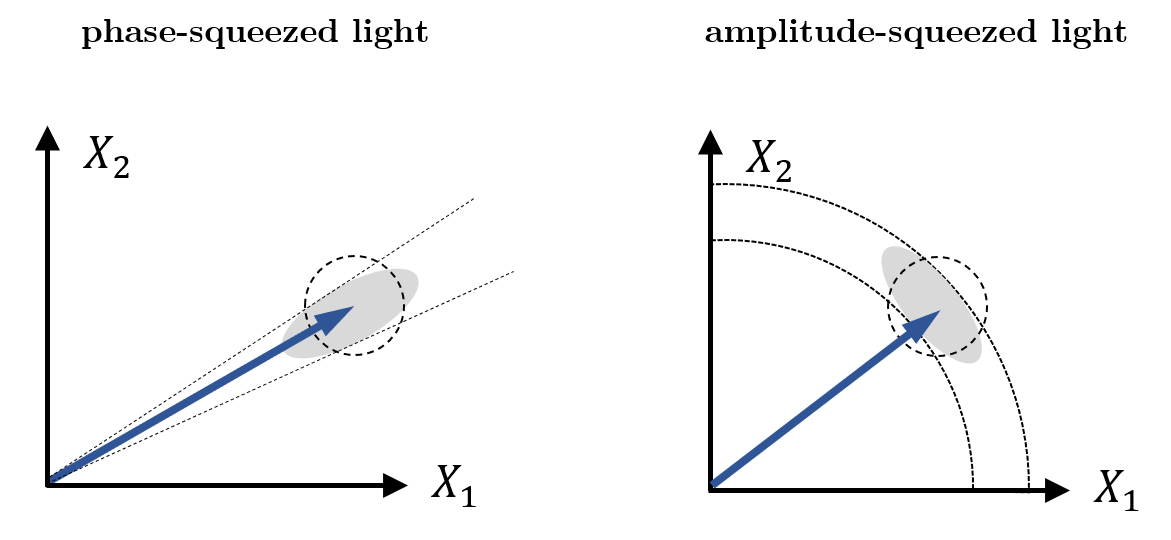
\includegraphics[width=1\linewidth]{quadrature.squeezed states.png}
    \caption{Quadrature-squeezed states. The shaded ellipse must have at least the same area as the circle.}
    \label{quadrature.squeezed.states}
\end{figure}

Accordingly, a photon number state has perfectly defined photon number $\Delta n =0$, and a completely undefined phase. Coherent states with $\Delta n =\sqrt{\bar{n}}$ have a much better defined phase.

\subsubsection{Detection of Squeezed Light}

Let us now consider the scheme in Figure \ref{balanced.homodyne.detecion}. If the experiment was made without any signal input, shot noise from the Poissonian statistics of the local oscillator will manifest itself in $i_1$ and $i_2$. Since shot noise power is proportional to the average photocurrent, its combined magnitude in both arms must be equal to that of the shot noise in the local oscillator. Additionally, since the noise is random, and therefore completely uncorrelated, shot noise in both currents will add at the output.


\begin{figure}[H]
    \centering
    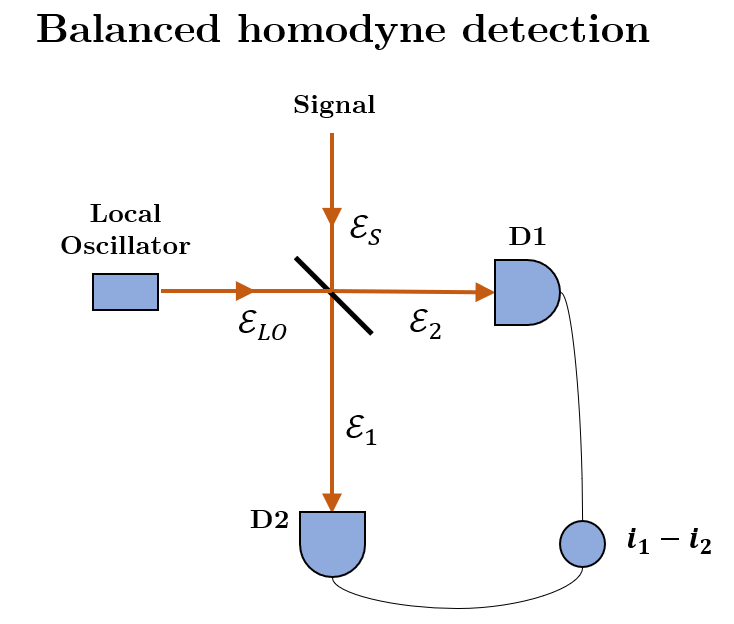
\includegraphics[width=0.6\linewidth]{balanced homodyne detection.png}
    \caption{Scheme for Balanced Homodyne Detection}
    \label{balanced.homodyne.detecion}
\end{figure}

Let us consider what happens if a signal is fed into the system.

\begin{equation}
    \mathcal{E}_1=\frac{1}{\sqrt{2}}\big(e^{i\phi_{LO}}\mathcal{E}_{LO}+\mathcal{E}_{s}\big)
\end{equation}

\begin{equation}
    \mathcal{E}_2=\frac{1}{\sqrt{2}}\big(e^{i\phi_{LO}}\mathcal{E}_{LO}-\mathcal{E}_{s}\big)
\end{equation}

Where the beam splitter has introduced a $\pi$ phase-shift for reflection. The local oscillator signal has large amplitude, and therefore can be treated classically. For the signal, however, we shall introduce a quadrature representation:

\begin{equation}
    \mathcal{E}_s=\mathcal{E}_S^{X_1}+i\mathcal{E}_S^{X_2}
\end{equation}

The $\pi/2$ phase-shift between the two quadratures is obvious from their definitions in Equation \ref{field.quad.amplitudes.equations}. It is now easy to see that:

\begin{equation}
    \mathcal{E}_1=\frac{1}{\sqrt{2}}\Big[   \big(\mathcal{E}_{LO}\cos(\phi_{LO})+\mathcal{E}_S^{X_1}\big)  +i\big(\mathcal{E}_{LO}\sin(\phi_{LO})+\mathcal{E}_S^{X_2}\big)\Big]
\end{equation}

\begin{equation}
    \mathcal{E}_2=\frac{1}{\sqrt{2}}\Big[   \big(\mathcal{E}_{LO}\cos(\phi_{LO})-\mathcal{E}_S^{X_1}\big)  +i\big(\mathcal{E}_{LO}\sin(\phi_{LO})-\mathcal{E}_S^{X_2}\big)\Big]
\end{equation}

The photocurrents generated in each detector are proportional to the input power, as we saw previously:

\begin{equation}
    i=\eta e \Phi=\eta e \frac{P}{\hbar\omega}
\end{equation}

Thus the measured output, which is given by the difference in the photocurrents:

\begin{equation}
    i_{out}\propto i_1-i_2
\end{equation}

Can be written in terms of the fields as follows:

\begin{equation}
    i_{out}\propto \mathcal{E}_1\mathcal{E}_1^*-\mathcal{E}_2\mathcal{E}_2^*
\end{equation}

\begin{multline}
    i_{out}\propto \abs{\frac{1}{\sqrt{2}}\Big[   \big(\mathcal{E}_{LO}\cos(\phi_{LO})+\mathcal{E}_S^{X_1}\big)  +i\big(\mathcal{E}_{LO}\sin(\phi_{LO})+\mathcal{E}_S^{X_2}\big)\Big]}^2+\\-\abs{\frac{1}{\sqrt{2}}\Big[   \big(\mathcal{E}_{LO}\cos(\phi_{LO})-\mathcal{E}_S^{X_1}\big)  +i\big(\mathcal{E}_{LO}\sin(\phi_{LO})-\mathcal{E}_S^{X_2}\big)\Big]}^2
\end{multline}

\begin{multline}
    2i_{out}\propto \big(\mathcal{E}_{LO}\cos(\phi_{LO})+\mathcal{E}_S^{X_1}\big)^2  +\big(\mathcal{E}_{LO}\sin(\phi_{LO})+\mathcal{E}_S^{X_2}\big)^2+\\-   \big(\mathcal{E}_{LO}\cos(\phi_{LO})-\mathcal{E}_S^{X_1}\big)^2  -\big(\mathcal{E}_{LO}\sin(\phi_{LO})-\mathcal{E}_S^{X_2}\big)^2
\end{multline}

\begin{equation}
    2i_{out}\propto4\mathcal{E}_{LO}\cos(\phi_{LO})\mathcal{E}_S^{X_1}+4\mathcal{E}_{LO}\sin(\phi_{LO})\mathcal{E}_S^{X_2}
\end{equation}

\begin{equation}
    i_{out}\propto2\mathcal{E}_{LO}\Big(\cos(\phi_{LO})\mathcal{E}_S^{X_1}+\sin(\phi_{LO})\mathcal{E}_S^{X_2}\Big)
\end{equation}

The output depends on the phase of the local oscillator. We can therefore explore the orthogonality of the quadratures in order to isolate their contributions to the output signal. \textbf{The balanced homodyne detector selects the signal field quadrature that is in phase with the local oscillator.}

We saw earlier that the absence of a signal input leads to shot noise in the output. In quantum optics, the null signal input is equivalent to vacuum modes entering the detector. Therefore the output measurement $\mathcal{E}_{LO}\mathcal{E}^{vac}$ has selected for the vacuum field, and in doing so, produced shot noise in the output. Stating this in yet another way, \textbf{the measurement of shot noise in the output can be treated as a consequence of homodyning the local oscillator with the vacuum field.}




















%\begin{equation*}
   % \mathcal{E}_x(z,t)=\big[\mathcal{E}_0\sin(kz)\cos(\%varphi)\big]\sin{\omega %t}+\big[\mathcal{E}_0\sin(kz)\sin(\varphi)\big]\cos%{\omega t}
%\end{equation*}
%
%The two amplitudes inside the square brackets are %called the \textbf{field quadratures}:
%
%\begin{equation}
%    \mathcal{E}_x(z,t)=\mathcal{E}_1\sin{\omega %t}+\mathcal{E}_2\cos{\omega t}
%\end{equation}
























































%===============================================================================================================================================================================================================================================================================================================================================================================================================================================================
\chapter{Notas: Vídeos Explicativos}

\section{Beam Splitter}\label{beam.splitter.section}

\subsection{O Problema}

O divisor de feixes é um dispositivo ótico que divide um feixe de luz em dois \cite{Loudon448s}. A Figura \ref{beam.splitter} mostra um esquema para um divisor ideal sem perdas.

\begin{figure}[H]
    \centering
    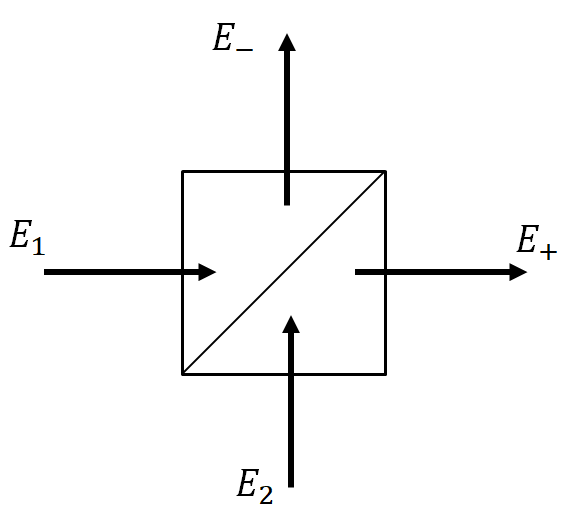
\includegraphics[width=0.3\linewidth]{beamsplitter.png}
    \caption{Divisor de Feixes}
    \label{beam.splitter}
\end{figure}

Queremos encontrar uma relação entre os campos de entrada $E_1$ e $E_2$ e os de saída $E_+$ e $E_{-}$, partindo de duas considerações iniciais:

\begin{enumerate}
    \item A linearidade do efeito do divisor sobre os feixes:
    \begin{equation}
        E_{\pm}=a_{\pm}E_1+b_{\pm}E_2
        \label{linearidade}
    \end{equation}
    \item A lei de conservação de energia
    \begin{equation}
        \abs{E_{+}}^2+\abs{E_{-}}^2=\abs{E_{1}}^2+\abs{E_{2}}^2
        \label{conservacao}
    \end{equation}
\end{enumerate}

Obs.: Todas as variávis são complexas.

\subsection{Módulo Quadrado |E|^2}

O primeiro passo é escrever o módulo quadrado de $E_{\pm}$ em função de $E_1$ e $E_2$:

\begin{equation}
    \abs{E_{\pm}}^2=\abs{a_{\pm}E_1+b_{\pm}E_2}^2
    \label{modulo.quadrado}
\end{equation}

Lembrando do seguinte resultado:
\begin{align*}
|z+w|^2 & = (z+w)(z^* + w^*)\\
        & = zz^*+zw^*+wz^*+ww^*\\
        & = \abs{z}^2+\abs{w}^2+(zw^*+wz^*)\\
\end{align*}

Se escrevermos $z=a_{\pm}E_1$ e $w=b_{\pm}E_2$, ficamos com:

\begin{equation*}
   \abs{a_{\pm}E_1+b_{\pm}E_2}^2 = \abs{a_{\pm}}^2\abs{E_{1}}^2+\abs{b_{\pm}}^2\abs{E_{2}}^2+a_{\pm}E_1(b^*_{\pm}E^*_2)+b_{\pm}E_2(a^*_{\pm}E^*_1)
\end{equation*}

Esses últimos dois termos podem ser reescritos usando:

\begin{equation*}
    a_{\pm}E_1(b^*_{\pm}E^*_2)+b_{\pm}E_2(a^*_{\pm}E^*_1)=2\Re(a_{\pm}E_1b^*_{\pm}E^*_2)
\end{equation*}

Cuja demonstração pode ser estendida facilmente a partir $z=(a+ib)$ e $w=(c+id)$:
\begin{align*}
zw^*+wz^*   & = (a+ib)(c-id)+(a-ib)(c+id)\\
            & = (ac-iad+ibc+bd)+(ac+iad-ibc+bd)\\
            & = (ac+bd+ad+bd)\\
            & = 2(ac+bd)\\
            & = 2\Re(zw^*)
\end{align*}

E então a Equação \ref{modulo.quadrado} fica:
\begin{equation}
   \boxed{\abs{E_{\pm}}^2=\abs{a_{\pm}}^2\abs{E_{1}}^2+\abs{b_{\pm}}^2\abs{E_{2}}^2+2\Re(a_{\pm}E_1b^*_{\pm}E^*_2)}
   \label{identity.sq.abs}
\end{equation}
Mas sabemos que:
\begin{equation}
    \Re(zw)=\Re(z)\Re(w)-\Im(z)\Im(w)
\end{equation}
Que é uma consequência evidente da seguinte identidade trigonométrica:
\begin{equation}
    \cos(a+b)=\cos(a)\cos(b)-\sin(a)\sin(b)
\end{equation}
Com essa identidade, chegamos na forma final da Equação \ref{modulo.quadrado}:
\begin{equation*}
   \boxed{\abs{E_{\pm}}^2=\abs{a_{\pm}}^2\abs{E_{1}}^2 + \abs{b_{\pm}}^2\abs{E_{2}}^2 + 2\Re(a_{\pm}b^*_{\pm})\Re(E_1E^*_{2})- 2\Im(a_{\pm}b^*_{\pm})\Im(E_1E^*_{2})}
\end{equation*}

\subsection{Aplicando a Conservação de Energia}

Substituindo o resultado anterior na Equação \ref{conservacao}, ficamos com:
\begin{multline*}
|E_{+}|^2+|E_{-}|^2 =(|a_{+}|^2+|a_{-}|^2)|E_{1}|^2 + (|b_{+}|^2+|b_{-}|^2)|E_{2}|^2 +\\ +2\Re(E_1E^*_{2})[\Re(a_{+}b^*_{+})+\Re(a_{-}b^*_{-})]+\\-2\Im(E_1E^*_{2})[\Im(a_{+}b^*_{+})+\Im(a_{-}b^*_{-})]
\end{multline*}

E então, ainda pela Equação \ref{conservacao}:
\begin{multline*}
|E_{1}|^2+|E_{2}|^2 =(|a_{+}|^2+|a_{-}|^2)|E_{1}|^2 + (|b_{+}|^2+|b_{-}|^2)|E_{2}|^2 +\\ +2\Re(E_1E^*_{2})[\Re(a_{+}b^*_{+})+\Re(a_{-}b^*_{-})]+\\-2\Im(E_1E^*_{2})[\Im(a_{+}b^*_{+})+\Im(a_{-}b^*_{-})]
\end{multline*}

Para que essa igualdade se mantenha para quaisquer dois campos $E_1$ e $E_2$ arbitrários, é preciso que:

\begin{equation*}
\begin{cases}
    |a_{+}|^2+|a_{-}|^2=1\\[0.3cm]
    |b_{+}|^2+|b_{-}|^2=1\\[0.3cm]
    \begin{cases}
        \Re(a_{+}b^*_{+})+\Re(a_{-}b^*_{-})=0\\
        \Im(a_{+}b^*_{+})+\Im(a_{-}b^*_{-})=0\\
    \end{cases}
\end{cases}
\end{equation*}

Esses conjunto de condições pode ser simplificado para:

\begin{equation}
\begin{cases}
    |a_{+}|^2+|a_{-}|^2=1\\[0.3cm]
    |b_{+}|^2+|b_{-}|^2=1\\[0.3cm]
    a_+b^*_{+}+a_{-}b^*_{-}=0
\end{cases}
\label{sistema}
\end{equation}

\subsection{Resolvendo o Sistema}

Escrevendo as constantes $a_{\pm}$ e $b_{\pm}$ em notação complexa polar:

\begin{equation}
\begin{cases}
    a_{\pm} = |a_{\pm}|\exp(i\alpha_{\pm})\\[0.3cm]
    b_{\pm} = |b_{\pm}|\exp(i\beta_{\pm})\\
\end{cases}
\end{equation}

Substituindo na terceira equação de \ref{sistema}, ficamos com:

\begin{equation*}
    |a_{+}|\exp(i\alpha_{+})|b_{+}|\exp(-i\beta_{+})+|a_{-}|\exp(i\alpha_{-})|b_{-}|\exp(-i\beta_{-})=0
\end{equation*}

\begin{equation*}
    |a_{+}||b_{+}|\exp(i\alpha_{+}-i\beta_{+})+|a_{-}||b_{-}|\exp(i\alpha_{-}-i\beta_{-})=0
\end{equation*}

A equação acima leva imediatamente a:

\begin{equation}
\begin{cases}
    \exp{i(\alpha_{+}-\beta_{+})} = -\exp{i(\alpha_{-}-\beta_{-})}\\[0.3cm]
    |a_{+}||b_{+}|=|a_{-}||b_{-}|
\end{cases}
\end{equation}

A primeira equação do sistema claramente descreve dois números complexos ao longo do circulo unitário, defasados por $\pi$:

\begin{equation}
    \boxed{\alpha_{+}-\beta_{+}=\alpha_{-}-\beta_{-}+\pi}
    \label{phase.shift}
\end{equation}

E então restam apenas as equações referentes a $a_{\pm}$ e $b_{\pm}$, que formam um sistema não-linear:

\begin{equation}
\begin{cases}
    |a_{+}|^2+|a_{-}|^2=1\\[0.3cm]
    |b_{+}|^2+|b_{-}|^2=1\\[0.3cm]
    |a_{+}||b_{+}|=|a_{-}||b_{-}|
\end{cases}
\end{equation}\\

Elevando a terceira equação ao quadrado:

\begin{equation}
\begin{cases}
    |a_{+}|^2+|a_{-}|^2=1\\[0.3cm]
    |b_{+}|^2+|b_{-}|^2=1\\[0.3cm]
    |a_{+}|^2|b_{+}|^2=|a_{-}|^2|b_{-}|^2
\end{cases}
\label{coeficientes}
\end{equation}

Substituindo a primeira e a segunda na terceira:

\begin{equation}
    |a_{+}|^2(1-|b_{-}|^2)=(1-|a_{+}|^2)|b_{-}|^2
\end{equation}

\begin{equation}
    |a_{+}|^2-|a_{+}|^2|b_{-}|^2=|b_{-}|^2-|a_{+}|^2|b_{-}|^2
\end{equation}

Somando $|a_{+}|^2|b_{-}|^2$ nos dois lados, ficamos com:

\begin{equation}
    |a_{+}|^2=|b_{-}|^2 \Rightarrow |a_{+}|=|b_{-}|
\end{equation}

Fazendo um procedimento perfeitamente análogo para as outras duas variáveis, ficamos com:

\begin{equation}
\begin{cases}
    |a_{+}|=|b_{-}|\\[0.3cm]
    |a_{-}|=|b_{+}|
\end{cases}
\end{equation}

\subsection{Significado Físico dos Parâmetros}

Podemos resumir os resultados das últimas seções na seguinte imagem:

\begin{figure}[H]
    \centering
    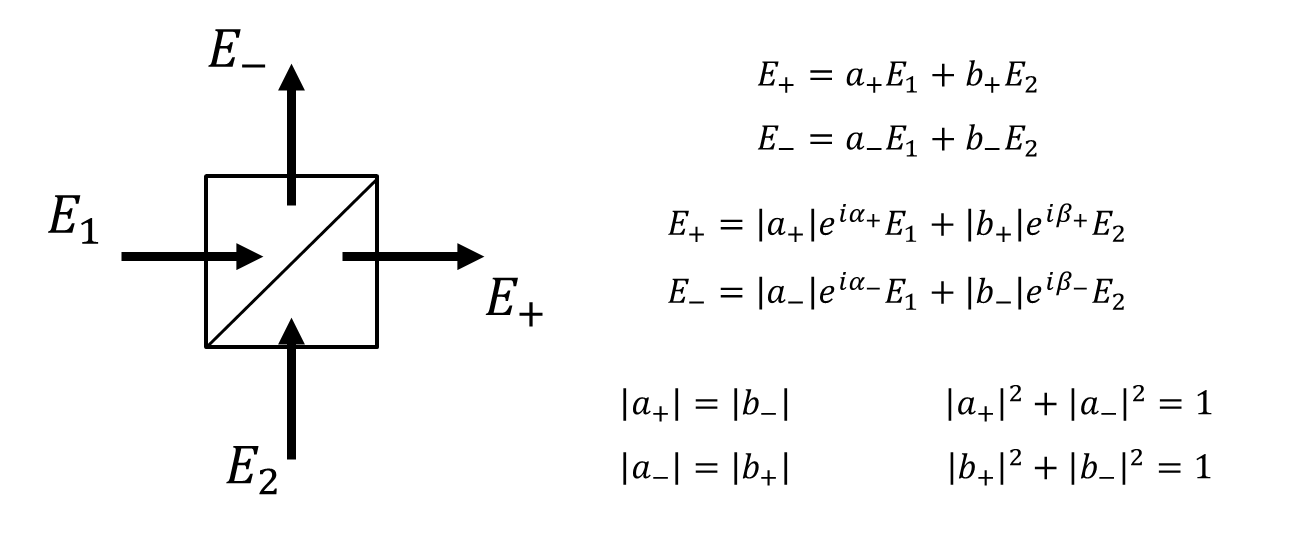
\includegraphics[width=0.9\linewidth]{results.png}
    \caption{Resumo dos Resultados Anteriores}
    \label{resumo}
\end{figure}

Aqui fica evidente que:

\begin{itemize}
    \item $|a_+|$ media a relação de $E_1$ com o feixe $E_+$, que preserva sua direção.
    \item $|b_-|$ media a relação de $E_2$ com o feixe $E_-$, que preserva sua direção.
    \item $|a_-|$ media a relação de $E_1$ com o feixe $E_-$, que troca sua direção.
    \item $|b_+|$ media a relação de $E_1$ com o feixe $E_+$, que troca sua direção.
\end{itemize}

Portanto é natural tomar $|a_+|$ e $|b_-|$ como parâmetros associados a transmissão, e $|a_-|$ e $|b_+|$ como parâmetros associados a reflexão.\\

Das relações compiladas na Figura \ref{resumo}, é intuitivo sugerir que:

\begin{equation*}
    \begin{cases}
        |a_+|=|b_-|=\sqrt{T}\\
        |a_-|=|b_+|=\sqrt{R}
    \end{cases}
\end{equation*}

Portanto, pelas duas primeiras equações em \ref{coeficientes}, obtemos que:

\begin{equation}
    \boxed{T+R=1}
\end{equation}

Como consequência necessária da lei de conservação da energia.\\

Reescrevendo os campos de saída $E_+$ e $E_-$ a partir das novas definições:

\begin{equation}
    \begin{cases}
        E_+=\sqrt{T}e^{i\alpha_+}E_1+\sqrt{R}e^{i\beta_+}E_2\\
        E_-=\sqrt{R}e^{i\alpha_-}E_1+\sqrt{T}e^{i\beta_-
        }E_2
    \end{cases}
    \label{campos}
\end{equation}

\subsection{Mudança de Variáveis e Fase Global}

Queremos introduzir uma mudança de variáveis que implique em:

\begin{itemize}
    \item Uma fase global
    \item Simetria entre as expressões para os campos
\end{itemize}

A partir das Equações em \ref{campos}, podemos escrever:

\begin{equation}
    \begin{cases}
        E_+=\sqrt{T}\exp(i\alpha_+)E_1+\sqrt{R}\exp(i\beta_+)E_2\\
        E_-=\sqrt{R}\exp(i\alpha_-)E_1+\sqrt{T}\exp(i\beta_-)E_2
    \end{cases}
    \label{campos}
\end{equation}

Vamos introduzir as seguintes mudanças. A motivação para as escolhas ficará clara diante dos resultados:

\begin{equation}
    \begin{cases}
        \theta=\frac{(\alpha_++\beta_-)}{2}\\[0.3cm]
        \varphi=\alpha_+-\beta_-\\
        \Delta=\alpha_+-\beta_+
    \end{cases}
    \label{mudancas}
\end{equation}

Precisamos escrever $\alpha_+$, $\beta_+$, $\alpha_-$, $\beta_-$ em função dessas variáveis:

\begin{align*}
\alpha_+     & = \theta+\frac{\varphi}{2}\\[0.3cm]
\beta_+      & = \theta+\frac{\varphi}{2}-\Delta\\[0.3cm]
\alpha_-     & = (\theta-\frac{\varphi}{2}+\Delta)+\pi\\[0.3cm]
\beta_-      & = \theta-\frac{\varphi}{2}\\
\end{align*}

Todas as expressão são facilmente verificadas por substituição direta em \ref{mudancas}. A exceção é $\alpha_-$, que demonstramos a seguir:

\begin{align*}
\theta-\frac{\varphi}{2}+\Delta & =[(\frac{(\alpha_++\beta_-)}{2})]-[\frac{\alpha_+-\beta_-}{2}]+[\alpha_+-\beta_+]\\
            & = \frac{\alpha_++\beta_--\alpha_++\beta_-+2\alpha_+-2\beta_+}{2}\\
            & = \beta_-+[\alpha_+-\beta_+]\\
            & = \beta_-+[\alpha_--\beta_-+\pi]\\
            & = \alpha_-+\pi\\
\end{align*}

Onde usamos a Equação \ref{phase.shift}, que dá $\alpha_+-\beta_+=\alpha_--\beta_-+\pi$.\\

Pela identidade de Euler, $\pi$ introduz um sinal na equação. E com essas substituições a Equação \ref{campos} fica:

\begin{equation}
    \begin{cases}
        E_+=\exp(i\theta)[\sqrt{T}\exp(i\frac{\varphi}{2})E_1+\sqrt{R}\exp(i(\frac{\varphi}{2}-\Delta))E_2] \\[0.3cm]
        E_-=\exp(i\theta)[-\sqrt{R}\exp(-i(\frac{\varphi}{2}-\Delta))E_1+\sqrt{T}\exp(-i\frac{\varphi}{2})E_2]
    \end{cases}
\end{equation}

Reorganizando:

\begin{equation}
    \begin{cases}
        E_+=\exp(i\theta)[\sqrt{T}\exp(i\frac{\varphi}{2})E_1+\sqrt{R}\exp(i(\frac{\varphi}{2}-\Delta))E_2] \\[0.3cm]
        E_-=\exp(i\theta)[\sqrt{T}\exp(-i\frac{\varphi}{2})E_2-\sqrt{R}\exp(-i(\frac{\varphi}{2}-\Delta))E_1]
    \end{cases}
    \label{campos.novo}
\end{equation}

Aqui fica claro que os objetivos mencionados no começo da sessão foram atingidos:

\begin{itemize}
    \item O termo $e^{i\theta}$ introduz uma fase global que podemos definir como $\theta=0$ \textbf{sem qualquer perda de generalidade}
    \item As demais fases apresentam forte simetria
\end{itemize}

Com a definição de $\theta=0$, ficamos com:

\begin{align*}
\alpha_+     & = \theta+\frac{\varphi}{2} \Rightarrow \frac{\varphi}{2}\\[0.3cm]
\beta_+      & = \theta+\frac{\varphi}{2}-\Delta \Rightarrow \frac{\varphi}{2}-\Delta\\[0.3cm]
\alpha_-     & = (\theta-\frac{\varphi}{2}+\Delta)+\pi \Rightarrow -(\frac{\varphi}{2}-\Delta)+\pi\\[0.3cm]
\beta_-      & = \theta-\frac{\varphi}{2} \Rightarrow -\frac{\varphi}{2}\\
\end{align*}

Com efeito, agora podemos definir dois parâmetros:

\begin{equation*}
t=\sqrt{T}\exp(i\frac{\varphi}{2})=\sqrt{T}\exp(i\alpha_+)
\end{equation*}

\begin{equation*}
r=\sqrt{R}\exp(i(\frac{\varphi}{2}-\Delta))=\sqrt{R}\exp(i\beta_+)
\end{equation*}

E então, com essas definições de $r$ e $t$, as equações dos campos se tornam:

\begin{equation*}
    \boxed{E_+=t E_1+r E_2}
\end{equation*}

\begin{equation*}
    \boxed{E_-=-r^*E_1+t^*E_2}
\end{equation*}

Finalmente, podemos escrever uma equação matricial:

\begin{equation*}
    \begin{pmatrix}E_+\\E_-\end{pmatrix}=\begin{pmatrix}t & r\\-r^* & t^*\end{pmatrix} \begin{pmatrix}E_1\\E_2\end{pmatrix}
\end{equation*}

que descreve o divisor de feixes ideal.

\begin{figure}[H]
    \centering
    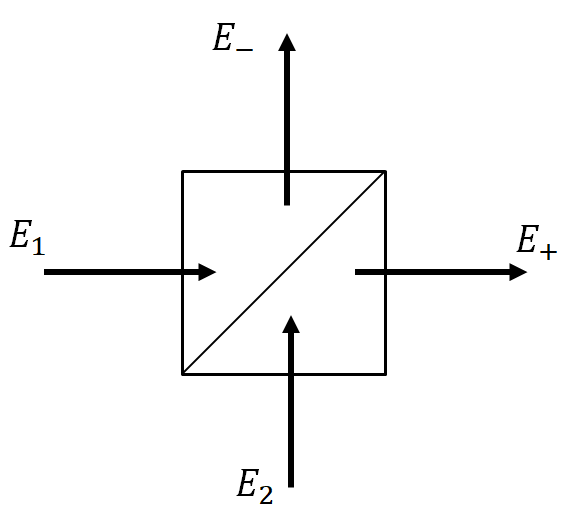
\includegraphics[width=0.3\linewidth]{beamsplitter.png}
    \caption{Divisor de Feixes}
    \label{beam.splitter}
\end{figure}
\pagebreak
\section{Estados Coerentes}\label{estados.coerentes.section}

\subsection{Revisão: Oscilador Harmônico Quântico}\label{quantum.harmonic.oscillator}

Suponha um sistema cuja Hamiltoniana é:

\begin{equation}
    H=\frac{p^2}{2m}+\frac{m\omega^2x^2}{2}
\end{equation}

Vamos definir os seguintes operadores de aniquilação a criação:

\begin{equation}
    \begin{cases}
        a=\sqrt{\frac{m\omega}{2\hbar}}(x+\frac{ip}{m\omega}) \\[0.3cm]
        a^{\dag}=\sqrt{\frac{m\omega}{2\hbar}}(x-\frac{ip}{m\omega})
    \end{cases}
\end{equation}

Tais que $\comm{a}{a^{\dag}}=1$. Fácil de verificar usando $\comm{x_i}{F(\textbf{p})}=i\hbar\frac{\partial{F}}{\partial{p_i}}$. A partir desses, definimos o operador número:

\begin{equation}
    N=a^{\dag}a
\end{equation}

\begin{equation}
    \therefore N=\frac{H}{\hbar\omega}-\frac{1}{2}
    \label{NeH}
\end{equation}

Isso implica que podemos diagonalizar H e N simultaneamente para obter uma base de autokets de energia que também são autokets de N.\\

A partir da Equação \ref{NeH} é fácil ver que:

\begin{equation*}
    N\ket{n}=n\ket{n} \Rightarrow H\ket{n}=(n+\frac{1}{2})\hbar\omega\ket{n}
\end{equation*}

A motivação para as definições de $a$ e $a^{\dag}$ ficam claras quando consideramos seu comportamento enquanto:

\begin{itemize}
    \item Autokets do operador N:
    \begin{equation*}
        \begin{cases}
            Na^{\dag}\ket{n}=(n+1)a^{\dag}\ket{n}\\
            Na\ket{n}=(n-1)a\ket{n}
        \end{cases}
    \end{equation*}
    \item Autokets de $\ket{n}$:
    \begin{equation*}
        \begin{cases}
            a^{\dag}\ket{n}=\sqrt{n+1}\ket{n+1}\\
            a\ket{n}=\sqrt{n}\ket{n-1}
        \end{cases}
        \label{efeito.cria.anaq}
    \end{equation*}
\end{itemize}

Para que uma sequência de aplicações do operador de destruição seja interrompida em $\ket{0}$, é preciso que $n$ seja um inteiro positivo. Isso permite definir a energia do estado fundamental:

\begin{equation*}
    \ket{0}=\frac{1}{2}\hbar\omega
\end{equation*}

E a partir dela a expressão de um ket $\ket{n}$ qualquer:

\begin{equation}
    \boxed{\ket{n}={\frac{(a^{\dag})^n}{\sqrt{n!}}}\ket{0}}
\end{equation}

Usando apenas a discussão acima, é possível todas as demais relações de comutação, elementos de matrizes e representação em coordenadas. Destaco aqui os resultados mais importantes:

\begin{equation*}
    x=\sqrt{\frac{\hbar}{2m\omega}}(a+a^{\dag})
\end{equation*}

\begin{equation*}
    p=i\sqrt{\frac{m\hbar\omega}{2}}(-a+a^{\dag})
\end{equation*}

\begin{equation}
    \braket{x}{0}=\frac{1}{\pi^{1/4}\sqrt{x_0}}\exp(-\frac{1}{2}\frac{x^2}{x^2_0})
\end{equation}

A aplicação da equação de movimento de Heisenberg leva facilmente à seguinte solução para a evolução temporal de $x(t)$ e $p(t)$:

\begin{equation}
    x(t)=x(0)\cos(\omega t)+\frac{p(0)}{m\omega}\sin(\omega t)    
\end{equation}

\begin{equation}
    p(t)=-m\omegax(0)\sin(\omega t)+p(0)\cos(\omega t)    
\end{equation}

\subsection{Escrevendo um Estado Coerente na Base de Fock}

Dado um estado coerente, auto-estado do operador de aniquilação:

\begin{equation}
    \ket{\alpha} \Rightarrow a\ket{\alpha}=\alpha\ket{\alpha}
    \label{definicao.coerente}
\end{equation}

Queremos representar $\ket{\alpha}$ na base de Fock (autokets do operador N). Naturalmente:

\begin{equation}
    \ket{\alpha}=\sum_{n=0}^{\infty}c_n\ket{n}
\end{equation}

E o objetivo é encontrar os coeficientes:

\begin{equation}
        \braket{n'}{\alpha}=\sum_{n=0}^{\infty}c_n\braket{n'}{n}\therefore \braket{n'}{\alpha}=\sum_{n=0}^{\infty}c_n\delta_{nn'}  \therefore  c_n=\braket{n}{\alpha}
        \label{definicao.coeficiente}
\end{equation}

Agora vamos operar sobre o ket $\alpha$:
\begin{equation*}
    \bra{n-1}a\ket{\alpha}=(a^{\dag}\ket{n-1})^{\dag}\ket{\alpha}=(\sqrt{n}\ket{n})^{\dag}\ket{\alpha}=\sqrt{n}\braket{n}{\alpha}=\sqrt{n}c_n
\end{equation*}
\begin{equation}
    \therefore\bra{n-1}a\ket{\alpha}=\sqrt{n}c_n
\end{equation}

E usando também as Equações \ref{definicao.coerente} e \ref{definicao.coeficiente}, podemos escrever:

\begin{equation*}
    \bra{n-1}a\ket{\alpha}=\alpha\braket{n-1}{\alpha}=\alpha c_{n-1}
\end{equation*}

Isso dá origem a uma relação de recorrência:

\begin{equation}
    \sqrt{n}c_n=\alpha c_{n-1}
\end{equation}

Prolongado a relação até o estado fundamental \ket{0}:

\begin{equation}
    c_n=\frac{\alpha^n}{\sqrt{n!}}c_0
\end{equation}

Então nossa equação inicial vira:

\begin{equation}
   \boxed{\ket{\alpha}=c_0\sum_{n=0}^{\infty}\frac{\alpha^n}{\sqrt{n!}}\ket{n}}
\end{equation}

\subsection{Encontrando a Constante de Normalização}

Exigindo $\braket{\alpha}=1, \forall\ket{\alpha}$:

\begin{equation}
    \braket{\alpha}=\abs{c_0}^2\sum_{n=0}^{\infty}\frac{\alpha^n}{\sqrt{n!}}\sum_{m=0}^{\infty}\frac{(\alpha^*)^n}{\sqrt{m!}}\braket{m}{n}
\end{equation}

Usando $\braket{m}{n}=\delta_{mn}$

\begin{equation}
    \braket{\alpha}=\abs{c_0}^2\sum_{n=0}^{\infty}\frac{\abs{\alpha}^{2n}}{n!}
\end{equation}

Ou seja:

\begin{equation}
    \braket{\alpha}=\abs{c_0}^2\exp(\abs{\alpha}^2)
\end{equation}

Para obter $\braket{\alpha}=1$, é natural definir:

\begin{equation}
    \abs{c_0}=\exp(-\frac{\abs{\alpha}^2}{2})
\end{equation}

A condição de normalização não determina totalmente o coeficiente $c_0$. Podemos assumir que sua fase é nula ($c_0$ real) sem perda de generalidade.\\

Finalmente, a expressão para o estado coerente na base de Fock é:

\begin{equation}
   \boxed{\ket{\alpha}=e^{-\frac{\abs{\alpha}^2}{2}}\sum_{n=0}^{\infty}\frac{\alpha^n}{\sqrt{n!}}\ket{n}}
    \label{estado coerente na base de fock}
\end{equation} 

\subsection{Considerações Estatísticas}\label{considerações estatísticas}

O valor esperado do observável N em relação ao estado $\ket{n}$

\begin{equation*}
    \bra{n}N\ket{n}=\bra{n}a^{\dag}a\ket{n}=(a\ket{n})^{\dag}a\ket{n}=n\braket{n-1}{n-1}=n
\end{equation*}

Ou, ainda mais simples:

\begin{equation}
    \bra{n}N\ket{n}=\bra{n}n\ket{n}=n\braket{n}{n}=n
    \label{valor esperado N em n}
\end{equation}

Agora o valor esperado do observável N em relação a um estado coerente:

\begin{equation*}
    \langle N \rangle_\alpha=\bra{\alpha}N\ket{\alpha}=\bra{\alpha}a^{\dag}a\ket{\alpha}=a^*a\braket{\alpha}{\alpha}=\abs{\alpha}^2
\end{equation*}

Ou seja:

\begin{equation}
    \boxed{\langle N \rangle_\alpha=\abs{\alpha}^2}
    \label{valor esperado N em alpha}
\end{equation}

A partir daí podemos definir a dispersão $\langle(\Delta A)^2\rangle$ e o desvio padrão $\sigma(A)$, sabendo que:

\begin{equation}
    \sigma(A)=\sqrt{\langle(\Delta A)^2\rangle}=\sqrt{\langle A^2\rangle-\langle A \rangle^2}
\end{equation}

Pela Equação \ref{valor esperado N em n} é fácil ver que:

\begin{equation}
    \langle(\Delta N)^2\rangle_n=0
\end{equation}

Já a dispersão para o operador N em relação ao estado coerente:

\begin{equation*}
    \langle(\Delta N)^2\rangle_\alpha=\bra{\alpha}a^{\dag}aa^{\dag}a\ket{\alpha}-\bra{\alpha}a^{\dag}a\ket{\alpha}
\end{equation*}
\begin{equation*}
    \langle(\Delta N)^2\rangle_\alpha=\bra{\alpha}a^{\dag}aa^{\dag}a\ket{\alpha}-\abs{\alpha}^2
\end{equation*}

E usando o comutador para os operadores de aniquilação e criação $\comm{a}{a^{\dag}}=1$:

\begin{equation*}
    \bra{\alpha}a^{\dag}aa^{\dag}a\ket{\alpha}=\bra{\alpha}a^{\dag}(a^{\dag}a+1)a\ket{\alpha}=\abs{\alpha}^2\bra{\alpha}(a^{\dag}a+1)\ket{\alpha}=\abs{\alpha}^2(\abs{\alpha}^2+1)
\end{equation*}

Ou seja:

\begin{equation*}
    \langle(\Delta N)^2\rangle_\alpha=\abs{\alpha}^2(\abs{\alpha}^2+1)-\abs{\alpha}^2
\end{equation*}

\begin{equation*}
    \langle(\Delta N)^2\rangle_\alpha=\abs{\alpha}^4
\end{equation*}

E o desvio padrão é:

\begin{equation}
    \boxed{\sigma(N)=\abs{\alpha}^2}
\end{equation}

Que é idêntico ao valor esperado $\langle N \rangle_\alpha$ encontrando na Equação \ref{valor esperado N em alpha}. \textbf{Portanto o valor esperado e o desvio padrão do observável ``número de fótons'' em relação a um estado coerente são iguais}.

\subsubsection{Estado Coerente como Distribuição de Poisson}

Qual a probabilidade de encontrar um estado coerente $\ket{\alpha}$ em $\ket{n}$? Vamos recorrer à Equação \ref{estado coerente na base de fock} para escrever:

\begin{equation*}
    \abs{\braket{n}{\alpha}}^2=\abs{c_n}^2=e^{-\abs{\alpha}^2}\frac{\abs{\alpha}^{2n}}{n!} 
\end{equation*}

E com os resultados que obtivemos na seção \ref{considerações estatísticas}:

\begin{equation*}
     \abs{\braket{n}{\alpha}}^2=e^{-\langle N \rangle}\frac{\langle N \rangle^n}{n!} 
\end{equation*}

A forma da equação acima é familiar: descreve uma distribuição de Poisson.

\begin{figure}[H]
    \centering
    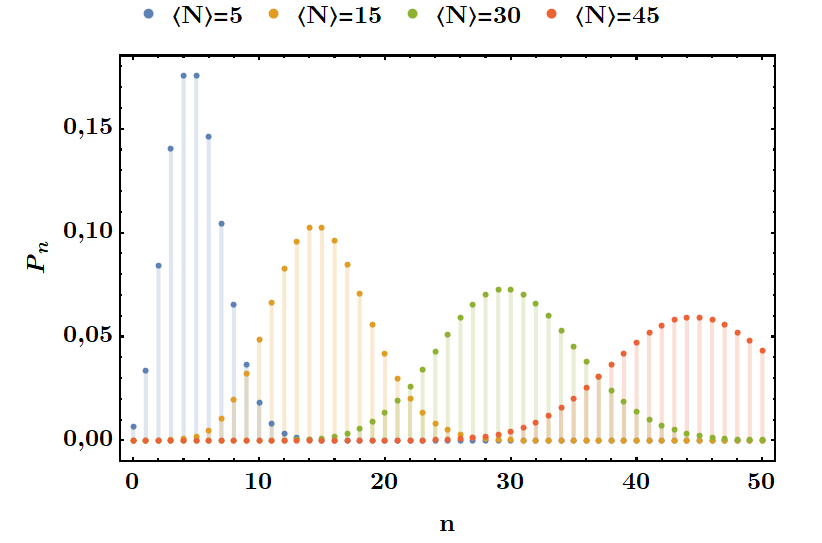
\includegraphics[width=0.7\linewidth]{Poisson.png}
    \caption{A probabilidade de medir um número \textit{n} de fótons segue uma distribuição de Poisson.}
    \label{Poisson}
\end{figure}

\subsection{Operador Deslocamento}

Retomando a expressão para o estado coerente na base de Fock:

\begin{equation}
   \ket{\alpha}=e^{-\frac{\abs{\alpha}^2}{2}}\sum_{n=0}^{\infty}\frac{\alpha^n}{\sqrt{n!}}\ket{n}
\end{equation}

Mas vimos na revisão do oscilador harmônico quântico que:

\begin{equation}
    \ket{n}={\frac{(a^{\dag})^n}{\sqrt{n!}}}\ket{0}
\end{equation}

Aplicando a última equação na primeira:

\begin{equation}
   \ket{\alpha}=e^{-\frac{\abs{\alpha}^2}{2}}\sum_{n=0}^{\infty}\frac{(a^{\dag}\alpha)^n}{n!}\ket{0}
\end{equation}

Que é uma série de potências para a seguinte exponencial:

\begin{equation}
   \ket{\alpha}=\exp\Bigr(-\frac{\abs{\alpha}^2}{2}\Bigl)\exp\Bigl(a^{\dag}\alpha\Bigr)\ket{0}
   \label{operador.criador.coerente}
\end{equation}

O fator do lado esquerdo da equação descreve um operador que cria um estado coerente a partir do estado de vácuo.

É fácil verificar que esse operador não satisfaz a definação de unitariedade:

\begin{equation*}
    U^{\dag}=U^{-1} q
\end{equation*}

Com efeito:

\begin{equation*}
    \Bigg[\exp\Bigr(-\frac{\abs{\alpha}^2}{2}\Bigl)\exp\Bigl(a^{\dag}\alpha\Bigr)\Bigg]^{\dag}=\Bigg[\exp\Bigr(-\frac{\abs{\alpha}^2}{2}\Bigl)\exp\Bigl(a\alpha^*\Bigr)\Bigg]\neq\Bigg[\exp\Bigr(-\frac{\abs{\alpha}^2}{2}\Bigl)\exp\Bigl(a^{\dag}\alpha\Bigr)\Bigg]^{-1}
\end{equation*}

Olhando para o segundo termo da equação acima, note que $\exp\Bigl(a\alpha^*\Bigr)$ não tem qualquer efeito ao ser aplicado sobre o estado de vácuo. Expandindo-o em uma série de potências, todos os termos que contém o operador de aniquilação serão nulos, e só restará a unidade.

Então vamos reescrever a Equação \ref{operador.criador.coerente} a partir dessa nova informação:

\begin{equation}
   \ket{\alpha}=\exp\Bigr(-\frac{\abs{\alpha}^2}{2}\Bigl)\exp\Bigl(a^{\dag}\alpha\Bigr)\exp\Bigl(-a\alpha^*\Bigr)\ket{0}
\end{equation}

Acrescentamos um sinal negativo no expoente. E agora definiremos esse fator como o \textbf{operador de deslocamento} (que cria um estado coerente a partir do estado de vácuo):

\begin{equation}
    D(\alpha)=\exp\Bigr(-\frac{\abs{\alpha}^2}{2}\Bigl)\exp\Bigl(a^{\dag}\alpha\Bigr)\exp\Bigl(-a\alpha^*\Bigr)
\end{equation}


















\pagebreak

\section{Interferômetro de Mach-Zehnder}\label{mach.zender.section}






\pagebreak











%===============================================================================================================================================================================================================================================================================================================================================================================================================================================================
\chapter{Course Notes: Micro and Nanofabrication}

\section{MEMS and Cleanroom Introduction}

\subsection{Case Study: Micro-Actuator}

As a first example of micro and nanofabrication, let us go through the process for making a \textbf{micro-actuator}.

An actuator is a component responsible for movements in a machine (such as opening a valve or flipping a switch). Here, we will deal with a thermo-mechanical micro-actuator, wich takes advantage of the difference in thermal expansion coefficients of two materials.

\begin{figure}[H]
    \centering
    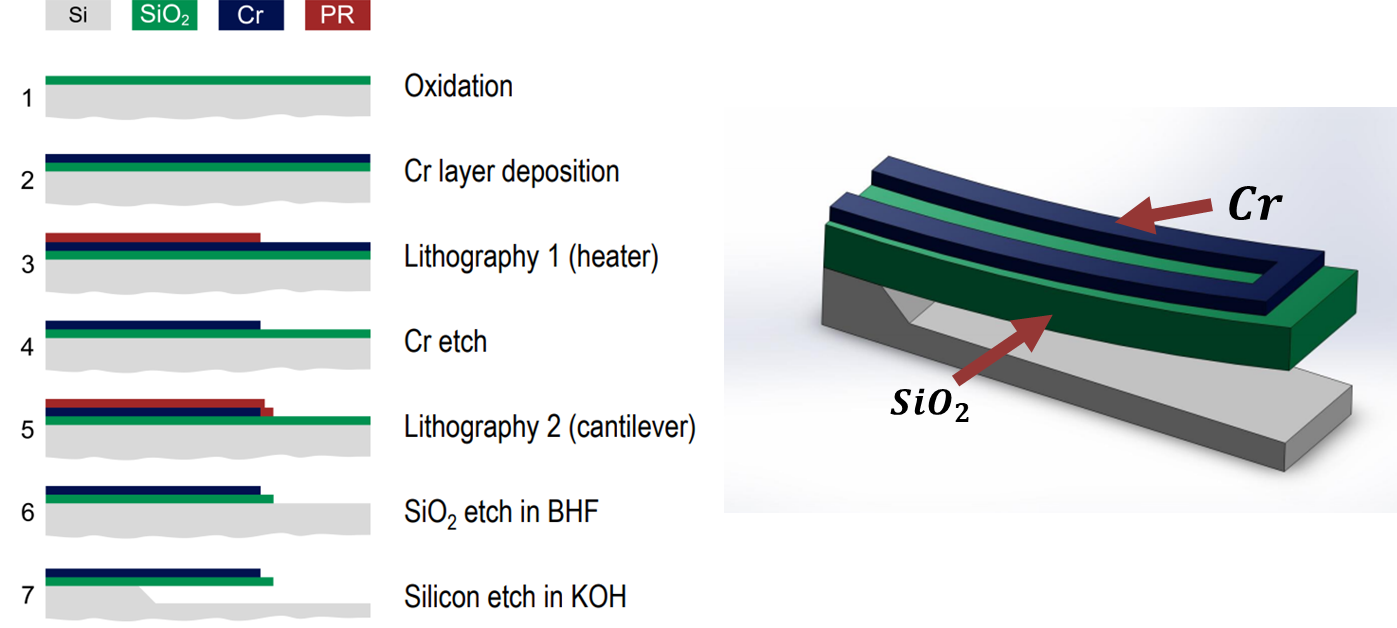
\includegraphics[width=1\linewidth]{micro actuator.png}
    \caption{Silicon Oxide and Chromium have different thermal expansion coefficients. When a voltage is applied to the chromium layer, a current will cause the system to heat up and dilation will occur. Difference in thermal coefficients will lead to controllable curvature radius.}
    \label{micro actuator procedure}
\end{figure}

Let us now go through the process of fabricating such a device.

\subsubsection{\#1: Wafer Preparation and Wet Oxidation}

A standard cleaning procedure is applied to the wafer, called RCA cleaning (\textit{Radio Corporation of America}):

\begin{enumerate}
    \item A solution of deionized water, ammonia water and hydrogen peroxide is applied at around $70\degree C$ for about 10 minutes \textbf{in order to remove organic residues.}
    \item The wafer is immersed in an acquose solution of hydrofluoric acid (HF) for about fifteen seconds at room temperature, \textbf{in order to remove the thin Silicon Dioxide layer that will be formed after step (1).}
    \item A solution of deionized water, hydrochloric acid and hydrogen peroxide is applied in the same conditions as step (1), \textbf{in order to remove remaining traces of metallic contaminants.}
    \item Rinsing and drying (air pistol).
\end{enumerate}

The wafers will then undergo \textbf{wet oxidation}, which is a form of hydro-thermal treatment. In this case, it should create a thin layer of \textbf{silicon oxide} whose \textbf{thickness can be controlled by adjusting temperature and exposure time}. For example, wet oxidation of an average sized silicon wafer at $1100\degree C$ for six hours will lead to a $1.5\mu m$ thick layer.

\subsubsection{\#2: Chromium Deposition by PVD}

A $500 nm$ layer of chromium is deposited using Electron-beam physical vapor deposition. This process will be discussed in greater detail later. Essentially, however, it consists of a controlled bombardment of a target anode with an electron beam given off by a tungsten filament under high vacuum. The target material will than transform into the gas phase and precipitate into a coating upon the wafer.

So now we are left with a silicon wafer coated with two layers: the first is wet-oxidation-grown silicon oxide, and the second is e-beam PVD-deposited chromium.

\subsubsection{\#3: Photolitography to Pattern the Chromium Heaters}

Photolitography is an essential step of almost any microfabrication process. A more detailed discussion will follow below. But a standard procedure consists of the following steps:

\begin{enumerate}
    \item Application and spinning of adhesion promoter (HMDS);
    \item Application and spinning of photoresists coating;
    \item Soft-baking at around $90\degree C$;
    \item Exposure to UV light under the appropriate pattern-printing mask;
    \item Development in order to remove/preserve the exposed parts of photoresist coating;
\end{enumerate}

\subsubsection{\#4 Chromium Etching}

Once the photoresist has been patterned, we may now proceed to etching the chrome. In this particular case, it can be done through immersion into a chromate solution. Afterwards, the photoresists is removed and the wafer is cleaned once again.

\subsubsection{\#5 Second Litography and Oxide Etching}

A similar set of procedures is then repeated in order to etch the silicon oxide layer and the silicon substrate as shown in steps (5)-(6) in Figure \ref{micro actuator procedure}.

\begin{figure}[H]
    \centering
    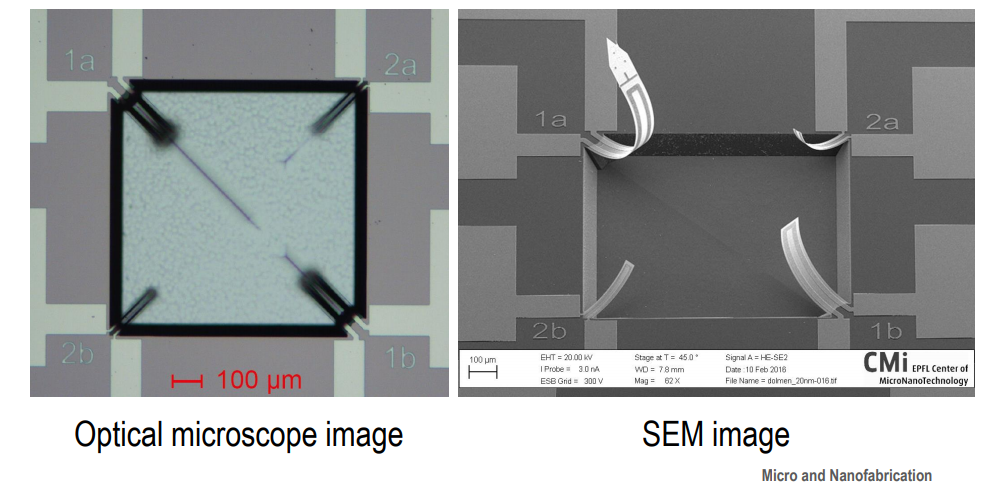
\includegraphics[width=0.8\linewidth]{final micro-actuator.png}
    \caption{Optical and SEM picture of the final result of fabrication process for micro-actuator. No voltage is being applied at this point, and the observed curvature radius is due to residual stress.}
    \label{final.micro.actuator}
\end{figure}

\subsection{Cleanroom Basics}

\subsubsection{Contamination Problems in Microfabrication}

\begin{itemize}
    \item \textbf{Micron-sized particles} are comparable to the scales of most devices, and may lead do severe failure.
    \item \textbf{Mobile Ionic Contaminants} are metallic ions with high mobility in semiconductor devices.
    \item \textbf{Unwanted chemicals}, especially in water, can result in unwanted etching and creation of new compounds.
\end{itemize}


Air quality is described by the \textbf{class number of the clean room}, which describes the number of particles above a certain diameter in a cubic foot of air. As a rule of thumb, the acceptable particle size \textbf{should not exceed $1/2$ of the feature size} of the microstructure.

A single person can introduce between $10^5$ and $10^6$ particles per minute in dead skin and hair. Clothing has similar effects.

Water must be deionised up to $18 M\Omega cm$, which is achieved at a dissolved solids concentration around $0.02 ppm$. In turn, the quality of gases is assessed in terms of purity percentage, water vapor and metallic ion content.

\section{Chemical Vapor Deposition}

This module on chemical vapor deposition or CVD describes in detail basic principles of CVD and will show you the cleanroom infrastructure that is used to run a CVD process.

\subsection{Basic Principles of CVD}

The word \textbf{vapor} in CVD indicates that the starting compounds to start a CVD deposition are gases, as in the following reaction:

\begin{equation}
    \text{WF}_6+\text{H}_2\xrightarrow{600\degree \text{C}}W+6 \text{HF}
\end{equation}

In this case, tungsten hexafluoride and hydrogen are both gases, and the result is the deposition of solid tungsten and hydrofluoric acid. Use of the gaseous phase results in \textbf{conformal deposition} on the substrate.

The CVD process is illustrated in Figure \ref{cvd.process}:

\begin{figure}
    \centering
    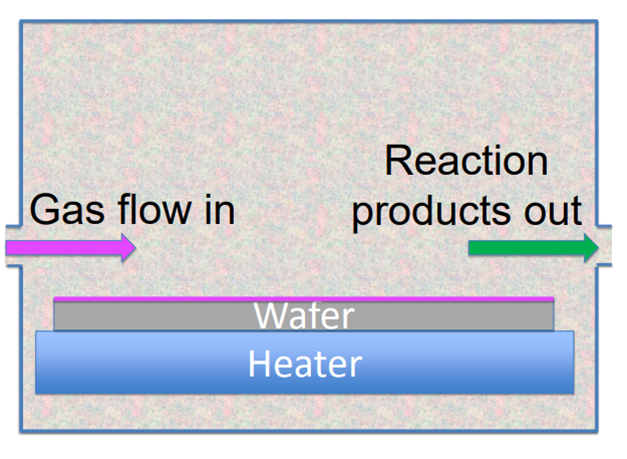
\includegraphics[width=0.5\linewidth]{CVD process.png}
    \caption{Gas flows into initially evacuated chamber, and undergoes chemical reaction at the heated wafer's surface, which leads to deposition of a thin film.}
    \label{cvd.process}
\end{figure}

A few considerations about the physics of this process:

\begin{itemize}
    \item The thermodynamics of the chemical reaction must be energetically favorable to produce a solid thin film reaction product on the wafer.
    \item Gas flows conditions must allow for uniform coating of the wafer, even though the gas is gradually depleted while flowing over it.
    \item The thickness $t$ of the produced thin film as a function of the $x$ distance from the end closer to the gas entrance port is given as follows:
    \begin{equation}
        t_{film}(x)=\exp\Big(-\frac{E_{act}}{k_BT}\Big) \times P_{growth}\times C_{gas}(x)
        \label{cvd.equation}
    \end{equation}
    where $P_{growth}$ is a probabilistic term relating to the nucleation of solid material, and $C_{gas}$ is the concentration of gas in $x$.
\end{itemize}

Equation \ref{cvd.equation} predicts that, at high temperatures, when the chemical reaction occurs more easily, the growth will enter a \textbf{mass transport-limited regime}, when the control of gas flow is the key aspect in ensuring a homogeneous coating. Intuitively, at low temperatures, growth will enter the \textbf{reaction-limited regime}.

The temperature at which this transition occurs will be largely determined by the pressure of the system, as in Figure \ref{cvd.regime}. At higher pressure, free mean path is increased, so the system will spend less time in the mass transport-limited regime, since particles can come from further away to be used in the reaction.

Because pressure plays such an important role in determining how film thickness will depend on temperature, \textbf{CVD processes are typically classified according to the pressure at which the deposition takes place.}

\begin{figure}[H]
    \centering
    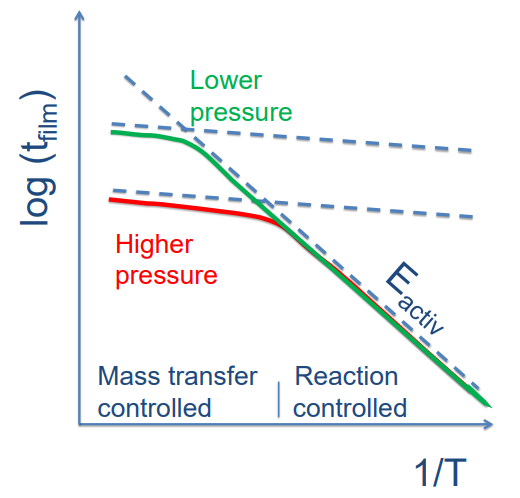
\includegraphics[width=0.5\linewidth]{cvd regimes.png}
    \caption{Pressure the determines the transition temperature between reaction-limited and mass-transport limited regimes.}
    \label{cvd.regime}
\end{figure}

\subsubsection{Classification of PVD by Pressure}

\begin{itemize}
    \item Atmospheric pressure CVD (APCVD)
    \item Sub-atmospheric pressure CVD (SACVD)
    \begin{itemize}
        \item $1000 mbar > P > 10 mbar$ ($1$ bar$\approx$ $0.987$ atm);
        \item Less interaction between gas molecules reduces chances for unwanted particle synthesis in the gas;
        \item Increased mean free path will decrease local variation of gas concentration, and increase uniformity across the wafer;
    \end{itemize}
    \item Low pressure CVD (LPCVD)
    \begin{itemize}
        \item 0.1 mbar > P > 10 mbar
    \end{itemize}
    \item Ultrahigh vacuum CVD (UHV/CVD)
    \begin{itemize}
        \item Initial vacuum $10^{-7}$ - $10^{-8}$ mbar and process occurs at $10^{-3}$ mbar
    \end{itemize}
\end{itemize}

We shall go through some of these processes in greater detail below,

\subsubsection{Classification of CVD by Reactor Type}

\begin{figure}[H]
    \centering
    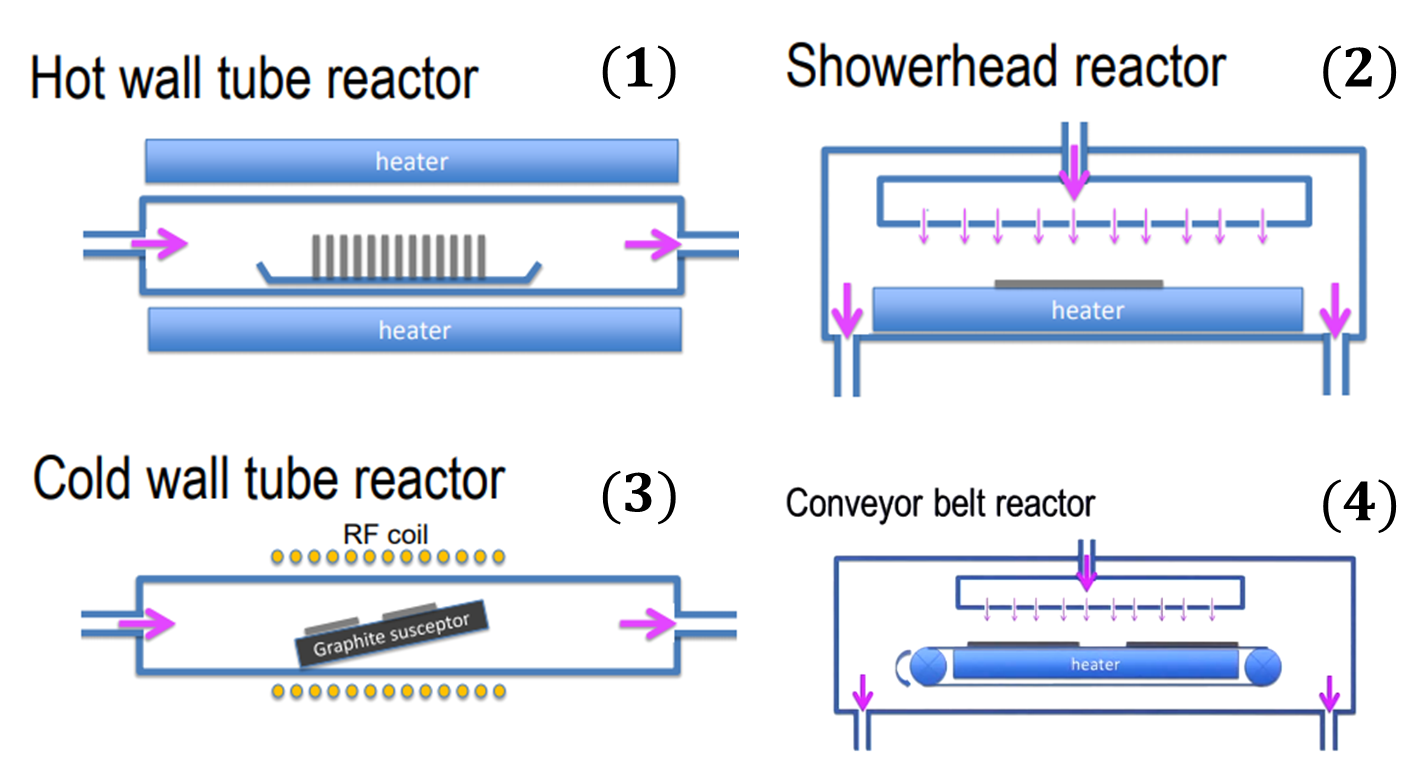
\includegraphics[width=1\linewidth]{cvd reactor type.png}
    \caption{(1) Wafers are placed in a fused silica boat and subjected to uniform temperatures. (2) Wafers are placed on a graphite susceptor and subjected to only locally high temperatures, which is tilted to avoid downstream depletion of the gas. (3)-(4) Wafer is placed on a local heater.}
    \label{fig:my_label}
\end{figure}

\subsection{Types of CVD Processes}



















\section{Physical Vapor Deposition}
\section{Litography}
\section{Dry Etching}
\section{Wet Etching}
\section{Inspection and Metrology}



\bibliographystyle{plain}
\bibliography{references.bib}




\pagebreak








\end{document}
